%%%%%%%% ICML/ICCV 2021 EXAMPLE LATEX SUBMISSION FILE %%%%%%%%%%%%%%%%%

\documentclass[10pt,twocolumn,letterpaper]{article} % comment out for ICCV style paper
%\documentclass{article} % comment out for NeurIPS style paper

\usepackage{etex}

% MN: to create different versions
%\usepackage[icml_submission]{optional}
%\usepackage[icml_accepted]{optional}
%\usepackage[for_gig]{optional}
\usepackage[iccv_submission]{optional}

\opt{iccv_submission}{
  \usepackage{iccv}
  \usepackage{times}
  \usepackage{epsfig}
  \usepackage{graphicx}
  %\usepackage[allfiguresdraft]{draftfigure}
  \usepackage{nicefrac}

  \usepackage{amsmath}
  \usepackage{amssymb}

  \definecolor{ggreen}{HTML}{115740}

  % Include other packages here, before hyperref.
  
  % If you comment hyperref and then uncomment it, you should delete
  % egpaper.aux before re-running latex.  (Or just hit 'q' on the first latex
  % run, let it finish, and you should be clear).
  \usepackage[pagebackref=true,breaklinks=true,letterpaper=true,colorlinks=true,bookmarks=false,linkcolor=ggreen,citecolor=ggreen]{hyperref}
  
  \iccvfinalcopy % *** Uncomment this line for the final submission
  
  \def\iccvPaperID{****} % *** Enter the ICCV Paper ID here
  \def\httilde{\mbox{\tt\raisebox{-.5ex}{\symbol{126}}}}

  % Pages are numbered in submission mode, and unnumbered in camera-ready
  \ificcvfinal\pagestyle{empty}\fi
}

\opt{icml_submission,for_gig}{
  \usepackage{graphicx}
  \usepackage{amsmath}
  \usepackage{amssymb}
  \usepackage[colorlinks=true,linkcolor=blue,citecolor=blue]{hyperref}
  \usepackage[table]{xcolor}
}

% Recommended, but optional, packages for figures and better typesetting:
\usepackage{microtype}
\usepackage{subfigure}
\usepackage{booktabs} % for professional tables
\usepackage{enumitem}
\usepackage{amsfonts}
\usepackage{tikz}

\usetikzlibrary{arrows.meta, % if the figure contains arrow-tips
                bending,     % arrow tips on arcs are "bent," i.e., deformed a bit
                patterns     % if the figure contains pattern fills
               }

\usetikzlibrary{spy}
\usetikzlibrary{arrows,shapes,automata,backgrounds,petri,positioning}
\usetikzlibrary{decorations.pathmorphing}
\usetikzlibrary{decorations.shapes}
\usetikzlibrary{decorations.text}
\usetikzlibrary{decorations.fractals}
\usetikzlibrary{decorations.footprints}
\usetikzlibrary{shadows}

\renewcommand\floatpagefraction{.99}
\renewcommand\topfraction{.99}
\renewcommand\bottomfraction{.99}
\renewcommand\textfraction{.01}   
\setcounter{totalnumber}{50}
\setcounter{topnumber}{50}
\setcounter{bottomnumber}{50}

%\setlength{\textfloatsep}{0.25\baselineskip plus 0.2\baselineskip minus 0.5\baselineskip}
%\setlength{\textfloatsep}{1.25\baselineskip plus 0.2\baselineskip minus 0.5\baselineskip}

\DeclareMathOperator{\id}{Id}
\newcommand{\fxpsi}{\Phi_{\theta}^{BA}}
\newcommand{\fxvarphi}{\Phi_{\theta}^{AB}}
\newcommand{\fxpsivarepsilon}{\Phi_{\theta \varepsilon}^{BA}}
\newcommand{\fxvarphivarepsilon}{\Phi_{\theta \varepsilon}^{AB}}
\graphicspath{{figs/}}

\newcommand{\mn}[1]{{\color{black}{#1}}}
\newcommand{\mnl}[1]{{\color{red}{$\leftarrow$~#1}}}
\newcommand{\mnr}[1]{{\color{red}{#1~$\rightarrow$}}}
\newcommand{\zp}[1]{{\color{blue}{#1}}}

% hyperref makes hyperlinks in the resulting PDF.
% If your build breaks (sometimes temporarily if a hyperlink spans a page)
% please comment out the following usepackage line and replace
% \usepackage{icml2021} with \usepackage[nohyperref]{icml2021} above.
%\usepackage{hyperref}

% Attempt to make hyperref and algorithmic work together better:
\newcommand{\theHalgorithm}{\arabic{algorithm}}

\opt{icml_submission}{
% Use the following line for the initial blind version submitted for review:
\usepackage{icml2021}

\usepackage{setspace}
\usepackage[labelfont={bf,small},font={small,stretch=1.1}]{caption}
%\usepackage{subcaption}

\usepackage[colorinlistoftodos,prependcaption,textsize=tiny]{todonotes}
}

\opt{icml_accepted}{
% If accepted, instead use the following line for the camera-ready submission:
  \usepackage[accepted]{icml2021}
}

\opt{for_gig}{
  \usepackage[accepted]{icml2021_unpublished_draft}
  \usepackage[colorinlistoftodos,prependcaption,textsize=tiny,disable]{todonotes}
  % disable todos
  %\usepackage[colorinlistoftodos,prependcaption,textsize=tiny,disable]{todonotes}
}

\usepackage[labelfont={bf,small},font={small}]{caption}
\begin{document}

\sloppy

\opt{iccv_submission}{
  %%%%%%%%% TITLE
\title{ICON: Learning Regular Maps Through Inverse Consistency}

\author{Hastings Greer\\
  Department of Computer Science\\
UNC Chapel Hill, USA\\
{\tt\small tgreer@cs.unc.edu}
% For a paper whose authors are all at the same institution,
% omit the following lines up until the closing ``}''.
% Additional authors and addresses can be added with ``\and'',
% just like the second author.
% To save space, use either the email address or home page, not both
\and
Roland Kwitt\\
Department of Computer Science\\
University of Salzburg, Austria\\
{\tt\small Roland.Kwitt@sbg.ac.at}
\and
Fran\c{c}ois-Xavier Vialard\\
LIGM, Universit\'e Gustave Eiffel, France\\
{\tt\small francois-xavier.vialard@u-pem.fr}
\and
Marc Niethammer\\
 Department of Computer Science\\
UNC Chapel Hill, USA\\
{\tt\small mn@cs.unc.edu}
}

\maketitle

\thispagestyle{plain}
\pagestyle{plain}

% Remove page # from the first page of camera-ready.
\ificcvfinal\thispagestyle{empty}\fi
}

\opt{for_gig,icml_submission}{

% The \icmltitle you define below is probably too long as a header.
% Therefore, a short form for the running title is supplied here:
%\icmltitlerunning{Inverse Consistency is Almost All You Need}
\icmltitlerunning{Learning Regular Maps Through Inverse Consistency}
  
\twocolumn[
%\icmltitle{Inverse Consistency is All You Need \\ -- for Image Registration}
\icmltitle{Learning Regular Maps Through Inverse Consistency}

% It is OKAY to include author information, even for blind
% submissions: the style file will automatically remove it for you
% unless you've provided the [accepted] option to the icml2021
% package.

% List of affiliations: The first argument should be a (short)
% identifier you will use later to specify author affiliations
% Academic affiliations should list Department, University, City, Region, Country
% Industry affiliations should list Company, City, Region, Country

% You can specify symbols, otherwise they are numbered in order.
% Ideally, you should not use this facility. Affiliations will be numbered
% in order of appearance and this is the preferred way.
\icmlsetsymbol{equal}{*}

\begin{icmlauthorlist}
\icmlauthor{Hastings Greer}{unc}
\icmlauthor{Roland Kwitt}{salzburg}
\icmlauthor{Fran\c{c}ois Xavier-Vialard}{upem}
\icmlauthor{Marc Niethammer}{unc}
\end{icmlauthorlist}

\icmlaffiliation{unc}{Department of Computer Science, University of North Carolina at Chapel Hill, USA}
\icmlaffiliation{salzburg}{Department of Computer Science, University of Salzburg, Austria}
\icmlaffiliation{upem}{LIGM, Universit\'e Gustave Eiffel, France}

\icmlcorrespondingauthor{Hastings Greer}{tgreer@cs.unc.edu}

% You may provide any keywords that you
% find helpful for describing your paper; these are used to populate
% the "keywords" metadata in the PDF but will not be shown in the document
\icmlkeywords{Deep Learning, Image Registration, Inverse Consistency}

\vskip 0.3in
]

% this must go after the closing bracket ] following \twocolumn[ ...

% This command actually creates the footnote in the first column
% listing the affiliations and the copyright notice.
% The command takes one argument, which is text to display at the start of the footnote.
% The \icmlEqualContribution command is standard text for equal contribution.
% Remove it (just {}) if you do not need this facility.

%\printAffiliationsAndNotice{}  % leave blank if no need to mention equal contribution
\printAffiliationsAndNotice{\icmlEqualContribution} % otherwise use the standard text.
}


\begin{abstract}
  Learning maps between data samples is fundamental. Applications range from representation learning, image translation and generative modeling, to the estimation of spatial deformations. Such maps relate feature vectors, or map between feature spaces. Well-behaved maps should be regular, which can be imposed explicitly or may emanate from the data itself. We explore what induces regularity for spatial transformations, e.g., when computing image registrations. Classical optimization-based models compute maps between pairs of samples and rely on an appropriate regularizer for well-posedness. Recent deep learning approaches have attempted to avoid using such regularizers altogether by relying on the sample population instead. We explore if it is possible to obtain spatial regularity using an inverse consistency loss only and elucidate what explains map regularity in such a context. We find that deep networks combined with an inverse consistency loss and randomized off-grid interpolation yield well behaved, approximately diffeomorphic, spatial transformations. Despite the simplicity of this approach, our experiments present compelling evidence, on both synthetic and real data, that regular maps can be obtained without carefully tuned explicit regularizers, \mn{while achieving competitive registration performance.}%and only marginal degradation in registration performance.
  %for binary shapes and textured images. 
  % Aside from obtaining competitive performance on synthetic and real data, our approach opens up the possibility for simple application-specific models and 
  % simplifies regularizer tuning.


%  Image registration, in particular nonparametric approaches, relies on regularizing transformations to make the underlying optimization problems well-posed. Thereby addressing the famous aperture effect. How to pick an appropriate regularizer is non-trivial, depends on the particular application, makes finding a good model difficult, and has therefore been explored widely. Furthermore, much effort has been invested in designing registration algorithms which can assure diffeomorphic transformations. We challenge the need for these explicit, complicated modeling assumptions. Instead, we show how to achieve diffeomorphic transformations \emph{from data}, simply by encouraging inverse consistency over a large training set \emph{without} further regularization. In the context of traditional pair-wise registration formulations such an approach would be an improper, heretic Al idea. However, it makes sense for neural network based registration models trained on large datasets. Importantly, this approach opens up the possibility for much simpler application-specific registration algorithms, and effectively eliminates regularizer tuning.
  
%Image registration, in particular nonparametric approaches, relies on regularizing transformations to make the underlying optimization problems well-posed. Thereby addressing the famous aperture effect. How to pick an appropriate regularizer is non-trivial, depends on the particular application, makes finding a good model difficult, and has therefore been explored widely. Furthermore, much effort has been invested in designing registration algorithms which can assure diffeomorphic transformations. We challenge the need for these explicit, complicated modeling assumptions. Instead, we show how to achieve diffeomorphic transformations \emph{from data}, simply by encouraging inverse consistency over a large training set \emph{without} further regularization. In the context of traditional pair-wise registration formulations such an approach would be an improper, heretic Al idea. However, it makes sense for neural network based registration models trained on large datasets. Importantly, this approach opens up the possibility for much simpler application-specific registration algorithms, and effectively eliminates regularizer tuning.
\end{abstract}

\section{Motivation}
\label{section:motivation}

Learning maps between feature vectors or spaces is an important task. Feature vector maps are used to improve representation learning~\cite{chen2020exploring}, or to learn correspondences in natural language processing~\cite{blitzer2006domain}. Maps between spaces are important for generative models when using normalizing flows~\cite{kobyzev2020normalizing} (to map between a simple and a complex probability distribution), or to determine spatial correspondences between images, \eg, for optical flow~\cite{horn1981determining} to determine motion from videos~\cite{fortun2015optical}, depth estimation from stereo images~\cite{laga2020survey}, or medical image registration~\cite{sotiras2013deformable,tustison2019learning}.

\vskip0.5ex
Regular maps are typically desired; \eg, diffeomorphic maps for normalizing flows to properly map densities, or for medical image registration to map to an atlas space~\cite{joshi2004unbiased}. Estimating such maps requires an appropriate choice of transformation model. This entails picking a parameterization, which can be simple and depend on few parameters (\eg, an affine transformation), or which can have millions of parameters for 3D nonparametric approaches~\cite{holden2007review}. Regularity is achieved by 1) picking a simple transformation model with limited degrees of freedom, 2) regularization of the transformation parameters, 3) or implicitly through the data itself. Our goal is to demonstrate and understand how spatial regularity of a transformation can be achieved by encouraging \emph{inverse consistency} of a map. Our motivating example is image registration/optical flow, but our results are applicable to other tasks where spatial transformations are sought. %, such as the ones discussed in the preceding paragraph.

%Image registration is the process of estimating spatial correspondences between images. It is an essential task for many medical applications, e.g., to register to a common atlas space for analysis, to assess changes over time, or to reconcile planning and treatment images in the presence of spatial deformations.

\vskip0.5ex
Registration problems have traditionally been solved by numerical optimization~\cite{modersitzki2004numerical} of a loss function balancing an image similarity measure and a regularizer. Here, the predominant paradigm is \emph{pair-wise} image registration\footnote{A notable exception is congealing~\cite{zollei2005efficient}.} where many maps may yield good image similarities between a transformed moving and a fixed image; the regularizer is required for well-posedness to single out the most desirable map. Many different regularizers have been proposed~\cite{holden2007review,modersitzki2004numerical,risser2011simultaneous} and many have multiple hyperparameters, making regularizer choice and tuning difficult in practice. Deep learning approaches to image registration and optical flow have moved to learning maps from \emph{many image pairs}, which raises the question if explicit spatial regularization is still required, or if it will emanate as a consequence of learning over many image pairs. For optical flow, encouraging results have been obtained without using a spatial regularizer~\cite{dosovitskiy2015flownet,ranjan2017optical}, though more recent work has advocated for spatial regularization to avoid ``vague flow boundaries and undesired artifacts''~\cite{hui2018liteflownet,hur2019iterative}. Interestingly, for medical image registration, where map regularity is often very important, almost all the existing work uses regularizers as initially proposed for pairwise image registration~\cite{shen19,yang2017quicksilver,balakrishnan2019voxelmorph} with the notable exception of~\cite{bhalodia19} where the deformation space is guided by an autoencoder instead.

\vskip0.5ex
Limited work explores if regularization for deep registration networks can be avoided entirely, or if weaker forms of regularizations might be sufficient. To help investigate this question, we work with binary shapes (where regularization is particularly important due to the aperture effect~\cite{horn1986robot}) and real images. We show that regularization is necessary, but that carefully encouraging \emph{inverse consistency} of a map suffices to obtain approximate diffeomorphisms. The result is a simple, yet effective, nonparametric approach to obtain well-behaved maps, which only requires limited tuning. In particular, the in practice often highly challenging process of selecting a spatial regularizer is eliminated.

%\todo[inline]{mn: we should find a good terminoloy to talk about this. we still use a form of regularization, but it is much weaker than the standard regularization, because it doesn't depend on penalizing spatial derivatives in any form. Not sure how to best keep these two types of regularization apart wrt. terminology. Suggestions are welcome. Maybe call one spatial regularization and the other one inverse consistency regularization?}
%\todo[inline]{Hastings: I like inverse consistency regularization}
%\todo[inline]{rk: I propose ``weak regularization'', similar to the term ``weakly-labeled data'' that is commonly used when ``strong'' (detailed) labels are not available?} 

\vskip0.5ex
\noindent {\bf Our contributions} are as follows: (1) We show that \emph{approximate} inverse consistency, combined with off-grid interpolation, results in approximate diffeomorphisms, when using a deep registration model trained on large datasets. Foregoing regularization is insufficient; (2) Bottleneck layers are not required and many network architectures are suitable; (3) Affine preregistration is \mn{not required}; (4) We propose randomly sampled evaluations to avoid transformation flips in texture-less areas and an inverse consistency loss with beneficial boundary effects; (5) We present good results of our approach on synthetic data, MNIST, and a 3D magnetic resonance knee dataset \mn{of the Osteoarthritis Initiative (OAI).}

% \noindent {\bf Our contributions} are summarized below:
% \begin{itemize}[noitemsep,topsep=0pt,parsep=0pt,partopsep=0pt, leftmargin=13pt]
% \item[1)] We show that \emph{approximate} inverse consistency, combined with off-grid interpolation, results in approximate diffeomorphisms, when using a deep registration model trained on large datasets. Foregoing regularization is insufficient.
% \item[2)] We show that bottleneck layers are not required and many network architectures are suitable.
% \item[3)] We show that affine preregistration is optional. % Our approach can capture affine transformation components, but also benefits from affine preregistration.
% \item[4)] We propose randomly sampled evaluations to avoid transformation flips in texture-less areas and an inverse consistency loss with beneficial boundary effects.
% \item[5)] We show good results of our approach on synthetic data, MNIST, and a 3D magnetic resonance knee dataset. %, showing state-of-the-art performance.
% \end{itemize}

%\todo[inline]{We should find a catchy acronym for branding. How about Deep RegUlarity InDuced (DRUID) registration. Open, of course, to other options. Though this could let us say: DRUID works like magic :) }

\section{Background and Analysis}
\label{section:background}

Image registration is typically based on solving  optimization problems of the form
\begin{equation}
  \theta^* = \underset{\theta}{\text{argmin}}~\mathcal{L}_{\text{sim}}(I^A\circ \Phi^{-1}_\theta,I^B) + \lambda\mathcal{L}_{\text{reg}}(\theta)\enspace,\label{eq:basic_reg}
\end{equation}
where $I^A$ and $I^B$ are moving and fixed images, $\mathcal{L}_{\text{sim}}(\cdot,\cdot)$ is the similarity measure, $\mathcal{L}_{\text{reg}}(\cdot)$ is a regularizer%\footnote{A regularizer typically encourages amooth transformations.}
, $\theta$ are the transformation parameters, $\Phi_\theta$ is the transformation map, and $\lambda\geq 0$. We consider images as functions from $\mathbb{R}^N$ to $\mathbb{R}$ and maps as functions from $\mathbb{R}^N$ to $\mathbb{R}^N$. We write $\|f\|_p$ for the $L^p$ norm on a scalar or vector-valued function $f$.

\vskip0.5ex
Maps, $\Phi_\theta$, can be parameterized using few parameters (\eg, affine, B-spline~\cite{holden2007review}) or nonparametrically with continuous vector fields~\cite{modersitzki2004numerical}. In the nonparametric case, parameterizations are infinite-dimensional (as one deals with function spaces) and represent displacement, velocity, or momentum fields~\cite{balakrishnan2019voxelmorph,shen19,yang2017quicksilver,modersitzki2004numerical}. Solutions to Eq.~\eqref{eq:basic_reg} are classically obtained via numerical optimization~\cite{modersitzki2004numerical}. Recent deep registration networks are conceptually similar, but \emph{predict} $\tilde{\theta}^*$, \ie, an estimate of the true minimizer $\theta^*$. %, and by using  many samples for training instead of \emph{optimizing} over a single $(I_0,I_1)$ pair.

\vskip0.5ex
There are three interesting observations: \emph{First}, for transformation models with few parameters (\eg, affine), regularization is often not used (\ie, $\lambda=0$). \emph{Second}, while deep learning (DL) models minimize losses similar to Eq.~\eqref{eq:basic_reg}, the parameterization is different: it is over network \emph{weights}, resulting in a predicted $\theta^*$ instead of optimizing over $\theta$ directly. \emph{Third}, DL models are trained over \emph{large collections of image pairs} instead of a single $(I^A,I^B)$ pair. This raises the following questions: \textbf{Q1}) Is explicit spatial regularization necessary, or can we avoid it for nonparametric registration models? \textbf{Q2}) Is using a \emph{single} neural network parameterization to predict \emph{all} $\theta^*$ beneficial? For instance, will it result in simple solutions as witnessed for deep networks on other tasks~\cite{shah2020pitfalls} or capture meaningful deformation spaces as observed in~\cite{yang2017quicksilver}? \textbf{Q3}) %\todo{We technically do not show this. Can we add one of these results to one of the figures?}
Does a deep network parameterization itself result in regular solutions, even if only applied to a single image pair, as such effects have, \eg, been observed for structural optimization~\cite{hoyer2019neural}?

\vskip0.5ex
Regularization typically encourages spatial smoothness by penalizing derivatives (or smoothing in dual space). Commonly, one uses a Sobolev norm or total variation. Ideally, one would like a regularizer adapted to deformations one expects to see (as it encodes a prior on expected deformations \eg, as in~\cite{niethammer2019metric}). In consequence, picking and tuning a regularizer is cumbersome and often involves many hyperparameters. While avoiding explicit regularization has been explored for deep registration / optical flow networks~\cite{dosovitskiy2015flownet,ranjan2017optical},  there is evidence that regularization is beneficial~\cite{hui2018liteflownet}. 

\vskip0.5ex
\emph{Our key idea is to avoid complex spatial regularization and to instead obtain approximate diffeomorphisms by encouraging inverse consistent maps \mn{via regularization}.}


%replacing it by an inverse consistency loss, i.e., an inverse consistency regularizer, when combined with a deep network parameterization, with training over large numbers of image pairs, and with randomized (i.e., off-grid) evaluations of the consistency loss.
%Intuitively, if one can achieve inverse consistency while at least assuring continuous maps, one obtains diffeomorphic transformations \emph{without explicitly enforcing spatial smoothness} as a diffeomorphism is nothing else than a smooth (here continuous) map with a smooth inverse.
%\todo[inline]{Might need to be careful with the diffeo statement here. What can we really say about the transformations that are being outputted here.}


%\subsection{Weakly-Regularized Nonparametric Registration}
\subsection{Weakly-regularized registration}
\label{subsection:regularization_thoughts_and_sorting}

Assume we eliminate regularization ($\lambda=0$) and use the $p$-th power of the $L^p$ norm of the difference between the warped image, $I^A\circ\Phi_\theta^{-1}$, and the fixed image, $I^B$, as similarity measure. Then, our optimization problem becomes
\begin{equation}
  \theta^* = \underset{\theta}{\arg \min}~\int (I^A(\Phi_\theta^{-1}(x))-I^B(x))^p~\mathrm{d}x\,,~p\geq 1, \label{eq:only_similarity}
\end{equation}
\ie, the image intensities of $I^A$ should be close to the image intensities of $I^B$ \emph{after} deformation. Without regularization, we are entirely free to choose $\Phi_\theta$. Highly irregular minimizers of Eq.~\eqref{eq:only_similarity} may result as each intensity value $I^A$ is simply matched to the closest intensity value of $I^B$ regardless of location. For instance, for a constant $I^B(x)=c$ and a moving image $I^A(y)$ with a unique location $y_c$, where $I^A(y_c)=c$, the optimal map is $\Phi_\theta^{-1}(x) = y_c$, which  is not invertible: only \emph{one point} of $I^A$ will be mapped to the \emph{entire} domain of $I^B$. Clearly, more spatial regularity is desirable. Importantly, irregular deformations are common optimizers of Eq.~\eqref{eq:only_similarity}. 

\vskip1ex
Optimal mass transport (OMT) is widely used in machine learning and in imaging. Such models are of interest to us as they can be inverse consistent. An OMT variant of the discrete reformulation of Eq.~\eqref{eq:only_similarity} is
\begin{equation}
    \theta^* = \underset{\theta}{\arg\min}~\mathrm{d}x \sum_{i=1}^S (I^A(\Phi_\theta^{-1}(x_i))-I^B(x_i))^p\,, p\geq 1\label{eq:only_similarity_discrete}
\end{equation}
%\todo[inline]{FX: are these explanations below correct? Maybe we should write this a bit more formally. I was just shooting for some high level intuition so far}
for $p\geq 1$, where $i$ indexes the $S$ grid points $x_i$, $\Phi_\theta^{-1}(x_i)$ is restricted to map to the grid \mn{points} $y_i$ of $I^A$, and $\mathrm{d}x$ is the discrete area element. Instead of considering all possible maps, we attach a unit mass to each \emph{intensity} value of $I^A$ and $I^B$ and ask for minimizers of Eq.~\eqref{eq:only_similarity_discrete} which transform the intensity distribution of $I^A$ to the intensity distribution of $I^B$ via \emph{permutations} of the values only. As we only allow permutations, the optimal map will be \emph{invertible} by construction. This problem is equivalent to optimal mass transport for one-dimensional empirical measures~\cite{peyre2019computational}. One obtains the optimal value by ordering all intensity values of $I^A$ ($I^A_1\leq \cdots\leq I^A_S$) and $I^B$ ($I^B_1\leq \cdots\leq I^B_S$). The minimum is the $p$-th power of the  $p$-Wasserstein distance ($p\geq 1$) 
$\mathcal{W}_p^p = \sum_i |I^A_i-I^B_i|^p$.
%(or in general by the p-th power of the p-Wasserstein distance ($p\geq 1$) when penalizing $|x-y|^p$ instead of $|x-y|^2$) can then simply be computed as 
%is then simply
%\begin{equation}
%    \mathcal{W}_p^p = \sum_{i=1}^S |I^A_i-I^B_i|^p\,.
%\end{equation}
In consequence, minimizers for Eq.~\eqref{eq:only_similarity} are related to sorting, but do not consider spatial regularity. Note that solutions might not be unique when intensity values in $I^A$ or $I^B$ are repeated. 
%Solutions will be invertible when using the Monge form of optimal transport, but might not be in the Kantorovich formulation where mass is allowed to split~\cite{peyre2019computational}.
Solutions via sorting were empirically explored for registration in~\cite{Rholfing12} to illustrate that they, in general, do not result in spatially meaningful registrations.
%Based on these considerations
At this point, our idea of using inverse consistency (\ie, invertible maps)
as the only regularizer appears questionable, given that OMT often provides an inverse consistent model (when a matching, \ie, a Monge solution, is optimal), while resulting in irregular maps (Fig.~\ref{fig:matching_examples}).

\vskip0.5ex
\emph{\mn{Yet, we will show that a registration network, combined with %a careful implementation of
  an inverse consistency loss, encourages map regularity.}}
%continuous maps (and even more regular diffeomorphisms).}

%it is highly related to the Monge problem discussed above, which 


\begin{figure}
  \centering
  \includegraphics[width=0.98\columnwidth]{src_tgt.pdf}
%   \begin{tabular}{cc}
% %    (b) Two SSD mapping solutions &
% %    (c) Two OMT mapping solutions \\
%     {\footnotesize (a) Source function} & {\footnotesize (b) Target function} \\
%     \resizebox{0.43\columnwidth}{!}
%     {
%       \input{./xfig_figs/mse_omt_functions_illustration_I0.tikz}
%     }
%     &
%     \resizebox{0.43\columnwidth}{!}
%     {
%       {\pgfkeys{/pgf/fpu/.try=false}%
\ifx\XFigwidth\undefined\dimen1=0pt\else\dimen1\XFigwidth\fi
\divide\dimen1 by 3195
\ifx\XFigheight\undefined\dimen3=0pt\else\dimen3\XFigheight\fi
\divide\dimen3 by 1578
\ifdim\dimen1=0pt\ifdim\dimen3=0pt\dimen1=3946sp\dimen3\dimen1
  \else\dimen1\dimen3\fi\else\ifdim\dimen3=0pt\dimen3\dimen1\fi\fi
\tikzpicture[x=+\dimen1, y=+\dimen3]
{\ifx\XFigu\undefined\catcode`\@11
\def\temp{\alloc@1\dimen\dimendef\insc@unt}\temp\XFigu\catcode`\@12\fi}
\XFigu3946sp
% Uncomment to scale line thicknesses with the same
% factor as width of the drawing.
%\pgfextractx\XFigu{\pgfqpointxy{1}{1}}
\ifdim\XFigu<0pt\XFigu-\XFigu\fi
\pgfdeclarearrow{
  name = xfiga2,
  parameters = {
    \the\pgfarrowlinewidth \the\pgfarrowlength \the\pgfarrowwidth\ifpgfarrowopen o\fi},
  defaults = {
	  line width=+7.5\XFigu, length=+120\XFigu, width=+60\XFigu},
  setup code = {
    % miter protrusion = thk * sqrt(wd^2 + (tipmv*len)^2) / (2 * wd)
    \dimen7 2.6\pgfarrowlength\pgfmathveclen{\the\dimen7}{\the\pgfarrowwidth}
    \dimen7 2\pgfarrowwidth\pgfmathdivide{\pgfmathresult}{\the\dimen7}
    \dimen7 \pgfmathresult\pgfarrowlinewidth
    \pgfarrowssettipend{+\dimen7}
    \pgfarrowssetbackend{+-1.25\pgfarrowlength}
    \dimen9 -\pgfarrowlength\advance\dimen9 by-0.5\pgfarrowlinewidth
    \pgfarrowssetlineend{+\dimen9}
    \dimen9 -\pgfarrowlength\advance\dimen9 by-0.5\pgfarrowlinewidth
    \pgfarrowssetvisualbackend{+\dimen9}
    \pgfarrowshullpoint{+\dimen7}{+0pt}
    \pgfarrowsupperhullpoint{+-1.25\pgfarrowlength}{+0.5\pgfarrowwidth}
    \pgfarrowssavethe\pgfarrowlinewidth
    \pgfarrowssavethe\pgfarrowlength
    \pgfarrowssavethe\pgfarrowwidth
  },
  drawing code = {\pgfsetdash{}{+0pt}
    \ifdim\pgfarrowlinewidth=\pgflinewidth\else\pgfsetlinewidth{+\pgfarrowlinewidth}\fi
    \pgfpathmoveto{\pgfqpoint{-1.25\pgfarrowlength}{-0.5\pgfarrowwidth}}
    \pgfpathlineto{\pgfqpoint{0pt}{0pt}}
    \pgfpathlineto{\pgfqpoint{-1.25\pgfarrowlength}{0.5\pgfarrowwidth}}
    \pgfpathlineto{\pgfqpoint{-\pgfarrowlength}{0pt}}
    \pgfpathclose
    \ifpgfarrowopen\pgfusepathqstroke\else\pgfsetfillcolor{.}
	\ifdim\pgfarrowlinewidth>0pt\pgfusepathqfillstroke\else\pgfusepathqfill\fi\fi
  }
}
\clip(117,-4494) rectangle (3312,-2916);
\tikzset{inner sep=+0pt, outer sep=+0pt}
\pgfsetfillcolor{black}
\pgftext[base,at=\pgfqpointxy{300}{-3750},rotate=+90] {\fontsize{12}{14.4}\normalfont $I^B(x)$}
\pgfsetlinewidth{+7.5\XFigu}
\pgfsetcolor{black}
\filldraw  (1050,-3600) circle [radius=+75];
\filldraw  (2250,-3450) circle [radius=+75];
\filldraw  (1650,-3450) circle [radius=+75];
\filldraw  (2850,-4200) circle [radius=+75];
\draw (750,-4275)--(750,-4125);
\draw (1050,-4275)--(1050,-4125);
\draw (1350,-4275)--(1350,-4125);
\draw (1650,-4275)--(1650,-4125);
\draw (1950,-4275)--(1950,-4125);
\draw (2250,-4275)--(2250,-4125);
\pgfsetarrows{[line width=7.5\XFigu]}
\pgfsetarrowsend{xfiga2}
\draw (300,-4200)--(3300,-4200);
\draw (450,-4350)--(450,-3150);
\pgfsetarrowsend{}
\draw (2550,-4275)--(2550,-4125);
\draw (2850,-4275)--(2850,-4125);
\draw (525,-3900)--(375,-3900);
\draw (525,-3600)--(375,-3600);
\draw (450,-4200)--(1050,-3600);
\draw (1050,-3600)--(1650,-3450);
\draw (1650,-3450)--(2250,-3450);
\draw (2250,-3450)--(2850,-4200);
\pgftext[base,left,at=\pgfqpointxy{900}{-3075}] {\fontsize{12}{14.4}\normalfont $1.0$}
\pgftext[base,left,at=\pgfqpointxy{1500}{-3075}] {\fontsize{12}{14.4}\normalfont $1.25$}
\pgftext[base,left,at=\pgfqpointxy{2100}{-3075}] {\fontsize{12}{14.4}\normalfont $1.25$}
\pgftext[base,left,at=\pgfqpointxy{2700}{-3075}] {\fontsize{12}{14.4}\normalfont $0.0$}
\pgftext[base,left,at=\pgfqpointxy{300}{-3075}] {\fontsize{12}{14.4}\normalfont $0.0$}
\pgftext[base,at=\pgfqpointxy{3225}{-4425}] {\fontsize{12}{14.4}\normalfont $x$}
\filldraw  (450,-4200) circle [radius=+75];
\endtikzpicture}%

%     }
%     \\
%     {\footnotesize (c) MSE map example} & {\footnotesize (d) OMT map example} \\
%     \resizebox{0.43\columnwidth}{!}
%     {
%       {\pgfkeys{/pgf/fpu/.try=false}%
\ifx\XFigwidth\undefined\dimen1=0pt\else\dimen1\XFigwidth\fi
\divide\dimen1 by 3174
\ifx\XFigheight\undefined\dimen3=0pt\else\dimen3\XFigheight\fi
\divide\dimen3 by 1578
\ifdim\dimen1=0pt\ifdim\dimen3=0pt\dimen1=3946sp\dimen3\dimen1
  \else\dimen1\dimen3\fi\else\ifdim\dimen3=0pt\dimen3\dimen1\fi\fi
\tikzpicture[x=+\dimen1, y=+\dimen3]
{\ifx\XFigu\undefined\catcode`\@11
\def\temp{\alloc@1\dimen\dimendef\insc@unt}\temp\XFigu\catcode`\@12\fi}
\XFigu3946sp
% Uncomment to scale line thicknesses with the same
% factor as width of the drawing.
%\pgfextractx\XFigu{\pgfqpointxy{1}{1}}
\ifdim\XFigu<0pt\XFigu-\XFigu\fi
\pgfdeclarearrow{
  name = xfiga1,
  parameters = {
    \the\pgfarrowlinewidth \the\pgfarrowlength \the\pgfarrowwidth\ifpgfarrowopen o\fi},
  defaults = {
	  line width=+7.5\XFigu, length=+120\XFigu, width=+60\XFigu},
  setup code = {
    % miter protrusion = thk * sqrt(wd^2 + (tipmv*len)^2) / (2 * wd)
    \dimen7 2.1\pgfarrowlength\pgfmathveclen{\the\dimen7}{\the\pgfarrowwidth}
    \dimen7 2\pgfarrowwidth\pgfmathdivide{\pgfmathresult}{\the\dimen7}
    \dimen7 \pgfmathresult\pgfarrowlinewidth
    \pgfarrowssettipend{+\dimen7}
    \pgfarrowssetbackend{+-\pgfarrowlength}
    \dimen9 -\pgfarrowlength\advance\dimen9 by-0.45\pgfarrowlinewidth
    \pgfarrowssetlineend{+\dimen9}
    \dimen9 -\pgfarrowlength\advance\dimen9 by-0.5\pgfarrowlinewidth
    \pgfarrowssetvisualbackend{+\dimen9}
    \pgfarrowshullpoint{+\dimen7}{+0pt}
    \pgfarrowsupperhullpoint{+-\pgfarrowlength}{+0.5\pgfarrowwidth}
    \pgfarrowssavethe\pgfarrowlinewidth
    \pgfarrowssavethe\pgfarrowlength
    \pgfarrowssavethe\pgfarrowwidth
  },
  drawing code = {\pgfsetdash{}{+0pt}
    \ifdim\pgfarrowlinewidth=\pgflinewidth\else\pgfsetlinewidth{+\pgfarrowlinewidth}\fi
    \pgfpathmoveto{\pgfqpoint{-\pgfarrowlength}{-0.5\pgfarrowwidth}}
    \pgfpathlineto{\pgfqpoint{0pt}{0pt}}
    \pgfpathlineto{\pgfqpoint{-\pgfarrowlength}{0.5\pgfarrowwidth}}
    \pgfpathclose
    \ifpgfarrowopen\pgfusepathqstroke\else\pgfsetfillcolor{.}
	\ifdim\pgfarrowlinewidth>0pt\pgfusepathqfillstroke\else\pgfusepathqfill\fi\fi
  }
}
\pgfdeclarearrow{
  name = xfiga2,
  parameters = {
    \the\pgfarrowlinewidth \the\pgfarrowlength \the\pgfarrowwidth\ifpgfarrowopen o\fi},
  defaults = {
	  line width=+7.5\XFigu, length=+120\XFigu, width=+60\XFigu},
  setup code = {
    % miter protrusion = thk * sqrt(wd^2 + (tipmv*len)^2) / (2 * wd)
    \dimen7 2.6\pgfarrowlength\pgfmathveclen{\the\dimen7}{\the\pgfarrowwidth}
    \dimen7 2\pgfarrowwidth\pgfmathdivide{\pgfmathresult}{\the\dimen7}
    \dimen7 \pgfmathresult\pgfarrowlinewidth
    \pgfarrowssettipend{+\dimen7}
    \pgfarrowssetbackend{+-1.25\pgfarrowlength}
    \dimen9 -\pgfarrowlength\advance\dimen9 by-0.5\pgfarrowlinewidth
    \pgfarrowssetlineend{+\dimen9}
    \dimen9 -\pgfarrowlength\advance\dimen9 by-0.5\pgfarrowlinewidth
    \pgfarrowssetvisualbackend{+\dimen9}
    \pgfarrowshullpoint{+\dimen7}{+0pt}
    \pgfarrowsupperhullpoint{+-1.25\pgfarrowlength}{+0.5\pgfarrowwidth}
    \pgfarrowssavethe\pgfarrowlinewidth
    \pgfarrowssavethe\pgfarrowlength
    \pgfarrowssavethe\pgfarrowwidth
  },
  drawing code = {\pgfsetdash{}{+0pt}
    \ifdim\pgfarrowlinewidth=\pgflinewidth\else\pgfsetlinewidth{+\pgfarrowlinewidth}\fi
    \pgfpathmoveto{\pgfqpoint{-1.25\pgfarrowlength}{-0.5\pgfarrowwidth}}
    \pgfpathlineto{\pgfqpoint{0pt}{0pt}}
    \pgfpathlineto{\pgfqpoint{-1.25\pgfarrowlength}{0.5\pgfarrowwidth}}
    \pgfpathlineto{\pgfqpoint{-\pgfarrowlength}{0pt}}
    \pgfpathclose
    \ifpgfarrowopen\pgfusepathqstroke\else\pgfsetfillcolor{.}
	\ifdim\pgfarrowlinewidth>0pt\pgfusepathqfillstroke\else\pgfusepathqfill\fi\fi
  }
}
\clip(3738,-2694) rectangle (6912,-1116);
\tikzset{inner sep=+0pt, outer sep=+0pt}
\pgfsetlinewidth{+7.5\XFigu}
\pgfsetstrokecolor{blue}
\pgfsetarrows{[line width=7.5\XFigu]}
\pgfsetarrowsend{xfiga1}
\draw (4650,-1575)--(4650,-2175);
\pgfsetfillcolor{black}
\pgftext[base,left,at=\pgfqpointxy{3900}{-1275}] {\fontsize{12}{14.4}\normalfont $0.0$}
\pgftext[base,left,at=\pgfqpointxy{5100}{-1275}] {\fontsize{12}{14.4}\normalfont $1.5$}
\pgftext[base,left,at=\pgfqpointxy{5700}{-1275}] {\fontsize{12}{14.4}\normalfont $1.25$}
\pgftext[base,left,at=\pgfqpointxy{6300}{-1275}] {\fontsize{12}{14.4}\normalfont $0.0$}
\pgftext[base,left,at=\pgfqpointxy{3900}{-2625}] {\fontsize{12}{14.4}\normalfont $0.0$}
\pgftext[base,left,at=\pgfqpointxy{4500}{-2625}] {\fontsize{12}{14.4}\normalfont $1.0$}
\pgftext[base,left,at=\pgfqpointxy{5100}{-2625}] {\fontsize{12}{14.4}\normalfont $1.25$}
\pgftext[base,left,at=\pgfqpointxy{5700}{-2625}] {\fontsize{12}{14.4}\normalfont $1.25$}
\pgftext[base,left,at=\pgfqpointxy{6300}{-2625}] {\fontsize{12}{14.4}\normalfont $0.0$}
\pgfsetcolor{black}
\filldraw  (4050,-1575) circle [radius=+75];
\filldraw  (4650,-1575) circle [radius=+75];
\filldraw  (5850,-1575) circle [radius=+75];
\filldraw  (4050,-2175) circle [radius=+75];
\filldraw  (4650,-2175) circle [radius=+75];
\filldraw  (5250,-2175) circle [radius=+75];
\filldraw  (5850,-2175) circle [radius=+75];
\filldraw  (6450,-2175) circle [radius=+75];
\pgftext[base,at=\pgfqpointxy{6825}{-2400}] {\fontsize{12}{14.4}\normalfont $x$}
\pgftext[base,at=\pgfqpointxy{6825}{-1800}] {\fontsize{12}{14.4}\normalfont $x$}
\pgftext[base,left,at=\pgfqpointxy{4500}{-1275}] {\fontsize{12}{14.4}\normalfont $1.0$}
\pgfsetarrowsend{}
\draw (4050,-1650)--(4050,-1500);
\draw (3750,-1575)--(6150,-1575);
\draw (4350,-1650)--(4350,-1500);
\draw (4650,-1650)--(4650,-1500);
\draw (4950,-1650)--(4950,-1500);
\draw (5250,-1650)--(5250,-1500);
\draw (5550,-1650)--(5550,-1500);
\draw (5850,-1650)--(5850,-1500);
\draw (4050,-2250)--(4050,-2100);
\draw (3750,-2175)--(6150,-2175);
\draw (4350,-2250)--(4350,-2100);
\draw (4650,-2250)--(4650,-2100);
\draw (5250,-2250)--(5250,-2100);
\draw (5550,-2250)--(5550,-2100);
\draw (5850,-2250)--(5850,-2100);
\pgfsetarrowsend{xfiga2}
\draw (3750,-1575)--(6900,-1575);
\draw (3750,-2175)--(6900,-2175);
\pgfsetarrowsend{}
\draw (4950,-2250)--(4950,-2100);
\draw (6150,-2250)--(6150,-2100);
\draw (6150,-1650)--(6150,-1500);
\draw (6450,-1650)--(6450,-1500);
\draw (6450,-2250)--(6450,-2100);
\pgfsetarrowsend{xfiga1}
\draw (4055,-1557)--(6453,-2164);
\draw (4050,-1575)--(4050,-2175);
\draw (5850,-1575)--(5250,-2175);
\draw (5850,-1575)--(5850,-2175);
\pgfsetfillcolor{white}
\filldraw  (5250,-1575) circle [radius=+75];
\filldraw  (6450,-1575) circle [radius=+75];
\endtikzpicture}%

%     }
%     &
%     \resizebox{0.43\columnwidth}{!}
%     {
%       {\pgfkeys{/pgf/fpu/.try=false}%
\ifx\XFigwidth\undefined\dimen1=0pt\else\dimen1\XFigwidth\fi
\divide\dimen1 by 3174
\ifx\XFigheight\undefined\dimen3=0pt\else\dimen3\XFigheight\fi
\divide\dimen3 by 1578
\ifdim\dimen1=0pt\ifdim\dimen3=0pt\dimen1=3946sp\dimen3\dimen1
  \else\dimen1\dimen3\fi\else\ifdim\dimen3=0pt\dimen3\dimen1\fi\fi
\tikzpicture[x=+\dimen1, y=+\dimen3]
{\ifx\XFigu\undefined\catcode`\@11
\def\temp{\alloc@1\dimen\dimendef\insc@unt}\temp\XFigu\catcode`\@12\fi}
\XFigu3946sp
% Uncomment to scale line thicknesses with the same
% factor as width of the drawing.
%\pgfextractx\XFigu{\pgfqpointxy{1}{1}}
\ifdim\XFigu<0pt\XFigu-\XFigu\fi
\pgfdeclarearrow{
  name = xfiga1,
  parameters = {
    \the\pgfarrowlinewidth \the\pgfarrowlength \the\pgfarrowwidth\ifpgfarrowopen o\fi},
  defaults = {
	  line width=+7.5\XFigu, length=+120\XFigu, width=+60\XFigu},
  setup code = {
    % miter protrusion = thk * sqrt(wd^2 + (tipmv*len)^2) / (2 * wd)
    \dimen7 2.1\pgfarrowlength\pgfmathveclen{\the\dimen7}{\the\pgfarrowwidth}
    \dimen7 2\pgfarrowwidth\pgfmathdivide{\pgfmathresult}{\the\dimen7}
    \dimen7 \pgfmathresult\pgfarrowlinewidth
    \pgfarrowssettipend{+\dimen7}
    \pgfarrowssetbackend{+-\pgfarrowlength}
    \dimen9 -\pgfarrowlength\advance\dimen9 by-0.45\pgfarrowlinewidth
    \pgfarrowssetlineend{+\dimen9}
    \dimen9 -\pgfarrowlength\advance\dimen9 by-0.5\pgfarrowlinewidth
    \pgfarrowssetvisualbackend{+\dimen9}
    \pgfarrowshullpoint{+\dimen7}{+0pt}
    \pgfarrowsupperhullpoint{+-\pgfarrowlength}{+0.5\pgfarrowwidth}
    \pgfarrowssavethe\pgfarrowlinewidth
    \pgfarrowssavethe\pgfarrowlength
    \pgfarrowssavethe\pgfarrowwidth
  },
  drawing code = {\pgfsetdash{}{+0pt}
    \ifdim\pgfarrowlinewidth=\pgflinewidth\else\pgfsetlinewidth{+\pgfarrowlinewidth}\fi
    \pgfpathmoveto{\pgfqpoint{-\pgfarrowlength}{-0.5\pgfarrowwidth}}
    \pgfpathlineto{\pgfqpoint{0pt}{0pt}}
    \pgfpathlineto{\pgfqpoint{-\pgfarrowlength}{0.5\pgfarrowwidth}}
    \pgfpathclose
    \ifpgfarrowopen\pgfusepathqstroke\else\pgfsetfillcolor{.}
	\ifdim\pgfarrowlinewidth>0pt\pgfusepathqfillstroke\else\pgfusepathqfill\fi\fi
  }
}
\pgfdeclarearrow{
  name = xfiga2,
  parameters = {
    \the\pgfarrowlinewidth \the\pgfarrowlength \the\pgfarrowwidth\ifpgfarrowopen o\fi},
  defaults = {
	  line width=+7.5\XFigu, length=+120\XFigu, width=+60\XFigu},
  setup code = {
    % miter protrusion = thk * sqrt(wd^2 + (tipmv*len)^2) / (2 * wd)
    \dimen7 2.6\pgfarrowlength\pgfmathveclen{\the\dimen7}{\the\pgfarrowwidth}
    \dimen7 2\pgfarrowwidth\pgfmathdivide{\pgfmathresult}{\the\dimen7}
    \dimen7 \pgfmathresult\pgfarrowlinewidth
    \pgfarrowssettipend{+\dimen7}
    \pgfarrowssetbackend{+-1.25\pgfarrowlength}
    \dimen9 -\pgfarrowlength\advance\dimen9 by-0.5\pgfarrowlinewidth
    \pgfarrowssetlineend{+\dimen9}
    \dimen9 -\pgfarrowlength\advance\dimen9 by-0.5\pgfarrowlinewidth
    \pgfarrowssetvisualbackend{+\dimen9}
    \pgfarrowshullpoint{+\dimen7}{+0pt}
    \pgfarrowsupperhullpoint{+-1.25\pgfarrowlength}{+0.5\pgfarrowwidth}
    \pgfarrowssavethe\pgfarrowlinewidth
    \pgfarrowssavethe\pgfarrowlength
    \pgfarrowssavethe\pgfarrowwidth
  },
  drawing code = {\pgfsetdash{}{+0pt}
    \ifdim\pgfarrowlinewidth=\pgflinewidth\else\pgfsetlinewidth{+\pgfarrowlinewidth}\fi
    \pgfpathmoveto{\pgfqpoint{-1.25\pgfarrowlength}{-0.5\pgfarrowwidth}}
    \pgfpathlineto{\pgfqpoint{0pt}{0pt}}
    \pgfpathlineto{\pgfqpoint{-1.25\pgfarrowlength}{0.5\pgfarrowwidth}}
    \pgfpathlineto{\pgfqpoint{-\pgfarrowlength}{0pt}}
    \pgfpathclose
    \ifpgfarrowopen\pgfusepathqstroke\else\pgfsetfillcolor{.}
	\ifdim\pgfarrowlinewidth>0pt\pgfusepathqfillstroke\else\pgfusepathqfill\fi\fi
  }
}
\clip(7338,-4494) rectangle (10512,-2916);
\tikzset{inner sep=+0pt, outer sep=+0pt}
\pgfsetlinewidth{+7.5\XFigu}
\pgfsetstrokecolor{blue}
\pgfsetarrows{[line width=7.5\XFigu]}
\pgfsetarrowsend{xfiga1}
\draw (8250,-3375)--(8250,-3975);
\pgfsetfillcolor{black}
\pgftext[base,left,at=\pgfqpointxy{7500}{-3075}] {\fontsize{12}{14.4}\normalfont $0.0$}
\pgftext[base,left,at=\pgfqpointxy{8700}{-3075}] {\fontsize{12}{14.4}\normalfont $1.5$}
\pgftext[base,left,at=\pgfqpointxy{9300}{-3075}] {\fontsize{12}{14.4}\normalfont $1.25$}
\pgftext[base,left,at=\pgfqpointxy{9900}{-3075}] {\fontsize{12}{14.4}\normalfont $0.0$}
\pgftext[base,left,at=\pgfqpointxy{7500}{-4425}] {\fontsize{12}{14.4}\normalfont $0.0$}
\pgftext[base,left,at=\pgfqpointxy{8100}{-4425}] {\fontsize{12}{14.4}\normalfont $1.0$}
\pgftext[base,left,at=\pgfqpointxy{8700}{-4425}] {\fontsize{12}{14.4}\normalfont $1.25$}
\pgftext[base,left,at=\pgfqpointxy{9300}{-4425}] {\fontsize{12}{14.4}\normalfont $1.25$}
\pgftext[base,left,at=\pgfqpointxy{9900}{-4425}] {\fontsize{12}{14.4}\normalfont $0.0$}
\pgfsetcolor{black}
\filldraw  (7650,-3375) circle [radius=+75];
\filldraw  (8250,-3375) circle [radius=+75];
\filldraw  (9450,-3375) circle [radius=+75];
\filldraw  (7650,-3975) circle [radius=+75];
\filldraw  (8250,-3975) circle [radius=+75];
\filldraw  (8850,-3975) circle [radius=+75];
\filldraw  (9450,-3975) circle [radius=+75];
\filldraw  (10050,-3975) circle [radius=+75];
\pgftext[base,at=\pgfqpointxy{10425}{-4200}] {\fontsize{12}{14.4}\normalfont $x$}
\pgftext[base,at=\pgfqpointxy{10425}{-3600}] {\fontsize{12}{14.4}\normalfont $x$}
\pgftext[base,left,at=\pgfqpointxy{8100}{-3075}] {\fontsize{12}{14.4}\normalfont $1.0$}
\pgfsetarrowsend{}
\draw (7650,-3450)--(7650,-3300);
\draw (7350,-3375)--(9750,-3375);
\draw (7950,-3450)--(7950,-3300);
\draw (8250,-3450)--(8250,-3300);
\draw (8550,-3450)--(8550,-3300);
\draw (8850,-3450)--(8850,-3300);
\draw (9150,-3450)--(9150,-3300);
\draw (9450,-3450)--(9450,-3300);
\draw (7650,-4050)--(7650,-3900);
\draw (7350,-3975)--(9750,-3975);
\draw (7950,-4050)--(7950,-3900);
\draw (8250,-4050)--(8250,-3900);
\draw (8850,-4050)--(8850,-3900);
\draw (9150,-4050)--(9150,-3900);
\draw (9450,-4050)--(9450,-3900);
\pgfsetarrowsend{xfiga2}
\draw (7350,-3375)--(10500,-3375);
\draw (7350,-3975)--(10500,-3975);
\pgfsetarrowsend{}
\draw (8550,-4050)--(8550,-3900);
\draw (9750,-4050)--(9750,-3900);
\draw (9750,-3450)--(9750,-3300);
\draw (10050,-3450)--(10050,-3300);
\draw (10050,-4050)--(10050,-3900);
\pgfsetarrowsstart{xfiga1}
\draw (7650,-3975)--(10050,-3375);
\pgfsetarrows{-xfiga1}
\draw (7650,-3375)--(10050,-3975);
\draw (9450,-3375)--(8850,-3975);
\draw (8850,-3375)--(9450,-3975);
\filldraw  (8850,-3375) circle [radius=+75];
\filldraw  (10050,-3375) circle [radius=+75];
\endtikzpicture}%

%     }
%   \end{tabular}
  \caption{Source and target functions for a 1D registration example. Panels (c) and (d) show two possible solutions for mean square error (MSE) and OMT, respectively. In both cases,  solutions may not be unique. However, for OMT, matching solutions will be one-to-one, \ie, invertible. OMT imposes a stronger constraint than MSE on the obtainable maps, but irregular maps are still permissible.
  }
  \label{fig:matching_examples}
  \vspace{-0.2cm}
\end{figure}


%\begin{figure}
%  \centering
%  \begin{tabular}{cc}
%%    (b) Two SSD mapping solutions &
%%    (c) Two OMT mapping solutions \\
%    (a) Source function & (b) Target function \\
%    \resizebox{0.45\columnwidth}{!}
%    {
%      \input{./xfig_figs/mse_omt_functions_illustration_I0.tikz}
%    }
%    &
%    \resizebox{0.45\columnwidth}{!}
%    {
%      \input{./xfig_figs/mse_omt_functions_illustration_I0.tikz}
%    }
%    \\
%    (c) MSE map example 1 & (d) MSE map example 2 \\
%    \resizebox{0.45\columnwidth}{!}
%    {
%      {\pgfkeys{/pgf/fpu/.try=false}%
\ifx\XFigwidth\undefined\dimen1=0pt\else\dimen1\XFigwidth\fi
\divide\dimen1 by 3174
\ifx\XFigheight\undefined\dimen3=0pt\else\dimen3\XFigheight\fi
\divide\dimen3 by 1578
\ifdim\dimen1=0pt\ifdim\dimen3=0pt\dimen1=3946sp\dimen3\dimen1
  \else\dimen1\dimen3\fi\else\ifdim\dimen3=0pt\dimen3\dimen1\fi\fi
\tikzpicture[x=+\dimen1, y=+\dimen3]
{\ifx\XFigu\undefined\catcode`\@11
\def\temp{\alloc@1\dimen\dimendef\insc@unt}\temp\XFigu\catcode`\@12\fi}
\XFigu3946sp
% Uncomment to scale line thicknesses with the same
% factor as width of the drawing.
%\pgfextractx\XFigu{\pgfqpointxy{1}{1}}
\ifdim\XFigu<0pt\XFigu-\XFigu\fi
\pgfdeclarearrow{
  name = xfiga1,
  parameters = {
    \the\pgfarrowlinewidth \the\pgfarrowlength \the\pgfarrowwidth\ifpgfarrowopen o\fi},
  defaults = {
	  line width=+7.5\XFigu, length=+120\XFigu, width=+60\XFigu},
  setup code = {
    % miter protrusion = thk * sqrt(wd^2 + (tipmv*len)^2) / (2 * wd)
    \dimen7 2.1\pgfarrowlength\pgfmathveclen{\the\dimen7}{\the\pgfarrowwidth}
    \dimen7 2\pgfarrowwidth\pgfmathdivide{\pgfmathresult}{\the\dimen7}
    \dimen7 \pgfmathresult\pgfarrowlinewidth
    \pgfarrowssettipend{+\dimen7}
    \pgfarrowssetbackend{+-\pgfarrowlength}
    \dimen9 -\pgfarrowlength\advance\dimen9 by-0.45\pgfarrowlinewidth
    \pgfarrowssetlineend{+\dimen9}
    \dimen9 -\pgfarrowlength\advance\dimen9 by-0.5\pgfarrowlinewidth
    \pgfarrowssetvisualbackend{+\dimen9}
    \pgfarrowshullpoint{+\dimen7}{+0pt}
    \pgfarrowsupperhullpoint{+-\pgfarrowlength}{+0.5\pgfarrowwidth}
    \pgfarrowssavethe\pgfarrowlinewidth
    \pgfarrowssavethe\pgfarrowlength
    \pgfarrowssavethe\pgfarrowwidth
  },
  drawing code = {\pgfsetdash{}{+0pt}
    \ifdim\pgfarrowlinewidth=\pgflinewidth\else\pgfsetlinewidth{+\pgfarrowlinewidth}\fi
    \pgfpathmoveto{\pgfqpoint{-\pgfarrowlength}{-0.5\pgfarrowwidth}}
    \pgfpathlineto{\pgfqpoint{0pt}{0pt}}
    \pgfpathlineto{\pgfqpoint{-\pgfarrowlength}{0.5\pgfarrowwidth}}
    \pgfpathclose
    \ifpgfarrowopen\pgfusepathqstroke\else\pgfsetfillcolor{.}
	\ifdim\pgfarrowlinewidth>0pt\pgfusepathqfillstroke\else\pgfusepathqfill\fi\fi
  }
}
\pgfdeclarearrow{
  name = xfiga2,
  parameters = {
    \the\pgfarrowlinewidth \the\pgfarrowlength \the\pgfarrowwidth\ifpgfarrowopen o\fi},
  defaults = {
	  line width=+7.5\XFigu, length=+120\XFigu, width=+60\XFigu},
  setup code = {
    % miter protrusion = thk * sqrt(wd^2 + (tipmv*len)^2) / (2 * wd)
    \dimen7 2.6\pgfarrowlength\pgfmathveclen{\the\dimen7}{\the\pgfarrowwidth}
    \dimen7 2\pgfarrowwidth\pgfmathdivide{\pgfmathresult}{\the\dimen7}
    \dimen7 \pgfmathresult\pgfarrowlinewidth
    \pgfarrowssettipend{+\dimen7}
    \pgfarrowssetbackend{+-1.25\pgfarrowlength}
    \dimen9 -\pgfarrowlength\advance\dimen9 by-0.5\pgfarrowlinewidth
    \pgfarrowssetlineend{+\dimen9}
    \dimen9 -\pgfarrowlength\advance\dimen9 by-0.5\pgfarrowlinewidth
    \pgfarrowssetvisualbackend{+\dimen9}
    \pgfarrowshullpoint{+\dimen7}{+0pt}
    \pgfarrowsupperhullpoint{+-1.25\pgfarrowlength}{+0.5\pgfarrowwidth}
    \pgfarrowssavethe\pgfarrowlinewidth
    \pgfarrowssavethe\pgfarrowlength
    \pgfarrowssavethe\pgfarrowwidth
  },
  drawing code = {\pgfsetdash{}{+0pt}
    \ifdim\pgfarrowlinewidth=\pgflinewidth\else\pgfsetlinewidth{+\pgfarrowlinewidth}\fi
    \pgfpathmoveto{\pgfqpoint{-1.25\pgfarrowlength}{-0.5\pgfarrowwidth}}
    \pgfpathlineto{\pgfqpoint{0pt}{0pt}}
    \pgfpathlineto{\pgfqpoint{-1.25\pgfarrowlength}{0.5\pgfarrowwidth}}
    \pgfpathlineto{\pgfqpoint{-\pgfarrowlength}{0pt}}
    \pgfpathclose
    \ifpgfarrowopen\pgfusepathqstroke\else\pgfsetfillcolor{.}
	\ifdim\pgfarrowlinewidth>0pt\pgfusepathqfillstroke\else\pgfusepathqfill\fi\fi
  }
}
\clip(3738,-2694) rectangle (6912,-1116);
\tikzset{inner sep=+0pt, outer sep=+0pt}
\pgfsetlinewidth{+7.5\XFigu}
\pgfsetstrokecolor{blue}
\pgfsetarrows{[line width=7.5\XFigu]}
\pgfsetarrowsend{xfiga1}
\draw (4650,-1575)--(4650,-2175);
\pgfsetfillcolor{black}
\pgftext[base,left,at=\pgfqpointxy{3900}{-1275}] {\fontsize{12}{14.4}\normalfont $0.0$}
\pgftext[base,left,at=\pgfqpointxy{5100}{-1275}] {\fontsize{12}{14.4}\normalfont $1.5$}
\pgftext[base,left,at=\pgfqpointxy{5700}{-1275}] {\fontsize{12}{14.4}\normalfont $1.25$}
\pgftext[base,left,at=\pgfqpointxy{6300}{-1275}] {\fontsize{12}{14.4}\normalfont $0.0$}
\pgftext[base,left,at=\pgfqpointxy{3900}{-2625}] {\fontsize{12}{14.4}\normalfont $0.0$}
\pgftext[base,left,at=\pgfqpointxy{4500}{-2625}] {\fontsize{12}{14.4}\normalfont $1.0$}
\pgftext[base,left,at=\pgfqpointxy{5100}{-2625}] {\fontsize{12}{14.4}\normalfont $1.25$}
\pgftext[base,left,at=\pgfqpointxy{5700}{-2625}] {\fontsize{12}{14.4}\normalfont $1.25$}
\pgftext[base,left,at=\pgfqpointxy{6300}{-2625}] {\fontsize{12}{14.4}\normalfont $0.0$}
\pgfsetcolor{black}
\filldraw  (4050,-1575) circle [radius=+75];
\filldraw  (4650,-1575) circle [radius=+75];
\filldraw  (5850,-1575) circle [radius=+75];
\filldraw  (4050,-2175) circle [radius=+75];
\filldraw  (4650,-2175) circle [radius=+75];
\filldraw  (5250,-2175) circle [radius=+75];
\filldraw  (5850,-2175) circle [radius=+75];
\filldraw  (6450,-2175) circle [radius=+75];
\pgftext[base,at=\pgfqpointxy{6825}{-2400}] {\fontsize{12}{14.4}\normalfont $x$}
\pgftext[base,at=\pgfqpointxy{6825}{-1800}] {\fontsize{12}{14.4}\normalfont $x$}
\pgftext[base,left,at=\pgfqpointxy{4500}{-1275}] {\fontsize{12}{14.4}\normalfont $1.0$}
\pgfsetarrowsend{}
\draw (4050,-1650)--(4050,-1500);
\draw (3750,-1575)--(6150,-1575);
\draw (4350,-1650)--(4350,-1500);
\draw (4650,-1650)--(4650,-1500);
\draw (4950,-1650)--(4950,-1500);
\draw (5250,-1650)--(5250,-1500);
\draw (5550,-1650)--(5550,-1500);
\draw (5850,-1650)--(5850,-1500);
\draw (4050,-2250)--(4050,-2100);
\draw (3750,-2175)--(6150,-2175);
\draw (4350,-2250)--(4350,-2100);
\draw (4650,-2250)--(4650,-2100);
\draw (5250,-2250)--(5250,-2100);
\draw (5550,-2250)--(5550,-2100);
\draw (5850,-2250)--(5850,-2100);
\pgfsetarrowsend{xfiga2}
\draw (3750,-1575)--(6900,-1575);
\draw (3750,-2175)--(6900,-2175);
\pgfsetarrowsend{}
\draw (4950,-2250)--(4950,-2100);
\draw (6150,-2250)--(6150,-2100);
\draw (6150,-1650)--(6150,-1500);
\draw (6450,-1650)--(6450,-1500);
\draw (6450,-2250)--(6450,-2100);
\pgfsetarrowsend{xfiga1}
\draw (4055,-1557)--(6453,-2164);
\draw (4050,-1575)--(4050,-2175);
\draw (5850,-1575)--(5250,-2175);
\draw (5850,-1575)--(5850,-2175);
\pgfsetfillcolor{white}
\filldraw  (5250,-1575) circle [radius=+75];
\filldraw  (6450,-1575) circle [radius=+75];
\endtikzpicture}%

%    }
%    &
%    \resizebox{0.45\columnwidth}{!}
%    {
%      {\pgfkeys{/pgf/fpu/.try=false}%
\ifx\XFigwidth\undefined\dimen1=0pt\else\dimen1\XFigwidth\fi
\divide\dimen1 by 3174
\ifx\XFigheight\undefined\dimen3=0pt\else\dimen3\XFigheight\fi
\divide\dimen3 by 1578
\ifdim\dimen1=0pt\ifdim\dimen3=0pt\dimen1=3946sp\dimen3\dimen1
  \else\dimen1\dimen3\fi\else\ifdim\dimen3=0pt\dimen3\dimen1\fi\fi
\tikzpicture[x=+\dimen1, y=+\dimen3]
{\ifx\XFigu\undefined\catcode`\@11
\def\temp{\alloc@1\dimen\dimendef\insc@unt}\temp\XFigu\catcode`\@12\fi}
\XFigu3946sp
% Uncomment to scale line thicknesses with the same
% factor as width of the drawing.
%\pgfextractx\XFigu{\pgfqpointxy{1}{1}}
\ifdim\XFigu<0pt\XFigu-\XFigu\fi
\pgfdeclarearrow{
  name = xfiga1,
  parameters = {
    \the\pgfarrowlinewidth \the\pgfarrowlength \the\pgfarrowwidth\ifpgfarrowopen o\fi},
  defaults = {
	  line width=+7.5\XFigu, length=+120\XFigu, width=+60\XFigu},
  setup code = {
    % miter protrusion = thk * sqrt(wd^2 + (tipmv*len)^2) / (2 * wd)
    \dimen7 2.1\pgfarrowlength\pgfmathveclen{\the\dimen7}{\the\pgfarrowwidth}
    \dimen7 2\pgfarrowwidth\pgfmathdivide{\pgfmathresult}{\the\dimen7}
    \dimen7 \pgfmathresult\pgfarrowlinewidth
    \pgfarrowssettipend{+\dimen7}
    \pgfarrowssetbackend{+-\pgfarrowlength}
    \dimen9 -\pgfarrowlength\advance\dimen9 by-0.45\pgfarrowlinewidth
    \pgfarrowssetlineend{+\dimen9}
    \dimen9 -\pgfarrowlength\advance\dimen9 by-0.5\pgfarrowlinewidth
    \pgfarrowssetvisualbackend{+\dimen9}
    \pgfarrowshullpoint{+\dimen7}{+0pt}
    \pgfarrowsupperhullpoint{+-\pgfarrowlength}{+0.5\pgfarrowwidth}
    \pgfarrowssavethe\pgfarrowlinewidth
    \pgfarrowssavethe\pgfarrowlength
    \pgfarrowssavethe\pgfarrowwidth
  },
  drawing code = {\pgfsetdash{}{+0pt}
    \ifdim\pgfarrowlinewidth=\pgflinewidth\else\pgfsetlinewidth{+\pgfarrowlinewidth}\fi
    \pgfpathmoveto{\pgfqpoint{-\pgfarrowlength}{-0.5\pgfarrowwidth}}
    \pgfpathlineto{\pgfqpoint{0pt}{0pt}}
    \pgfpathlineto{\pgfqpoint{-\pgfarrowlength}{0.5\pgfarrowwidth}}
    \pgfpathclose
    \ifpgfarrowopen\pgfusepathqstroke\else\pgfsetfillcolor{.}
	\ifdim\pgfarrowlinewidth>0pt\pgfusepathqfillstroke\else\pgfusepathqfill\fi\fi
  }
}
\pgfdeclarearrow{
  name = xfiga2,
  parameters = {
    \the\pgfarrowlinewidth \the\pgfarrowlength \the\pgfarrowwidth\ifpgfarrowopen o\fi},
  defaults = {
	  line width=+7.5\XFigu, length=+120\XFigu, width=+60\XFigu},
  setup code = {
    % miter protrusion = thk * sqrt(wd^2 + (tipmv*len)^2) / (2 * wd)
    \dimen7 2.6\pgfarrowlength\pgfmathveclen{\the\dimen7}{\the\pgfarrowwidth}
    \dimen7 2\pgfarrowwidth\pgfmathdivide{\pgfmathresult}{\the\dimen7}
    \dimen7 \pgfmathresult\pgfarrowlinewidth
    \pgfarrowssettipend{+\dimen7}
    \pgfarrowssetbackend{+-1.25\pgfarrowlength}
    \dimen9 -\pgfarrowlength\advance\dimen9 by-0.5\pgfarrowlinewidth
    \pgfarrowssetlineend{+\dimen9}
    \dimen9 -\pgfarrowlength\advance\dimen9 by-0.5\pgfarrowlinewidth
    \pgfarrowssetvisualbackend{+\dimen9}
    \pgfarrowshullpoint{+\dimen7}{+0pt}
    \pgfarrowsupperhullpoint{+-1.25\pgfarrowlength}{+0.5\pgfarrowwidth}
    \pgfarrowssavethe\pgfarrowlinewidth
    \pgfarrowssavethe\pgfarrowlength
    \pgfarrowssavethe\pgfarrowwidth
  },
  drawing code = {\pgfsetdash{}{+0pt}
    \ifdim\pgfarrowlinewidth=\pgflinewidth\else\pgfsetlinewidth{+\pgfarrowlinewidth}\fi
    \pgfpathmoveto{\pgfqpoint{-1.25\pgfarrowlength}{-0.5\pgfarrowwidth}}
    \pgfpathlineto{\pgfqpoint{0pt}{0pt}}
    \pgfpathlineto{\pgfqpoint{-1.25\pgfarrowlength}{0.5\pgfarrowwidth}}
    \pgfpathlineto{\pgfqpoint{-\pgfarrowlength}{0pt}}
    \pgfpathclose
    \ifpgfarrowopen\pgfusepathqstroke\else\pgfsetfillcolor{.}
	\ifdim\pgfarrowlinewidth>0pt\pgfusepathqfillstroke\else\pgfusepathqfill\fi\fi
  }
}
\clip(3738,-4494) rectangle (6912,-2916);
\tikzset{inner sep=+0pt, outer sep=+0pt}
\pgfsetlinewidth{+7.5\XFigu}
\pgfsetstrokecolor{blue}
\pgfsetarrows{[line width=7.5\XFigu]}
\pgfsetarrowsend{xfiga1}
\draw (4650,-3375)--(4650,-3975);
\pgfsetfillcolor{black}
\pgftext[base,left,at=\pgfqpointxy{3900}{-3075}] {\fontsize{12}{14.4}\normalfont $0.0$}
\pgftext[base,left,at=\pgfqpointxy{5100}{-3075}] {\fontsize{12}{14.4}\normalfont $1.5$}
\pgftext[base,left,at=\pgfqpointxy{5700}{-3075}] {\fontsize{12}{14.4}\normalfont $1.25$}
\pgftext[base,left,at=\pgfqpointxy{6300}{-3075}] {\fontsize{12}{14.4}\normalfont $0.0$}
\pgftext[base,left,at=\pgfqpointxy{3900}{-4425}] {\fontsize{12}{14.4}\normalfont $0.0$}
\pgftext[base,left,at=\pgfqpointxy{4500}{-4425}] {\fontsize{12}{14.4}\normalfont $1.0$}
\pgftext[base,left,at=\pgfqpointxy{5100}{-4425}] {\fontsize{12}{14.4}\normalfont $1.25$}
\pgftext[base,left,at=\pgfqpointxy{5700}{-4425}] {\fontsize{12}{14.4}\normalfont $1.25$}
\pgftext[base,left,at=\pgfqpointxy{6300}{-4425}] {\fontsize{12}{14.4}\normalfont $0.0$}
\pgfsetcolor{black}
\filldraw  (4050,-3375) circle [radius=+75];
\filldraw  (4650,-3375) circle [radius=+75];
\filldraw  (5850,-3375) circle [radius=+75];
\filldraw  (4050,-3975) circle [radius=+75];
\filldraw  (4650,-3975) circle [radius=+75];
\filldraw  (5250,-3975) circle [radius=+75];
\filldraw  (5850,-3975) circle [radius=+75];
\filldraw  (6450,-3975) circle [radius=+75];
\pgftext[base,at=\pgfqpointxy{6825}{-4200}] {\fontsize{12}{14.4}\normalfont $x$}
\pgftext[base,at=\pgfqpointxy{6825}{-3600}] {\fontsize{12}{14.4}\normalfont $x$}
\pgftext[base,left,at=\pgfqpointxy{4500}{-3075}] {\fontsize{12}{14.4}\normalfont $1.0$}
\pgfsetarrowsend{}
\draw (4050,-3450)--(4050,-3300);
\draw (3750,-3375)--(6150,-3375);
\draw (4350,-3450)--(4350,-3300);
\draw (4650,-3450)--(4650,-3300);
\draw (4950,-3450)--(4950,-3300);
\draw (5250,-3450)--(5250,-3300);
\draw (5550,-3450)--(5550,-3300);
\draw (5850,-3450)--(5850,-3300);
\draw (4050,-4050)--(4050,-3900);
\draw (3750,-3975)--(6150,-3975);
\draw (4350,-4050)--(4350,-3900);
\draw (4650,-4050)--(4650,-3900);
\draw (5250,-4050)--(5250,-3900);
\draw (5550,-4050)--(5550,-3900);
\draw (5850,-4050)--(5850,-3900);
\pgfsetarrowsend{xfiga2}
\draw (3750,-3375)--(6900,-3375);
\draw (3750,-3975)--(6900,-3975);
\pgfsetarrowsend{}
\draw (4950,-4050)--(4950,-3900);
\draw (6150,-4050)--(6150,-3900);
\draw (6150,-3450)--(6150,-3300);
\draw (6450,-3450)--(6450,-3300);
\draw (6450,-4050)--(6450,-3900);
\pgfsetarrowsend{xfiga1}
\draw (5850,-3375)--(5250,-3975);
\draw (5850,-3375)--(5850,-3975);
\draw (4050,-3375)--(4050,-3975);
\draw (6450,-3375)--(6450,-3975);
\filldraw  (6450,-3375) circle [radius=+75];
\pgfsetfillcolor{white}
\filldraw  (5250,-3375) circle [radius=+75];
\endtikzpicture}%

%    }
%    \\
%    (e) OMT map example 1 & (f) OMT map example 2 \\
%    \resizebox{0.45\columnwidth}{!}
%    {
%      {\pgfkeys{/pgf/fpu/.try=false}%
\ifx\XFigwidth\undefined\dimen1=0pt\else\dimen1\XFigwidth\fi
\divide\dimen1 by 3174
\ifx\XFigheight\undefined\dimen3=0pt\else\dimen3\XFigheight\fi
\divide\dimen3 by 1578
\ifdim\dimen1=0pt\ifdim\dimen3=0pt\dimen1=3946sp\dimen3\dimen1
  \else\dimen1\dimen3\fi\else\ifdim\dimen3=0pt\dimen3\dimen1\fi\fi
\tikzpicture[x=+\dimen1, y=+\dimen3]
{\ifx\XFigu\undefined\catcode`\@11
\def\temp{\alloc@1\dimen\dimendef\insc@unt}\temp\XFigu\catcode`\@12\fi}
\XFigu3946sp
% Uncomment to scale line thicknesses with the same
% factor as width of the drawing.
%\pgfextractx\XFigu{\pgfqpointxy{1}{1}}
\ifdim\XFigu<0pt\XFigu-\XFigu\fi
\pgfdeclarearrow{
  name = xfiga1,
  parameters = {
    \the\pgfarrowlinewidth \the\pgfarrowlength \the\pgfarrowwidth\ifpgfarrowopen o\fi},
  defaults = {
	  line width=+7.5\XFigu, length=+120\XFigu, width=+60\XFigu},
  setup code = {
    % miter protrusion = thk * sqrt(wd^2 + (tipmv*len)^2) / (2 * wd)
    \dimen7 2.1\pgfarrowlength\pgfmathveclen{\the\dimen7}{\the\pgfarrowwidth}
    \dimen7 2\pgfarrowwidth\pgfmathdivide{\pgfmathresult}{\the\dimen7}
    \dimen7 \pgfmathresult\pgfarrowlinewidth
    \pgfarrowssettipend{+\dimen7}
    \pgfarrowssetbackend{+-\pgfarrowlength}
    \dimen9 -\pgfarrowlength\advance\dimen9 by-0.45\pgfarrowlinewidth
    \pgfarrowssetlineend{+\dimen9}
    \dimen9 -\pgfarrowlength\advance\dimen9 by-0.5\pgfarrowlinewidth
    \pgfarrowssetvisualbackend{+\dimen9}
    \pgfarrowshullpoint{+\dimen7}{+0pt}
    \pgfarrowsupperhullpoint{+-\pgfarrowlength}{+0.5\pgfarrowwidth}
    \pgfarrowssavethe\pgfarrowlinewidth
    \pgfarrowssavethe\pgfarrowlength
    \pgfarrowssavethe\pgfarrowwidth
  },
  drawing code = {\pgfsetdash{}{+0pt}
    \ifdim\pgfarrowlinewidth=\pgflinewidth\else\pgfsetlinewidth{+\pgfarrowlinewidth}\fi
    \pgfpathmoveto{\pgfqpoint{-\pgfarrowlength}{-0.5\pgfarrowwidth}}
    \pgfpathlineto{\pgfqpoint{0pt}{0pt}}
    \pgfpathlineto{\pgfqpoint{-\pgfarrowlength}{0.5\pgfarrowwidth}}
    \pgfpathclose
    \ifpgfarrowopen\pgfusepathqstroke\else\pgfsetfillcolor{.}
	\ifdim\pgfarrowlinewidth>0pt\pgfusepathqfillstroke\else\pgfusepathqfill\fi\fi
  }
}
\pgfdeclarearrow{
  name = xfiga2,
  parameters = {
    \the\pgfarrowlinewidth \the\pgfarrowlength \the\pgfarrowwidth\ifpgfarrowopen o\fi},
  defaults = {
	  line width=+7.5\XFigu, length=+120\XFigu, width=+60\XFigu},
  setup code = {
    % miter protrusion = thk * sqrt(wd^2 + (tipmv*len)^2) / (2 * wd)
    \dimen7 2.6\pgfarrowlength\pgfmathveclen{\the\dimen7}{\the\pgfarrowwidth}
    \dimen7 2\pgfarrowwidth\pgfmathdivide{\pgfmathresult}{\the\dimen7}
    \dimen7 \pgfmathresult\pgfarrowlinewidth
    \pgfarrowssettipend{+\dimen7}
    \pgfarrowssetbackend{+-1.25\pgfarrowlength}
    \dimen9 -\pgfarrowlength\advance\dimen9 by-0.5\pgfarrowlinewidth
    \pgfarrowssetlineend{+\dimen9}
    \dimen9 -\pgfarrowlength\advance\dimen9 by-0.5\pgfarrowlinewidth
    \pgfarrowssetvisualbackend{+\dimen9}
    \pgfarrowshullpoint{+\dimen7}{+0pt}
    \pgfarrowsupperhullpoint{+-1.25\pgfarrowlength}{+0.5\pgfarrowwidth}
    \pgfarrowssavethe\pgfarrowlinewidth
    \pgfarrowssavethe\pgfarrowlength
    \pgfarrowssavethe\pgfarrowwidth
  },
  drawing code = {\pgfsetdash{}{+0pt}
    \ifdim\pgfarrowlinewidth=\pgflinewidth\else\pgfsetlinewidth{+\pgfarrowlinewidth}\fi
    \pgfpathmoveto{\pgfqpoint{-1.25\pgfarrowlength}{-0.5\pgfarrowwidth}}
    \pgfpathlineto{\pgfqpoint{0pt}{0pt}}
    \pgfpathlineto{\pgfqpoint{-1.25\pgfarrowlength}{0.5\pgfarrowwidth}}
    \pgfpathlineto{\pgfqpoint{-\pgfarrowlength}{0pt}}
    \pgfpathclose
    \ifpgfarrowopen\pgfusepathqstroke\else\pgfsetfillcolor{.}
	\ifdim\pgfarrowlinewidth>0pt\pgfusepathqfillstroke\else\pgfusepathqfill\fi\fi
  }
}
\clip(7338,-2694) rectangle (10512,-1116);
\tikzset{inner sep=+0pt, outer sep=+0pt}
\pgfsetlinewidth{+7.5\XFigu}
\pgfsetstrokecolor{blue}
\pgfsetarrows{[line width=7.5\XFigu]}
\pgfsetarrowsend{xfiga1}
\draw (8250,-1575)--(8250,-2175);
\pgfsetfillcolor{black}
\pgftext[base,left,at=\pgfqpointxy{7500}{-1275}] {\fontsize{12}{14.4}\normalfont $0.0$}
\pgftext[base,left,at=\pgfqpointxy{8700}{-1275}] {\fontsize{12}{14.4}\normalfont $1.5$}
\pgftext[base,left,at=\pgfqpointxy{9300}{-1275}] {\fontsize{12}{14.4}\normalfont $1.25$}
\pgftext[base,left,at=\pgfqpointxy{9900}{-1275}] {\fontsize{12}{14.4}\normalfont $0.0$}
\pgftext[base,left,at=\pgfqpointxy{7500}{-2625}] {\fontsize{12}{14.4}\normalfont $0.0$}
\pgftext[base,left,at=\pgfqpointxy{8100}{-2625}] {\fontsize{12}{14.4}\normalfont $1.0$}
\pgftext[base,left,at=\pgfqpointxy{8700}{-2625}] {\fontsize{12}{14.4}\normalfont $1.25$}
\pgftext[base,left,at=\pgfqpointxy{9300}{-2625}] {\fontsize{12}{14.4}\normalfont $1.25$}
\pgftext[base,left,at=\pgfqpointxy{9900}{-2625}] {\fontsize{12}{14.4}\normalfont $0.0$}
\pgfsetcolor{black}
\filldraw  (7650,-1575) circle [radius=+75];
\filldraw  (8250,-1575) circle [radius=+75];
\filldraw  (9450,-1575) circle [radius=+75];
\filldraw  (7650,-2175) circle [radius=+75];
\filldraw  (8250,-2175) circle [radius=+75];
\filldraw  (8850,-2175) circle [radius=+75];
\filldraw  (9450,-2175) circle [radius=+75];
\filldraw  (10050,-2175) circle [radius=+75];
\pgftext[base,at=\pgfqpointxy{10425}{-2400}] {\fontsize{12}{14.4}\normalfont $x$}
\pgftext[base,at=\pgfqpointxy{10425}{-1800}] {\fontsize{12}{14.4}\normalfont $x$}
\pgftext[base,left,at=\pgfqpointxy{8100}{-1275}] {\fontsize{12}{14.4}\normalfont $1.0$}
\pgfsetarrowsend{}
\draw (7650,-1650)--(7650,-1500);
\draw (7350,-1575)--(9750,-1575);
\draw (7950,-1650)--(7950,-1500);
\draw (8250,-1650)--(8250,-1500);
\draw (8550,-1650)--(8550,-1500);
\draw (8850,-1650)--(8850,-1500);
\draw (9150,-1650)--(9150,-1500);
\draw (9450,-1650)--(9450,-1500);
\draw (7650,-2250)--(7650,-2100);
\draw (7350,-2175)--(9750,-2175);
\draw (7950,-2250)--(7950,-2100);
\draw (8250,-2250)--(8250,-2100);
\draw (8850,-2250)--(8850,-2100);
\draw (9150,-2250)--(9150,-2100);
\draw (9450,-2250)--(9450,-2100);
\pgfsetarrowsend{xfiga2}
\draw (7350,-1575)--(10500,-1575);
\draw (7350,-2175)--(10500,-2175);
\pgfsetarrowsend{}
\draw (8550,-2250)--(8550,-2100);
\draw (9750,-2250)--(9750,-2100);
\draw (9750,-1650)--(9750,-1500);
\draw (10050,-1650)--(10050,-1500);
\draw (10050,-2250)--(10050,-2100);
\pgfsetarrowsend{xfiga1}
\draw (7650,-1575)--(7650,-2175);
\draw (10050,-1575)--(10050,-2175);
\draw (8850,-1575)--(8850,-2175);
\draw (9450,-1575)--(9450,-2175);
\filldraw  (10050,-1575) circle [radius=+75];
\filldraw  (8850,-1575) circle [radius=+75];
\endtikzpicture}%

%    }
%    &
%    \resizebox{0.45\columnwidth}{!}
%    {
%      {\pgfkeys{/pgf/fpu/.try=false}%
\ifx\XFigwidth\undefined\dimen1=0pt\else\dimen1\XFigwidth\fi
\divide\dimen1 by 3174
\ifx\XFigheight\undefined\dimen3=0pt\else\dimen3\XFigheight\fi
\divide\dimen3 by 1578
\ifdim\dimen1=0pt\ifdim\dimen3=0pt\dimen1=3946sp\dimen3\dimen1
  \else\dimen1\dimen3\fi\else\ifdim\dimen3=0pt\dimen3\dimen1\fi\fi
\tikzpicture[x=+\dimen1, y=+\dimen3]
{\ifx\XFigu\undefined\catcode`\@11
\def\temp{\alloc@1\dimen\dimendef\insc@unt}\temp\XFigu\catcode`\@12\fi}
\XFigu3946sp
% Uncomment to scale line thicknesses with the same
% factor as width of the drawing.
%\pgfextractx\XFigu{\pgfqpointxy{1}{1}}
\ifdim\XFigu<0pt\XFigu-\XFigu\fi
\pgfdeclarearrow{
  name = xfiga1,
  parameters = {
    \the\pgfarrowlinewidth \the\pgfarrowlength \the\pgfarrowwidth\ifpgfarrowopen o\fi},
  defaults = {
	  line width=+7.5\XFigu, length=+120\XFigu, width=+60\XFigu},
  setup code = {
    % miter protrusion = thk * sqrt(wd^2 + (tipmv*len)^2) / (2 * wd)
    \dimen7 2.1\pgfarrowlength\pgfmathveclen{\the\dimen7}{\the\pgfarrowwidth}
    \dimen7 2\pgfarrowwidth\pgfmathdivide{\pgfmathresult}{\the\dimen7}
    \dimen7 \pgfmathresult\pgfarrowlinewidth
    \pgfarrowssettipend{+\dimen7}
    \pgfarrowssetbackend{+-\pgfarrowlength}
    \dimen9 -\pgfarrowlength\advance\dimen9 by-0.45\pgfarrowlinewidth
    \pgfarrowssetlineend{+\dimen9}
    \dimen9 -\pgfarrowlength\advance\dimen9 by-0.5\pgfarrowlinewidth
    \pgfarrowssetvisualbackend{+\dimen9}
    \pgfarrowshullpoint{+\dimen7}{+0pt}
    \pgfarrowsupperhullpoint{+-\pgfarrowlength}{+0.5\pgfarrowwidth}
    \pgfarrowssavethe\pgfarrowlinewidth
    \pgfarrowssavethe\pgfarrowlength
    \pgfarrowssavethe\pgfarrowwidth
  },
  drawing code = {\pgfsetdash{}{+0pt}
    \ifdim\pgfarrowlinewidth=\pgflinewidth\else\pgfsetlinewidth{+\pgfarrowlinewidth}\fi
    \pgfpathmoveto{\pgfqpoint{-\pgfarrowlength}{-0.5\pgfarrowwidth}}
    \pgfpathlineto{\pgfqpoint{0pt}{0pt}}
    \pgfpathlineto{\pgfqpoint{-\pgfarrowlength}{0.5\pgfarrowwidth}}
    \pgfpathclose
    \ifpgfarrowopen\pgfusepathqstroke\else\pgfsetfillcolor{.}
	\ifdim\pgfarrowlinewidth>0pt\pgfusepathqfillstroke\else\pgfusepathqfill\fi\fi
  }
}
\pgfdeclarearrow{
  name = xfiga2,
  parameters = {
    \the\pgfarrowlinewidth \the\pgfarrowlength \the\pgfarrowwidth\ifpgfarrowopen o\fi},
  defaults = {
	  line width=+7.5\XFigu, length=+120\XFigu, width=+60\XFigu},
  setup code = {
    % miter protrusion = thk * sqrt(wd^2 + (tipmv*len)^2) / (2 * wd)
    \dimen7 2.6\pgfarrowlength\pgfmathveclen{\the\dimen7}{\the\pgfarrowwidth}
    \dimen7 2\pgfarrowwidth\pgfmathdivide{\pgfmathresult}{\the\dimen7}
    \dimen7 \pgfmathresult\pgfarrowlinewidth
    \pgfarrowssettipend{+\dimen7}
    \pgfarrowssetbackend{+-1.25\pgfarrowlength}
    \dimen9 -\pgfarrowlength\advance\dimen9 by-0.5\pgfarrowlinewidth
    \pgfarrowssetlineend{+\dimen9}
    \dimen9 -\pgfarrowlength\advance\dimen9 by-0.5\pgfarrowlinewidth
    \pgfarrowssetvisualbackend{+\dimen9}
    \pgfarrowshullpoint{+\dimen7}{+0pt}
    \pgfarrowsupperhullpoint{+-1.25\pgfarrowlength}{+0.5\pgfarrowwidth}
    \pgfarrowssavethe\pgfarrowlinewidth
    \pgfarrowssavethe\pgfarrowlength
    \pgfarrowssavethe\pgfarrowwidth
  },
  drawing code = {\pgfsetdash{}{+0pt}
    \ifdim\pgfarrowlinewidth=\pgflinewidth\else\pgfsetlinewidth{+\pgfarrowlinewidth}\fi
    \pgfpathmoveto{\pgfqpoint{-1.25\pgfarrowlength}{-0.5\pgfarrowwidth}}
    \pgfpathlineto{\pgfqpoint{0pt}{0pt}}
    \pgfpathlineto{\pgfqpoint{-1.25\pgfarrowlength}{0.5\pgfarrowwidth}}
    \pgfpathlineto{\pgfqpoint{-\pgfarrowlength}{0pt}}
    \pgfpathclose
    \ifpgfarrowopen\pgfusepathqstroke\else\pgfsetfillcolor{.}
	\ifdim\pgfarrowlinewidth>0pt\pgfusepathqfillstroke\else\pgfusepathqfill\fi\fi
  }
}
\clip(7338,-4494) rectangle (10512,-2916);
\tikzset{inner sep=+0pt, outer sep=+0pt}
\pgfsetlinewidth{+7.5\XFigu}
\pgfsetstrokecolor{blue}
\pgfsetarrows{[line width=7.5\XFigu]}
\pgfsetarrowsend{xfiga1}
\draw (8250,-3375)--(8250,-3975);
\pgfsetfillcolor{black}
\pgftext[base,left,at=\pgfqpointxy{7500}{-3075}] {\fontsize{12}{14.4}\normalfont $0.0$}
\pgftext[base,left,at=\pgfqpointxy{8700}{-3075}] {\fontsize{12}{14.4}\normalfont $1.5$}
\pgftext[base,left,at=\pgfqpointxy{9300}{-3075}] {\fontsize{12}{14.4}\normalfont $1.25$}
\pgftext[base,left,at=\pgfqpointxy{9900}{-3075}] {\fontsize{12}{14.4}\normalfont $0.0$}
\pgftext[base,left,at=\pgfqpointxy{7500}{-4425}] {\fontsize{12}{14.4}\normalfont $0.0$}
\pgftext[base,left,at=\pgfqpointxy{8100}{-4425}] {\fontsize{12}{14.4}\normalfont $1.0$}
\pgftext[base,left,at=\pgfqpointxy{8700}{-4425}] {\fontsize{12}{14.4}\normalfont $1.25$}
\pgftext[base,left,at=\pgfqpointxy{9300}{-4425}] {\fontsize{12}{14.4}\normalfont $1.25$}
\pgftext[base,left,at=\pgfqpointxy{9900}{-4425}] {\fontsize{12}{14.4}\normalfont $0.0$}
\pgfsetcolor{black}
\filldraw  (7650,-3375) circle [radius=+75];
\filldraw  (8250,-3375) circle [radius=+75];
\filldraw  (9450,-3375) circle [radius=+75];
\filldraw  (7650,-3975) circle [radius=+75];
\filldraw  (8250,-3975) circle [radius=+75];
\filldraw  (8850,-3975) circle [radius=+75];
\filldraw  (9450,-3975) circle [radius=+75];
\filldraw  (10050,-3975) circle [radius=+75];
\pgftext[base,at=\pgfqpointxy{10425}{-4200}] {\fontsize{12}{14.4}\normalfont $x$}
\pgftext[base,at=\pgfqpointxy{10425}{-3600}] {\fontsize{12}{14.4}\normalfont $x$}
\pgftext[base,left,at=\pgfqpointxy{8100}{-3075}] {\fontsize{12}{14.4}\normalfont $1.0$}
\pgfsetarrowsend{}
\draw (7650,-3450)--(7650,-3300);
\draw (7350,-3375)--(9750,-3375);
\draw (7950,-3450)--(7950,-3300);
\draw (8250,-3450)--(8250,-3300);
\draw (8550,-3450)--(8550,-3300);
\draw (8850,-3450)--(8850,-3300);
\draw (9150,-3450)--(9150,-3300);
\draw (9450,-3450)--(9450,-3300);
\draw (7650,-4050)--(7650,-3900);
\draw (7350,-3975)--(9750,-3975);
\draw (7950,-4050)--(7950,-3900);
\draw (8250,-4050)--(8250,-3900);
\draw (8850,-4050)--(8850,-3900);
\draw (9150,-4050)--(9150,-3900);
\draw (9450,-4050)--(9450,-3900);
\pgfsetarrowsend{xfiga2}
\draw (7350,-3375)--(10500,-3375);
\draw (7350,-3975)--(10500,-3975);
\pgfsetarrowsend{}
\draw (8550,-4050)--(8550,-3900);
\draw (9750,-4050)--(9750,-3900);
\draw (9750,-3450)--(9750,-3300);
\draw (10050,-3450)--(10050,-3300);
\draw (10050,-4050)--(10050,-3900);
\pgfsetarrowsstart{xfiga1}
\draw (7650,-3975)--(10050,-3375);
\pgfsetarrows{-xfiga1}
\draw (7650,-3375)--(10050,-3975);
\draw (9450,-3375)--(8850,-3975);
\draw (8850,-3375)--(9450,-3975);
\filldraw  (8850,-3375) circle [radius=+75];
\filldraw  (10050,-3375) circle [radius=+75];
\endtikzpicture}%

%    }
%  \end{tabular}
%  \caption{(a/b) Source and target functions for a 1D registration example. (c/d) Two possible solutions for mean square error (MSE) and (e/f) for optimal mass transport (OMT). In both cases solutions are not unique. For OMT in the Monge formulation solutions will be one-to-one and hence invertible by construction. %However, as the OMT problem is not strictly solutions might not be unique. %In the Kantorovich formulation the OMT solutions might not even be one-to-one and mass might be distributed in different proportions between intensity values. Hence,
%    While OMT imposes a stronger constraint than MSE on the obtainable mappings, irregular spatial transformations are still possible. %To discourage foldings we therefore introduce an invertibility loss and evaluate it using randomization to force off-grid interpolations and thereby encouraging continuous solutions (see Fig.~\ref{fig:off_grid_resampling}).
%  }
%  \label{fig:matching_examples}
%\end{figure}

\subsection{Avoiding undesirable solutions} %via deep learning}
\label{subsec:deep_network_intuition}

\noindent
\textbf{Simplicity}.
The highly irregular maps in Fig.~\ref{fig:matching_examples} occur for \emph{pair-wise} image registration. Instead, we are concerned with training a network over an \emph{entire image population}. Were one to find a global inverse consistent minimizer, a network would need to implicitly approximate the sorting-based OMT solution. As sorting is a continuous piece-wise linear function~\cite{blondel2020fast}, it can, in principle, be approximated according to the universal approximation theorem~\cite{leshno1993multilayer}. However, this is a limit argument. Practical neural networks for sorting are either \emph{approximate}~\cite{liu2011learning,engilberge2019sodeep} or very large (\eg, $O(S^2)$ neurons for $S$ values~\cite{chen1990neural}). Note that deep networks often tend to simple solutions~\cite{shah2020pitfalls} and that we do not even want to sort \emph{all} values for registration. Instead, we are interested in more \emph{local} permutations, rather than the global OMT permutations, which is what we will obtain for neural network solutions with inverse consistency.
%\todo{One of the important point is that sorting has no notion of locality. What about a notion of spatialized permutations?}

\vskip0.5ex
\noindent
\textbf{Invertibility}.
Requiring map invertibility implies searching for a matching (a Monge formulation in OMT) which is an optimal permutation, but which may not be continuous\footnote{It would be interesting to study how well a network approximates an OMT solution and if it naturally regularizes it.}.
%Invertibility is a consequence of the Monge OMT formulation, as it searches over \emph{permutations}.
%While one could use an OMT loss for a deep registration network it is not clear if this is desirable as efficient implementations use the Kantorovich formulation which does not guarantee invertible maps and 
Instead, our goal is a \emph{continuous and invertible} map. %For continuity we therefore want to penalize deviations from
We therefore want to penalize deviations from
\begin{equation}
    \Phi_{\theta}^{AB} \circ \Phi_{\theta}^{BA} = \operatorname{Id}\,,\label{eq:inverse_consistency}
\end{equation}
where $\Phi_{\theta}^{AB}$ denotes a predicted map (by a network with weights $\theta$) to register image $I^A$ to $I^B$; $\Phi_{\theta}^{BA}$ is the network output with reversed inputs and $\operatorname{Id}$ denotes the identity map.

\vskip0.5ex
Inverse consistency of maps has been explored to obtain symmetric maps for pair-wise registration~\cite{hart2009optimal,christensen2001consistent} and for registration networks~\cite{zhang18,shen19}. Related losses have been proposed on images (instead of maps) for registration~\cite{boah19,boah20} and for image translation~\cite{zhang2020cross}. However, none of these approaches study inverse consistency for regularization. Likely, because it has so far been believed that additional spatial regularization is required for nonparametric registration.

%In addition, while inverse consistency terms have also been used in deep registration networks, they have not been explored for their resulting regularization effects. For example, Kim et al~\cite{boah19,boah20} encourage inverse consistency of intensities (rather than the transformations themselves);
%Zhang~\cite{zhang18} approximates the inverse of $\Phi_{AB}$ and compare it to $\Phi_{BA}$; and Shen et al~\cite{shen19} encourage inverse consistency by penalizing violations of Eq.~\eqref{eq:inverse_consistency}.
%But all of these approaches couple inverse consistency terms with spatial regularization of the vector field parameterizing the transformation,

%Kim et al~\cite{boah19,boah20} develop an extension of Voxelmorph that directly learns the deformation field and imposes an inverse consistency loss. They also penalize the magnitude of the deformation field to promote smoothness, which we demonstrate is not necessary. This paper's inverse consistency loss operates on pixel intensities instead of directly on the deformations, which means that they need the smoothing loss in order to have a well defined minimum in blank areas of the image. In addition, this form of cycle consistency does not have a good gradient early in training, when the network is not yet close to inverse consistent.

%Zhang~\cite{zhang18} approximates the inverse of $\Phi_{AB}$ and compares it to $\Phi_{BA}$. Because this loss directly compares displacement vectors, it does work on low-texture regions of the image. However, the approximation used is only first order since computing the true inverse of an arbitrary displacement map is computationally expensive and not necessarily well defined if the map isn't invertible. This inaccurate approximation of the inverse prevents Zhang from driving their inverse consistency loss to zero, and so they find that auxiliary smoothness and anti-folding losses are needed.

%Shen et al~\cite{shen19} use an inverse consistency loss alongside their conventional similarity loss and smoothing penalty. They use a much more complex parametrization of the transform than we do, with affine transforms followed by a Stationary Velocity Field, and apply the inverse consistency separately to the affine and diffeomorphic components of the transform. They report that adding an inverse consistency loss to the affine stage of their approach improves results, while adding an inverse consistency loss to their diffeomorphic stage actually hurts their network's performance. This may be because their specific formulation of the inverse consistency loss does not handle boundaries as well as the loss presented herein.


%In parallel with that research into the
%best parametrization for registration, it has often been brought up that it would be beneficial for the transforms produced by registration to be inverse consistent, ie
%\todo[inline]{add reference for inverse consistency in image reg.}
%$$\Phi_{I_A, I_B} \circ \Phi_{I_B, I_A} = id$$

%\subsection{Smoothness via approximate inverse consistency} 
\subsection{Approximate inverse consistency} 
\label{subsec:h1_by_approximate_inverse_consistency}

As we will show next, \emph{approximate inverse consistency} by itself yields regularizing effects in the context of pairwise image registration.

\vskip0.5ex
Denote by $\fxvarphi(x)$ and $\fxpsi(x)$ the output maps of a network for images 
$(I^A,I^B)$ and $(I^B,I^A)$, respectively.
%\todo{FX, I put this back in. There was somehow something missing in the text.}.
%FX: ok
%In practice, this map is only defined at grid points, but we extend it to the full domain by interpolation. %However, our arguments apply quite independently of how the maps are actually computed.
As inverse consistency by itself does not prevent discontinuous solutions, we propose to use \emph{approximate} inverse consistency to favor $C^0$ solutions. 
%We now show that once diffeomorphic solutions have been favored, an implicit $H^1$ regularization emerges from the introduction of the noise.
We add two vector-valued independent spatial white noises $n_1(x),n_2(x)\in\mathbb{R}^N$
%\todo{The notation for the noise and that $i$ indexes dimension needs to be properly introduced.}
%\todo{I don't understand this $n_1(i,x)$ notation. Why not $n_1(x_i)$ instead? I also made $i$ go to $S$. This is correct, right?}
% FX: the noise is like the map, it is vector valued so i denotes the vector components.
($x \in [0,1]^N$ with $N$=2 or $N$=3 the image dim.) of variance $1$ for each space location and dimension to the two output maps and define 
\begin{align*}
  \fxvarphivarepsilon(x) & = \fxvarphi(x) + \varepsilon n_1(\fxvarphi(x))\enspace, \\ 
  \fxpsivarepsilon(x)    & = \fxpsi(x) + \varepsilon n_2(\fxpsi(x))\enspace,
\end{align*}
with $\varepsilon>0$. We then consider the loss $\mathcal{L} = \lambda\mathcal{L}_{\text{inv}} + \mathcal{L}_{\text{sim}}$, with inverse consistency component ($\mathcal{L}_{\text{inv}}$)
\begin{equation}
\begin{split}
  \mathcal{L}_{\text{inv}} & = 
  \left\| \fxvarphivarepsilon \circ \fxpsivarepsilon - \operatorname{Id} \right\|^2_2 + 
  \left\| \fxpsivarepsilon \circ \fxvarphivarepsilon - \operatorname{Id} \right\|^2_2
  %+ \right. \\
  %&~~~~~\,\, \, \, \left. \left\| \fxpsivarepsilon \circ \fxvarphivarepsilon - \operatorname%{Id} \right\|^2_2 \right) 
\end{split}
\label{EqLossSymmetric:partInv}
\end{equation}
and similarity component ($\mathcal{L}_{\text{sim}}$)

\begin{equation}
  \mathcal{L}_{\text{sim}}  =  
  \left\| I^A \circ \fxvarphi - I^B \right\|^2_2 + 
  \left\| I^B \circ \fxpsi  - I^A \right\|^2_2\enspace.
  \label{EqLossSymmetric:partSim}
  %\left. \| \fxpsivarepsilon \circ \fxvarphivarepsilon - \operatorname{Id} \|^2_2 \right)
\end{equation}
%\mathcal{L}_{sim} = & \| I^A \circ \fxvarphi - I^B \|^2_2 + \| I^B \circ \fxpsi  - I^A \|^2_2\
% \begin{alignat}{1}
%   &\mathcal{L}_\lambda =\lambda \left( \| \fxvarphivarepsilon \circ \fxpsivarepsilon - \operatorname{Id} \|^2_2 + \| \fxpsivarepsilon \circ \fxvarphivarepsilon - \operatorname{Id} \|^2_2 \right) \notag \\
%   &\mathcal{L}_{sim}= \| I^A \circ \fxvarphi - I^B \|^2_2 + \| I^B \circ \fxpsi  - I^A \|^2_2\,.\label{EqLossSymmetric}
% \end{alignat}
%where $\| \cdot \|^2$ is the sum-of-squares loss.
Importantly, note that there are \emph{multiple} maps that can lead to the same $I^A \circ \fxvarphi$ and $I^B \circ \fxpsi$. Therefore, among all these maps,  minimizing the loss $\mathcal{L}$ drives the maps towards those that minimize the two terms in Eq.~\eqref{EqLossSymmetric:partInv}.
%When minimizing the loss $\mathcal{L}$, it is clear that fixing
%
%\todo{Why should we fix this? Is this not a joint optimization problem in $\theta$?} 
% FX: in fact, this is the indeterminacy of the transformation on the regions of the flat areas of the images that I want to refer to. Multiple deformations can lead to the same result
%
%
%$I^A \circ \fxvarphi$ and $I^B \circ \fxpsi$, one is left with the minimization of the two first terms.
%\todo{I removed the previous line here, which is in the comment, because it was an incomplete sentence and appeared redundant. FX, was this correct?}
%We make the following assumption:

\vskip1ex
\noindent
\textbf{Assumption}.
\emph{Both terms in Eq.~\eqref{EqLossSymmetric:partInv} can be driven to a small value (of the order of the noise), by minimization.}
\par
%Our experiments in Sec.~\ref{section:experiments} will verify this assumption.
%\todo{I removed the sentence afterwards. Not sure if you think it was essential. THe one that starts with ``Note however''.}
% FX: I am ok to remove it.
%
%Note however, that one might have to train the network for a long time in order to get the matching part of the loss very stable so that the gradient descent only optimizes on the first part of the loss.
%The network acts transitively on the dataset via smooth invertible maps. I.e., for any given image pair $(I^A,I^B)$ of the training dataset, there exist outputs of the network which are inverse consistent and smooth. As a consequence, when considering only a pair of images $(I^A,I^B)$ the last two terms of the loss \eqref{EqLossSymmetric} can be made zero by the network, therefore \emph{the overall error after training is of the order of the energy of the noise}, if a global minima is reached. 

\vskip1ex
We first Taylor-expand one of the two terms in Eq.~\eqref{EqLossSymmetric:partInv} (the other follows similarly), yielding
\begin{equation}
  \begin{split}
  \left\| \fxvarphivarepsilon \circ \fxpsivarepsilon - \operatorname{Id} \right\|^2_2  \approx
  & \left\| \fxvarphi \circ \fxpsi~+ \right. \\
  & ~~~~\varepsilon n_1(\fxvarphi \circ \fxpsi)~+ \\
  & ~~~\left. \mathrm{d}\fxvarphivarepsilon(\varepsilon n_2(\fxpsi)) - \operatorname{Id}\right\|^2_2\enspace.\nonumber
  \end{split}
\end{equation}
Defining the right-hand side as $A$, developing the squares and taking expectation, we obtain 
%\begin{alignat}{1}
%  &\| \fxvarphivarepsilon \circ \fxpsivarepsilon - \operatorname{Id} \|^2_2  \approx   \| %\fxvarphi \circ \fxpsi + \varepsilon n_1(\fxvarphi \circ \fxpsi)  \notag \\
%  &\qquad\qquad + d\fxvarphivarepsilon(\varepsilon n_2(\fxpsi)) - \operatorname{Id}\|^2_2=:A
%\end{alignat}
%\todo{I also don't understand the following equation. Why can I suddenly pull the epsilon out of the map for the $\epsilon n_2$ term for example?}
%FX: because varepsilon is a positive constant and the differential is linear.
%We develop the squares in $A$ and take expectation, to get 
%\begin{multline}%\label{EqExpectation}
%    \mathbb{E}[\| \fxvarphivarepsilon \circ \fxpsivarepsilon - \operatorname{Id} \|^2_2] = \| \fxvarphi \circ \fxpsi - \operatorname{Id} \|^2_2 \\+ \varepsilon^2 \mathbb{E}[\|n_1\circ(\fxvarphivarepsilon \circ \fxpsivarepsilon)\|^2_2] + \varepsilon^2 \mathbb{E}[\|d\fxvarphivarepsilon( n_2) \circ \fxpsi \|^2_2]\,,\nonumber
%    %+ \varepsilon^4 \mathbb{E}[\langle d\fxvarphi_{\varepsilon}( n_2) \circ \fxpsi, n_1\circ(\fxvarphivarepsilon \circ \fxpsivarepsilon \rangle]\,,
%\end{multline}
% \begin{alignat}{1}%\label{EqExpectation}
%  % & \mathbb{E}[\| \fxvarphivarepsilon \circ \fxpsivarepsilon - \operatorname{Id} \|^2_2] 
%   &\mathbb{E}[A] = \| \fxvarphi \circ \fxpsi - \operatorname{Id} \|^2_2 \\
%   &\hspace{-0.2cm}+ \varepsilon^2 \mathbb{E}[\|n_1\circ(\fxvarphivarepsilon \circ \fxpsivarepsilon)\|^2_2] + \varepsilon^2\mathbb{E}[\|d\fxvarphivarepsilon( n_2) \circ \fxpsi \|^2_2]\,,\nonumber
%     %+ \varepsilon^4 \mathbb{E}[\langle d\fxvarphi_{\varepsilon}( n_2) \circ \fxpsi, n_1\circ(\fxvarphivarepsilon \circ \fxpsivarepsilon \rangle]\,,
% \end{alignat}
\begin{equation}
  \begin{split}
   \mathbb{E}[A] = & \left\| \fxvarphi \circ \fxpsi - \operatorname{Id} \right\|^2_2  \\
   & + \varepsilon^2 \mathbb{E}\left[\left\|n_1\circ(\fxvarphivarepsilon \circ \fxpsivarepsilon)\right\|^2_2\right] \\ 
   & + \varepsilon^2\mathbb{E}\left[\left\|\mathrm{d}\fxvarphivarepsilon( n_2) \circ \fxpsi \right\|^2_2\right]\enspace,
  \end{split}
  \label{eqn:expectation_of_A}
\end{equation}
since, by independence, all the cross-terms vanish (the noise terms have $0$ mean value).
The second term is constant, \ie,
\begin{alignat}{1}
  &\mathbb{E}\left[\left\|n_1\circ(\fxvarphivarepsilon \circ \fxpsivarepsilon)\right\|^2_2\right] =
  \\
    %\\ \mathbb{E}[\int \| n_1\|^2_2(y)\operatorname{Jac}((\fxpsivarepsilon)^{-1} \circ (\fxvarphivarepsilon)^{-1}) dy]\\
  &\int \mathbb{E}\left[\|n_1\|^2_2(y)\right] \operatorname{Jac}((\fxpsivarepsilon)^{-1} \circ (\fxvarphivarepsilon)^{-1})~\mathrm{d}y= \text{const.} \,, \notag
\end{alignat}
where we performed a change of variables and denoted the determinant of the Jacobian matrix as $\operatorname{Jac}$. The last equality follows from the fact that the variance of the noise term is spatially constant and equal to $1$. % and by a change of variables.
%\todo{What do you mean by ``the result is the volume of the domain''}
% FX: I meant just integrate 1 on the domain
%Since the noise term is set to a small positive value, the last term in Eq.\eqref{EqExpectation} can be neglected since in $\varepsilon^4$. 
By similar arguments, the last expectation term in Eq.~\eqref{eqn:expectation_of_A} can be rewritten as
\begin{multline}\label{EqWhiteNoise}
  \mathbb{E}\left[\left\|\mathrm{d}\fxvarphivarepsilon( n_2) \circ \fxpsi \right\|^2_2\right] = \\ % \int \mathbb{E}[(n_2^{\top}d(\fxvarphivarepsilon)^{\top} d\fxvarphivarepsilon(n_2)) \circ \fxpsi]\,dx\\
  %= \int \operatorname{Tr}([d(\fxvarphivarepsilon)^{\top} d\fxvarphivarepsilon] \circ \fxpsi) dx %\label{EqSecondToLast}
   \int \operatorname{Tr}(\mathrm{d}(\fxvarphivarepsilon)^{\top} \mathrm{d}\fxvarphivarepsilon) \operatorname{Jac}((\fxpsi)^{-1})~\mathrm{d}y\,,
\end{multline}
where $\operatorname{Tr}$ denotes the trace operator. As detailed in the suppl. material, the identity of Eq.~\eqref{EqWhiteNoise} relies on a change of variable and on the property of the white noise, $n_2$, which satisfies null correlation in space and dimension $\mathbb{E}[n_2(x) n_2(x')^\top] = \operatorname{Id}_{\mathbb{R}^N}$ if $x=x'$ and $0$ otherwise.

\vskip0.5ex
\noindent
\textbf{Approximation \& $H^1$ regularization}.
We now want to connect the approximate inverse consistency loss of Eq.~\eqref{EqLossSymmetric:partInv} with $H^1$ norm type regularization. 
Our assumption implies that $\fxvarphi \circ \fxpsi,\fxpsi \circ \fxvarphi$ are close to identity, therefore one has 
$\operatorname{Jac}((\fxpsi)^{-1}) \approx \operatorname{Jac}(\fxvarphi)$. Assuming this approximation holds%\footnote{In fact, it would be sufficient for the Jacobian determinants to assume their ratio bounded below and above by positive constants.}
, we use it in Eq.~\eqref{EqWhiteNoise}, together with the fact that, $\fxvarphivarepsilon \approx \fxvarphi + O(\varepsilon)$ to get at order $\varepsilon^2$ (see suppl. material for details) to approximate $\mathcal{L}_{\text{inv}}$, \ie,
%\todo{How is this a Taylor series expansion of this equation. This equation only seems to be a subterm. Does this need to point somewhere else? Am also entirely lost as to what this Taylor series expansion has to do with all the previous developments in this section.} 
%\todo{The following equation appears to assume that SSD is zero. This seems problematic.}
%\todo{I cannot follow how you get to the following equation. Maybe add entire derivation to supplementary material?} 
%FX: will put it in appendix.
\begin{equation}
  \begin{split}
  \mathcal{L}_{\text{inv}} & \approx \left\| \fxvarphi \circ \fxpsi - \operatorname{Id}\right\|^2_2  + \left\| \fxpsi \circ \fxvarphi - \operatorname{Id}\right\|^2_2 \\
  + \varepsilon^2 &\left\| d \fxvarphi \sqrt{\operatorname{Jac}(\fxvarphi)} \right\|^2_2 
  + \varepsilon^2 \left\| d \fxpsi \sqrt{\operatorname{Jac}(\fxpsi)} \right\|^2_2 \, 
  \end{split}
\label{EqH1regularization}
\end{equation}
%\begin{equation}
%  \begin{split}
%  \mathcal{L}_{\text{inv}} & \approx \left\| \fxvarphi \circ \fxpsi - \operatorname{Id}\right\|^2_2  + \left\| \fxpsi \circ \fxvarphi - \operatorname{Id}\right\|^2_2 \\
%  & + \varepsilon^2 \left\| d \fxvarphi \sqrt{\operatorname{Jac}(\fxvarphi)} \right\|^2_2 \\
%  & + \varepsilon^2 \left\| d \fxpsi \sqrt{\operatorname{Jac}(\fxpsi)} \right\|^2_2 \, 
%  \end{split}
%\label{EqH1regularization}
%\end{equation}
% \begin{alignat}{1}
%   &\mathcal{L}_\lambda \approx \| \fxvarphi \circ \fxpsi - \operatorname{Id}\|^2_2  + \| \fxpsi \circ \fxvarphi - \operatorname{Id}\|^2_2 \label{EqH1regularization} \\
%   &+ \varepsilon^2 \| \nabla \fxvarphi \sqrt{\operatorname{Jac}(\fxvarphi)} \|^2_2 + \varepsilon^2 \| \nabla \fxpsi \sqrt{\operatorname{Jac}(\fxpsi)} \|^2_2 \,.\notag 
% \end{alignat}
%Under the conditions of application of the Taylor expansion above,
We see that approximate inverse consistency leads to an $L^2$ penalty of the gradient, weighted by the Jacobian of the map. This is a type of Sobolev ($H^1$ more precisely) regularization sometimes used in image registration. In particular, the $H^1$ term is likely to control the compression and expansion magnitude of the maps, at least on average, on the domain.
%Importantly, this type of regularization implies that the singular values of $\nabla \fxvarphi$ and $\nabla \fxpsi$ should be upper-bounded in average on the domain. Note also that an upper-bound on $\fxvarphi$\todo{Cannot follow this. Where does the upper-bound for $\fxvarphi$ suddenly come from?} gives a positive lower-bound on the singular values of $\nabla \fxpsi$, which controls the compression of the map. 
% FX: I chose to remove the statements about upper-bounds which I found a bit shaky.
%In conclusion, we have shown that by using approximate inverse consistency, $H^1$ regularization can emerge. 
\mn{\emph{Hence, approximate inverse consistency leads to an implicit $H^1$ regularization, formulated directly on the map.}}
%and not on the velocity field defining the displacements as is common in diffeomorphic registration. 

\vskip0.5ex
\noindent
\textbf{Inverse consistency with no noise and the implicit regularization of inverse consistency}.
Turning the noise level to zero also leads to regular displacement fields in our experiments when predicting maps with a neural network. In this case, we observe that inverse consistency is only approximately achieved. Therefore, one can postulate that the error made in computing the inverse entails the $H^1$ regularization as previously shown. 
%In this case, the two first terms in Eq.~\eqref{EqH1regularization} are null\todo{Why are they null? I cannot follow this.} and one is left with the two last terms. 
% FX: I prefer to remove it since it is more technical than the average content of the section. 
The possible caveat of this hypothesis is that the inverse consistency error might not be independent of the displacement fields, which was assumed in proving the emerging $H^1$ regularization.
Last, even when the network should have the capacity to exactly satisfy inverse consistency for all data, we conjecture that the implicit bias due to the optimization will favor more regular outputs.

\vskip0.5ex
\emph{A fully rigorous theoretical understanding of the regularization effect due to the data population and its link with inverse consistency %when no noise is used 
is important, but beyond our scope here.}
%We conjecture that this approach makes learning the regularization %metric
%more adaptive to the given population data, without the need for additional parameter tuning.
%\todo{I removed the long following registration conjecture. I felt it was somewhat redundant with what was already in the text. But feel free to put it back in if you think it is necessary.}
%FX: I'd like to put back in a conclusion sentence. Feel free to change.

%\par{\textbf{Inverse consistency and population effect. }} 

%\subsection{Our registration conjecture}
%
%Based on these considerations, we conjecture that a deep neural network with \emph{fixed and sufficiently small} capacity will result in smooth maps when combined with an approximate inverse consistency loss. 
%We gave two arguments in this direction: (1) the optimal transport model is inverse consistent while it is not reproduced in our experiments with standard architectures which could be explained with the limited expressiveness of the neural network.
%(2) Approximate inverse consistency encourages the emergence of smooth solutions as shown in a pairwise registration setting. \par
%Theoretical understanding of the regularization effect due to the data population and its link with inverse consistency when no noise is used is important and beyond our scope here. We conjecture that this approach makes the regularization metric learning more adaptive to the given population data, without the need of additional parameter tuning.
 

%Based on these considerations, we conjecture that a deep neural network with \emph{fixed and sufficiently small} capacity cannot represent sorting for arbitrary input image pairs, which would result in an invertible solution of Eq.~\eqref{eq:only_similarity_discrete}. In consequence it will not result in the highly irregular transformations which are optimal for Eqs.~\eqref{eq:only_similarity} and~\eqref{eq:only_similarity_discrete}, because 1) it can only approximate sorting, 2) the numerical solution algorithm will not be able to find such an irregular solution, and 3) as the solutions need to hold for a large set of training pairs, simple solutions will be easier to represent. Further, by adding inverse consistency losses combined with off-grid linear interpolation for their evaluation we will encourage $C^0$ diffeomorphic transformations. The result is a highly-flexible deep network for nonparametric registration which obtains well-behaved transformations induced by the limited network capacity, the data samples, and by off-grid evaluations of inverse consistency.

%The following 1D example (which can be extended to higher dimensions) shows why inverse consistency has regularizing properties.
%When $\mathcal{L}_{inv}$ is large, then of course optimizing it pushes the neural network towards outputting inverse consistent results. Interestingly, once $\mathcal{L}_{inv}$ is small, when we take into account the network's uncertainty due to it operating over a large dataset, a penalty on the gradient of $\Phi$ appears. To see this, we start again from the definition of $\mathcal{L}_{inv}$ and investigate the case of the transforms being invertible, but the neural network not outputting the exact inverse. We can model this as $\Phi_{AB}(x) = f^{-1}(x), \Phi_{BA}(x) = f(x) + e(x)$ where e is some small random error coming from the neural network's uncertainty as to how it will behave when its inputs are swapped. Then
%To see this, we assume $\Phi_{AB}(x) = f^{-1}(x), \Phi_{BA}(x) = f(x) + e(x)$ where e is some small random error coming from the neural network's uncertainty as to how it will behave when its inputs are swapped. Then 
%\begin{multline}
%  \int_0^1 (f^{-1}(f(x) + e(x)) - x)^2~dx \\ \approx \int_0^1 \left(f^{-1}(f(x)) + \frac{df^{-1}(y)}{dy}|_{y = f(x)} \cdot e(x) -x\right)^2~dx 
%  \\ = \int_0^1 \left(\frac{df^{-1}(y)}{dy}|_{y = f(x)}\cdot e(x)\right)^2 dx \label{eq:directreg},
%\end{multline}
%where we used a first order Taylor series expansion and assumed that $e(x)$ is small. As desired, this term penalizes the invertibility error $e$. 
%In addition, it directly penalizes the gradient of $f^{-1}(y)$, i.e. the gradient of $\Phi_{AB}$
%Now, we can rewrite Eq.~\eqref{eq:directreg} as 
%\begin{equation}
%    \int_0^1 \left(\frac{1}{f'(x)}\cdot e(x)\right)^2 dx\,.\label{eq:directreg_error}
%\end{equation}
%\todo[inline]{mn: I cannot follow the argument below. It is unclear where the second term comes from or how it will behave. Seems very handwavy. As it stands the penalty is weighted by $\frac{1}{f'(x)}$, but I am not sure what this tells me other than that it is more costly to have flat transformations with small values of $f'(x)$. Seems like this term has an incentive to produce very extreme transformations. I am confused.}

%In light of Eq.~\eqref{eq:directreg_error}, we see that in the presence of error the inverse of the spatial derivative of $f$ will be penalized and hence $f'(x)$ will be strongly penalized if it gets close to zero. These competing effects work together to gently constrain $f'$ to be not too large and not too small. However, this penalty is enforced only in regions where the neural network cannot drive its uncertainty about its inverse to zero, which largely corresponds to textureless regions in the images. It is lack of network capacity that leads to the error $e$ that in turn drives these penalties on the gradient, and in our experiments we will demonstrate that in the absence of this error gradients are not regularized and that one can obtain regularizing effects when registering an image pair when artificially introducing registration errors, even in the absence of a neural network.

%\opt{icml_submission}{
%{\color{blue} FX: Just to be sure I understand Hastings' points:

%We consider hereafter that the network expressiveness has limited capacity. This limited capacity may affect the network to reproduce exactly the inverse of a given map. Write for a given generated map $\varphi_\theta$ its approximate inverse by the network, $\psi_\theta(x) = \varphi_\theta^{-1}(x) + e(x)$ where $e(x)$ computed by the inverse consistency loss. This error depends on the given objects to be registered denoted by $(A,B)$. We thus denote it by $e_{(A,B)}$ as well as the map $\varphi_{\theta(A,B)}$. The inverse consistency loss can be written as
%\begin{align}
%   & \int_{(A,B)} \int_{\Omega} \|\psi_\theta \circ \varphi_\theta \|^2\mathrm{d}x \, \mathrm{d}(A,B) \\
%   & =  \int_{(A,B)} \int_{\Omega} \|e_{A,B} \circ \varphi_\theta \|^2\mathrm{d}x \, \mathrm{d}(A,B)\,\\
 %  & = \int_{(A,B)} \int_{\Omega} \|e_{A,B} \|^2 \operatorname{Jac}(\varphi_\theta^{-1})\mathrm{d}x \, \mathrm{d}(A,B)   \,.
%\end{align}
%We now formulate a hypothesis which can be verified experimentally: the error $e_{(A,B)}$ is of order $\varepsilon$ and does not vary too much w.r.t. $\varphi_\theta$. The error $e_{(A,B)}$ being of constant magnitude and across data and space, we get 
%\begin{align}
%   & \int_{(A,B)} \int_{\Omega} \|\psi_\theta \circ %\varphi_\theta \|^2\mathrm{d}x \, \mathrm{d}(A,B) \\
%   & \approx \varepsilon 
%    \int_{(A,B)} \int_{\Omega}  \operatorname{Jac}(\varphi_\theta^{-1})\mathrm{d}x \, \mathrm{d}(A,B) = \varepsilon\,.
%\end{align}
%This reasoning cannot explain the regularizing effect, if any. So, the hypothesis made is probably wrong. The conclusion is that one cannot factor out the error term. As a consequence, we need to analyze what happens in the optimization with 
%\begin{equation}
 %   \int_{\Omega} \|e_{A,B} \|^2 \operatorname{Jac}(\varphi_{\theta(A,B)}^{-1}) \, \mathrm{d}x + \int_{\Omega} \|e_{B,A} \|^2 \operatorname{Jac}(\varphi_{\theta(B,A)}^{-1}) \, \mathrm{d}x
%\end{equation}
%which is the symmetric version of the loss, for a given pair of objects.
%}
%{\color{cyan} My starting point is that we have access to the computed maps. And I find important to not write the penalty on the true inverse. The first point we can argue is that for large values of the inverse consistency, we will be able to to show that, the maps will be invertible at least in a certain range of parameters (indirectly defining a range of data)}
%{\color{green} This composes the functions in the opposite order, preventing the Taylor expansion trick from working.}
%\todo[inline]{FX: What do we do with this derivations? Is it incorrect? Is Hasting's version correct in 1D? I recall there was an issue with assuming that the error is constant over space, which is likely an incorrect assumption.}

%}

%\todo[inline]{Hastings: You are computing $(f^{-1} + error) \circ f $, which does not show the regularizing effect. I am computing $(f^{-1}) \circ (f + error)$ which does show the regularizing effect. Both of these are approximations to the true situation, $(f^{-1} + error1) \circ (f + error2)$. However, the latter formulation allows the chance that the loss goes to zero without e going to zero by error1 and error2 cancelling out, which is why I have avoided it.}

%\begin{equation}
%    \approx \int_0^1 \left(\frac{df^{-1}(y)}{dy}|_{y = f(x)} \cdot e(x) + \text{O}( \frac{d^2f^{-1}}{dy}e^2(x) )\right)^2 dx
%\end{equation}
%assuming e small
%\begin{equation}
%    \approx \int_0^1 \left(\frac{1}{f'(x)}\cdot e(x)\right)^2 dx
%\end{equation}


%For this subsection we only consider the 1-D case, but the concepts also apply to the 2-D and 3-D cases, where they are more difficult to explain.
%\iffalse
%$\mathcal{L}_{inv}$ can be non zero in two ways: first: $\Phi_{BA}$ is not invertible at all, or second: The neural network does not output the exact inverse when its inputs are swapped.
%
%In order to investigate the first case, we lower bound
%\begin{equation}
%    \mathcal{L}_{sim} \geq \min\limits_f ||f \circ \Phi_{BA} - id||_2^2
%\end{equation}
%\begin{equation}
%    = \min_f \int_0^1 (f(\Phi_{BA}(x)) - x)^2 dx 
%\end{equation}
%The minimizing value of f(z) in (7) depends on the values x for which $\Phi_{BA}(x) = z$: If this value is unique then of course f(z) = x, however if it is not unique then f(z) is a weighted average of all values x for which $\Phi_{BA}(z) = x$]
%\begin{equation}
%=\int_{\{y: |\{x:\Phi(x) = y\}| > 1\}} \sum_{\{x: \Phi(x) = y\}}(\frac{x  - \bar{x}}{\Phi'})^2 dy
%\end{equation}
%\todo[inline]{finish derivation or delete, not terribly important to keep in paper. When it's not 3AM I can prove this scales like (length of inversion$^2$ * slope$^2$)}
%
%This lower bound looks like a penalty that is zero when phi is invertable, nonzero otherwise, similar to the explicit penalty in \cite{zhang18}
%\fi



%\subsection{Transform Parametrization}
%When calculating the deformation between a pair of images, people have tried several ways to force the correspondence to be reasonable. Differential equation formulations such as SVF and LDDMS use a parametrization of the deformation that guarantees a diffeomorphism. Honestly, this works, and works well enough that it's not obvious that we should try anything else. However, these approaches have two weaknesses: First, they have a large number of hyperparameters for smoothing kernels, which are difficult to experimentally optimize because they are part of the loss and not the model. Second, numerically integrating velocity or momentum fields takes up a relatively large amount of video memory and computation, especially since it is necessary to preserve the gradient through the integration. This prevents the use of large batch sizes.

%Another approach is to parametrize the deformation field using B-Splines. This approach is faster and can guarantee a diffeomorphic result with appropriate hard constraints on the parameters. However, it can only represent a very limited subset of diffeomorphisms.

%Finally, some neural network registration approaches, especially in the early days of the field before momentum or velocity parametrizations became the default, simply outputted the deformation field directly. It was believed that a smoothing penalty was necessary for this approach to yield reasonable mappings, and this smoothing penalty ended up having to be strong enough that it reduced the space of diffeomorphisms that the network could produce. We directly output the deformation field on a per pixel basis, but omit the smoothing penalty.

%\subsection{Inverse Consistency}
%
%SyN in ANTs enforces this consistency by modifying the registration model and similar modifications have been used for deep networks to encourage inverse consistency.
%their formulation of the registration model, while many neural network papers enforce this consistency using an additional loss. 

\section{Approximately diffeomorphic registration}

%Assuring smooth maps via inverse consistency requires careful formulations and implementations. 
We base our registration approach on training a neural network $F_\theta^{AB}$ which, given input images $I^A$ and $I^B$, outputs a grid of \emph{displacement} vectors, $D_\theta^{AB}$, in the space of image $I^B$, assuming normalized image coordinates covering $[0,1]^N$. We obtain \emph{continuous} maps by interpolation, \ie, 
\begin{equation}
  \Phi_\theta^{AB} = D_{\theta}^{AB} + \operatorname{Id}, \quad D_{\theta}^{AB} = \operatorname{interp}(F_{\theta}^{AB})
  %\Phi_\theta^{AB} = \operatorname{interpolate}[F_\theta^%{AB}] + \operatorname{Id},~D_\theta^{AB} := F_\theta^{AB}\,,
  \label{eq:map_interpolation}
\end{equation}
where $I^A\circ\Phi_\theta^{AB} \approx I^B$. Under the assumption of linear interpolation (bilinear in 2D and trilinear in 3D), $\Phi_\theta^{AB}$ is continuous and differentiable except on a measure zero set. Building on the considerations of Sec.~\ref{section:background} we seek to minimize %the registration loss
\begin{equation}
  \mathcal{L}(\theta) = \mathbb{E}_{p(I^A,I^B)}\left[\mathcal{L}_{\text{sim}}^{AB} + \lambda \mathcal{L}_{\text{inv}}^{AB}\right],\label{eq:overall_loss}
\end{equation}
where $\lambda\geq 0$ and $p(I^A,I^B)$ denotes the distribution over all possible image pairs. The similarity and invertibility losses depend on the neural network parameters, $\theta$, and are 
\begin{alignat}{1}
  \mathcal{L}_{\text{sim}}^{AB} &= \mathcal{L}_{\text{sim}}(I^A \circ \Phi_\theta^{AB}, I^B) + \mathcal{L}_{\text{sim}}(I^B \circ \Phi_\theta^{BA}, I^A) \notag \\
  \mathcal{L}_{\text{inv}}^{AB} &= \mathcal{L}_{\text{inv}}(\Phi_\theta^{AB},\Phi_\theta^{BA}) + \mathcal{L}_{\text{inv}}(\Phi_\theta^{BA},\Phi_\theta^{AB})
\label{eqn:similarity_and_consistency_loss}
\end{alignat}
%\begin{equation}
%\begin{split}
%  \mathcal{L}_{\text{sim}}^{AB} &= \mathcal{L}_{\text{sim}}(I^A \circ \Phi_\theta^{AB}, I^B) + \mathcal{L}_{\text{sim}}(I^B \circ \Phi_\theta^{BA}, I^A)  \\
%  \mathcal{L}_{\text{inv}}^{AB} &= \mathcal{L}_{\text{inv}}(\Phi_\theta^{AB},\Phi_\theta^{BA}) + \mathcal{L}_{\text{inv}}(\Phi_\theta^{BA},\Phi_\theta^{AB})
%\end{split}
%\label{eqn:similarity_and_consistency_loss}
%\end{equation}
with
\begin{equation}
    \mathcal{L}_{\text{sim}}(I,J) = \|I-J\|_2^2\,,
    \mathcal{L}_{\text{inv}}(\phi,\psi) = \|\phi \circ \psi - \operatorname{Id}\|_2^2\,.
\end{equation}
%\begin{equation}
%  \begin{split}
%    \mathcal{L}_{\text{sim}}(I,J) &  = \|I-J\|_2^2 \\
%    \mathcal{L}_{\text{inv}}(\phi,\psi) & = \|\phi \circ \psi - \operatorname{Id}\|_2^2
%  \end{split}
%  \end{equation}
% \begin{alignat}{2}
%   &\mathcal{L}_{sim}^{AB} &&= \mathcal{L}_{sim}(I^A \circ \Phi_\theta^{AB}, I^B) + \mathcal{L}_{sim}(I^B \circ \Phi_\theta^{BA}, I^A)\,, \notag\\
%   &&& \mathcal{L}_{sim}(I,J) = \|I-J\|_2^2\label{eq:similarity_loss}\,,\\
%   & \mathcal{L}_{inv}^{AB} &&= \mathcal{L}_{inv}(\Phi_\theta^{AB},\Phi_\theta^{BA}) + \mathcal{L}_{inv}(\Phi_\theta^{BA},\Phi_\theta^{AB})\,,\notag\\
%   &&& \mathcal{L}_{inv}(\phi,\psi) = \|\phi \circ \psi - \operatorname{Id}\|_2^2\,.\label{eq:consistency_loss}
% \end{alignat}
%\todo{I(FX) do no like the use of $A, B$ in  $A \circ B$ since $A,B$ are used for something different than maps. I suggest fully writing the losses instead of factorizing it. This will not spoil space. MN: If I don't do this then it is okay with space here, but then I need to discuss this for all the other equations below, i.e., I need to state it needs to be symmstrized. I'd rather avoid this.} 
%\begin{multline}
%  \mathcal{L}_{sim}^{AB}(I^A,I^B) = \mathcal{L}_{sim}(I^A \circ \Phi_\theta^{AB}, I^B)% \\ + \mathcal{L}_{sim}(I^B \circ \Phi_\theta^{BA}, I^A);~
%  \mathcal{L}_{sim}(A,B) = \|A-B\|_2^2\label{eq:similarity_loss}\,,
%\end{multline}

%\begin{multline}
%  \mathcal{L}_{inv}^{AB} = \mathcal{L}_{inv}(\Phi_\theta^{AB},\Phi_\theta^{BA}) + \mathcal{L}_{inv}(\Phi_\theta^{BA},\Phi_\theta^{AB}),\\
%  \mathcal{L}_{inv}(A,B) = \|A \circ B - \operatorname{Id}\|_2^2\,.\label{eq:consistency_loss}
%\end{multline}
%\begin{equation}
%    \theta^* = \underset{\theta}{\text{argmin}} \mathcal{L}(F_\theta)
%\end{equation}
%Here $||g||^2_2$ indicates the squared $L^2$ norm of the vector function g on the region of interest, $[0, 1]^N$.
For simplicity, we use the squared $L^2$ norm as similarity measure. Other measures, \eg, normalized cross correlation (NCC) or mutual information (MI), can also be used. When $\mathcal{L}_{\text{inv}}^{AB}$ goes to zero, $\Phi_\theta^{AB}$ will be approx. invertible and continuous due to Eq.~\eqref{eq:map_interpolation}. Hence, we obtain approximate $C^0$ diffeomorphisms without  differential equation integration,  hyperparameter tuning, or transform restrictions. Our loss in Eq.~\eqref{eq:overall_loss} is symmetric in the image pairs due to the symmetric similarity and invertibility losses in Eq.~\eqref{eqn:similarity_and_consistency_loss}.
%Eqs.~\eqref{eq:similarity_loss}-\eqref{eq:consistency_loss}.
%\todo{I(FX) removed the last sentence. I think it brings no beneficial information here. Feel free to put back in.}
%If desired, non-symmetric variants can be used in implementation, as for randomly sampled image pairs the loss will be symmetric in \emph{expectation}.

%\todo[inline]{mn: should probably define what these norms mean and what you use as the similarity measure. I suspect for practical purposed localized NCC would be great. But for this initial paper we can stick with SSD if you think it is easier.}
%\todo[inline]{did you experiment with other similarity functions as well? --No (Hastings) Can leave that for future papers I think}



%\todo[inline]{mn: this requires some discussion. I see how you get invertibility, but it should be justified why you think the resulting mapping will be differentiable.}
%\todo[inline]{mn: I might move the paragraphs below into the experimental section}

%\subsection{Boundaries}
%
%\iffalse
%\begin{figure}
%\includegraphics[width=150pt]{triangles_and_circles.png}
%\caption{In the presence of large deformations, and when capturing affine components, it is necessary% to be able to map some points in $[0, 1]^N$ to points outside of $[0, 1]^N$. } \label{figlargedef}
%\end{figure}
%\fi

\vskip0.5ex
\noindent
\textbf{Displacement-based inverse consistency loss}.
A general map $\Phi_\theta^{AB}$ may map points in $[0, 1]^N$ to points outside $[0, 1]^N$. Extrapolating maps across the boundary is cumbersome. Hence, we only interpolate displacement fields as in Eq.~\eqref{eq:map_interpolation}. We rewrite the inverse consistency loss as
\begin{alignat}{1}
    \mathcal{L}_{\text{inv}}(\Phi_\theta^{AB},\Phi_\theta^{BA}) & = \left\|(D_\theta^{AB} + \operatorname{Id}) \circ (D_\theta^{BA} + \operatorname{Id}) - \operatorname{Id}\right\|^2_2 \notag \\
    & = \left\|(D_\theta^{AB}) \circ \Phi_\theta^{BA}  + D_\theta^{BA} \right\|_2^2
\end{alignat}
%\begin{equation}
%\begin{split}
%    \mathcal{L}_{\text{inv}}(\Phi_\theta^{AB},\Phi_\theta^{BA}) & = \left\|(D_\theta^{AB} + \operatorname{Id}) \circ (D_\theta^{BA} + \operatorname{Id}) - \operatorname{Id}\right\|^2_2 \\
%    & = \left\|(D_\theta^{AB}) \circ \Phi_\theta^{BA}  + D_\theta^{BA} \right\|_2^2
%\end{split}
%\end{equation}
% and analogously for $\mathcal{L}_{i}(\Phi_\theta^{BA},\Phi_\theta^{AB})$,
and use it for implementation, as it is easier to evaluate.

%A general map $\Phi_{BA}$ may map points in $[0, 1]^N$ to points outside $[0, 1]^N$. When computing $\Phi_{AB} \circ \Phi_{BA}$, extrapolating the map $\Phi_{AB}^{grid}$ ( when represented as a grid of input-output pairs with inputs in $[0, 1]^N$) to an input like $(0, -.5, .5)$ using nearest neighbor extrapolation doesn't make sense, as multiple inputs (all $(.5, \alpha, .5) ~ \alpha \in \mathbb{R^-}$ ) map to $\Phi_{AB}^{grid}(.5, 0, .5)$ : the map is not injective. However, extrapolating a displacement field  $D$ does make sense, as the resulting map can be injective: $(.5, \alpha, .5) \rightarrow [\Phi_{AB}^{grid} - id^{grid}](.5, 0, .5) + (.5, \alpha, .5)$. For this reason, we take care to define $\Phi$ as $interpolate(D) + id^{function}$ as opposed to $interpolate(D + id^{grid})$. This doesn't affect the similarity loss since $\mathcal{L}_{sim}$ only evaluates $\Phi$ on points in $[0, 1]^N$. However, this definition requires that when evaluating on a grid and using $\circ$ to denote `interpolate the left hand values at the right hand points', the inverse consistency loss is computed as
%\begin{equation}
%    \mathcal{L}_{inv} = ||(D_{AB} + id^{func}) \circ (D_{BA} + id^{func}) - id^{func}||^2_2
%\end{equation}
%\begin{equation}
%    = ||(D_{AB}) \circ \Phi_{BA}  + D_{BA} ||_2^2
%\end{equation}


%\subsection{The importance of correctly computing the $L^2$ norm in $\mathcal{L}_{inv}$}

\begin{figure}
  \centering
  \begin{tabular}{cc}
    \resizebox{0.45\columnwidth}{!}
    {
      \begin{tikzpicture}[spy using outlines={circle,yellow,magnification=4,size=2.0cm, connect spies}]
        \node {\pgfimage[width=0.28\textwidth]{./figs/flip.png}};
        \spy on (0.85,2.1) in node [left] at (3.5,0.75);
      \end{tikzpicture}
    }
    &
    \resizebox{0.45\columnwidth}{!}
    {
      \begin{tikzpicture}[spy using outlines={circle,yellow,magnification=4,size=2.0cm, connect spies}]
        \node {\pgfimage[width=0.28\textwidth]{./figs/flipfixed.png}};
        \spy on (0.85,2.1) in node [left] at (3.5,0.75);
      \end{tikzpicture}
    }
    \vspace{-0.1cm}
  \end{tabular}

%\includegraphics[width=100pt]{flip.png}\includegraphics[width=100pt]{flipfixed.png}

\caption{The left output is generated by a network trained with inverse consistency, evaluated on a grid instead of randomly. As a result, the loss cannot detect that maps generated by this network flip the pair of pixels in the upper right corner, as that error is not represented in the composed map. The right output is obtained from a network trained with random evaluation off of lattice points.} \label{fig:flips}
\end{figure}

% \begin{figure}
%   \centering
%   \begin{tabular}{cc}
%     {\footnotesize (a) Forward map}  & \footnotesize{(b) Backward map} \\
%     \resizebox{0.43\columnwidth}{!}
%     {
%       {\pgfkeys{/pgf/fpu/.try=false}%
\ifx\XFigwidth\undefined\dimen1=0pt\else\dimen1\XFigwidth\fi
\divide\dimen1 by 2574
\ifx\XFigheight\undefined\dimen3=0pt\else\dimen3\XFigheight\fi
\divide\dimen3 by 981
\ifdim\dimen1=0pt\ifdim\dimen3=0pt\dimen1=3946sp\dimen3\dimen1
  \else\dimen1\dimen3\fi\else\ifdim\dimen3=0pt\dimen3\dimen1\fi\fi
\tikzpicture[x=+\dimen1, y=+\dimen3]
{\ifx\XFigu\undefined\catcode`\@11
\def\temp{\alloc@1\dimen\dimendef\insc@unt}\temp\XFigu\catcode`\@12\fi}
\XFigu3946sp
% Uncomment to scale line thicknesses with the same
% factor as width of the drawing.
%\pgfextractx\XFigu{\pgfqpointxy{1}{1}}
\ifdim\XFigu<0pt\XFigu-\XFigu\fi
\pgfdeclarearrow{
  name = xfiga1,
  parameters = {
    \the\pgfarrowlinewidth \the\pgfarrowlength \the\pgfarrowwidth\ifpgfarrowopen o\fi},
  defaults = {
	  line width=+7.5\XFigu, length=+120\XFigu, width=+60\XFigu},
  setup code = {
    % miter protrusion = thk * sqrt(wd^2 + (tipmv*len)^2) / (2 * wd)
    \dimen7 2.1\pgfarrowlength\pgfmathveclen{\the\dimen7}{\the\pgfarrowwidth}
    \dimen7 2\pgfarrowwidth\pgfmathdivide{\pgfmathresult}{\the\dimen7}
    \dimen7 \pgfmathresult\pgfarrowlinewidth
    \pgfarrowssettipend{+\dimen7}
    \pgfarrowssetbackend{+-\pgfarrowlength}
    \dimen9 -\pgfarrowlength\advance\dimen9 by-0.45\pgfarrowlinewidth
    \pgfarrowssetlineend{+\dimen9}
    \dimen9 -\pgfarrowlength\advance\dimen9 by-0.5\pgfarrowlinewidth
    \pgfarrowssetvisualbackend{+\dimen9}
    \pgfarrowshullpoint{+\dimen7}{+0pt}
    \pgfarrowsupperhullpoint{+-\pgfarrowlength}{+0.5\pgfarrowwidth}
    \pgfarrowssavethe\pgfarrowlinewidth
    \pgfarrowssavethe\pgfarrowlength
    \pgfarrowssavethe\pgfarrowwidth
  },
  drawing code = {\pgfsetdash{}{+0pt}
    \ifdim\pgfarrowlinewidth=\pgflinewidth\else\pgfsetlinewidth{+\pgfarrowlinewidth}\fi
    \pgfpathmoveto{\pgfqpoint{-\pgfarrowlength}{-0.5\pgfarrowwidth}}
    \pgfpathlineto{\pgfqpoint{0pt}{0pt}}
    \pgfpathlineto{\pgfqpoint{-\pgfarrowlength}{0.5\pgfarrowwidth}}
    \pgfpathclose
    \ifpgfarrowopen\pgfusepathqstroke\else\pgfsetfillcolor{.}
	\ifdim\pgfarrowlinewidth>0pt\pgfusepathqfillstroke\else\pgfusepathqfill\fi\fi
  }
}
\pgfdeclarearrow{
  name = xfiga2,
  parameters = {
    \the\pgfarrowlinewidth \the\pgfarrowlength \the\pgfarrowwidth\ifpgfarrowopen o\fi},
  defaults = {
	  line width=+7.5\XFigu, length=+120\XFigu, width=+60\XFigu},
  setup code = {
    % miter protrusion = thk * sqrt(wd^2 + (tipmv*len)^2) / (2 * wd)
    \dimen7 2.6\pgfarrowlength\pgfmathveclen{\the\dimen7}{\the\pgfarrowwidth}
    \dimen7 2\pgfarrowwidth\pgfmathdivide{\pgfmathresult}{\the\dimen7}
    \dimen7 \pgfmathresult\pgfarrowlinewidth
    \pgfarrowssettipend{+\dimen7}
    \pgfarrowssetbackend{+-1.25\pgfarrowlength}
    \dimen9 -\pgfarrowlength\advance\dimen9 by-0.5\pgfarrowlinewidth
    \pgfarrowssetlineend{+\dimen9}
    \dimen9 -\pgfarrowlength\advance\dimen9 by-0.5\pgfarrowlinewidth
    \pgfarrowssetvisualbackend{+\dimen9}
    \pgfarrowshullpoint{+\dimen7}{+0pt}
    \pgfarrowsupperhullpoint{+-1.25\pgfarrowlength}{+0.5\pgfarrowwidth}
    \pgfarrowssavethe\pgfarrowlinewidth
    \pgfarrowssavethe\pgfarrowlength
    \pgfarrowssavethe\pgfarrowwidth
  },
  drawing code = {\pgfsetdash{}{+0pt}
    \ifdim\pgfarrowlinewidth=\pgflinewidth\else\pgfsetlinewidth{+\pgfarrowlinewidth}\fi
    \pgfpathmoveto{\pgfqpoint{-1.25\pgfarrowlength}{-0.5\pgfarrowwidth}}
    \pgfpathlineto{\pgfqpoint{0pt}{0pt}}
    \pgfpathlineto{\pgfqpoint{-1.25\pgfarrowlength}{0.5\pgfarrowwidth}}
    \pgfpathlineto{\pgfqpoint{-\pgfarrowlength}{0pt}}
    \pgfpathclose
    \ifpgfarrowopen\pgfusepathqstroke\else\pgfsetfillcolor{.}
	\ifdim\pgfarrowlinewidth>0pt\pgfusepathqfillstroke\else\pgfusepathqfill\fi\fi
  }
}
\clip(138,-1494) rectangle (2712,-513);
\tikzset{inner sep=+0pt, outer sep=+0pt}
\pgfsetfillcolor{black}
\pgftext[base,at=\pgfqpointxy{2625}{-825}] {\fontsize{12}{14.4}\normalfont $x$}
\pgfsetlinewidth{+7.5\XFigu}
\pgfsetcolor{black}
\filldraw  (1050,-600) circle [radius=+75];
\filldraw  (1650,-600) circle [radius=+75];
\filldraw  (2250,-600) circle [radius=+75];
\pgfsetfillcolor{blue!70!black}
\filldraw  (900,-600) circle [radius=+36];
\filldraw  (1350,-1200) circle [radius=+36];
\pgfsetcolor{black}
\filldraw  (450,-1200) circle [radius=+75];
\filldraw  (1050,-1200) circle [radius=+75];
\filldraw  (1650,-1200) circle [radius=+75];
\filldraw  (2250,-1200) circle [radius=+75];
\pgfsetarrows{[line width=7.5\XFigu, width=120\XFigu, length=240\XFigu]}
\pgfsetarrowsend{xfiga1}
\draw (450,-600)--(450,-1200);
\draw (2250,-600)--(2250,-1200);
\draw (1050,-600)--(1650,-1200);
\draw (1650,-600)--(1050,-1200);
\pgfsetarrowsend{}
\draw (450,-675)--(450,-525);
\draw (150,-600)--(2550,-600);
\draw (300,-675)--(300,-525);
\draw (600,-675)--(600,-525);
\draw (750,-675)--(750,-525);
\draw (900,-675)--(900,-525);
\draw (1050,-675)--(1050,-525);
\draw (1200,-675)--(1200,-525);
\draw (1350,-675)--(1350,-525);
\draw (1500,-675)--(1500,-525);
\draw (1650,-675)--(1650,-525);
\draw (1800,-675)--(1800,-525);
\draw (1950,-675)--(1950,-525);
\draw (2100,-675)--(2100,-525);
\draw (2250,-675)--(2250,-525);
\draw (2400,-675)--(2400,-525);
\pgfsetstrokecolor{blue}
\pgfsetarrows{[width=60\XFigu, length=120\XFigu]}
\pgfsetarrowsend{xfiga1}
\draw (900,-600)--(1350,-1200);
\pgfsetstrokecolor{black}
\pgfsetarrowsend{}
\draw (450,-1275)--(450,-1125);
\draw (150,-1200)--(2550,-1200);
\draw (300,-1275)--(300,-1125);
\draw (600,-1275)--(600,-1125);
\draw (750,-1275)--(750,-1125);
\draw (900,-1275)--(900,-1125);
\draw (1050,-1275)--(1050,-1125);
\draw (1200,-1275)--(1200,-1125);
\draw (1350,-1275)--(1350,-1125);
\draw (1500,-1275)--(1500,-1125);
\draw (1650,-1275)--(1650,-1125);
\draw (1800,-1275)--(1800,-1125);
\draw (1950,-1275)--(1950,-1125);
\draw (2100,-1275)--(2100,-1125);
\draw (2250,-1275)--(2250,-1125);
\draw (2400,-1275)--(2400,-1125);
\pgfsetarrowsend{xfiga2}
\draw (150,-600)--(2700,-600);
\draw (150,-1200)--(2700,-1200);
\pgftext[base,at=\pgfqpointxy{2625}{-1425}] {\fontsize{12}{14.4}\normalfont $x$}
\filldraw  (450,-600) circle [radius=+75];
\endtikzpicture}%

%     }
%     &
%     \resizebox{0.43\columnwidth}{!}
%     {
%       {\pgfkeys{/pgf/fpu/.try=false}%
\ifx\XFigwidth\undefined\dimen1=0pt\else\dimen1\XFigwidth\fi
\divide\dimen1 by 2574
\ifx\XFigheight\undefined\dimen3=0pt\else\dimen3\XFigheight\fi
\divide\dimen3 by 981
\ifdim\dimen1=0pt\ifdim\dimen3=0pt\dimen1=3946sp\dimen3\dimen1
  \else\dimen1\dimen3\fi\else\ifdim\dimen3=0pt\dimen3\dimen1\fi\fi
\tikzpicture[x=+\dimen1, y=+\dimen3]
{\ifx\XFigu\undefined\catcode`\@11
\def\temp{\alloc@1\dimen\dimendef\insc@unt}\temp\XFigu\catcode`\@12\fi}
\XFigu3946sp
% Uncomment to scale line thicknesses with the same
% factor as width of the drawing.
%\pgfextractx\XFigu{\pgfqpointxy{1}{1}}
\ifdim\XFigu<0pt\XFigu-\XFigu\fi
\pgfdeclarearrow{
  name = xfiga1,
  parameters = {
    \the\pgfarrowlinewidth \the\pgfarrowlength \the\pgfarrowwidth\ifpgfarrowopen o\fi},
  defaults = {
	  line width=+7.5\XFigu, length=+120\XFigu, width=+60\XFigu},
  setup code = {
    % miter protrusion = thk * sqrt(wd^2 + (tipmv*len)^2) / (2 * wd)
    \dimen7 2.1\pgfarrowlength\pgfmathveclen{\the\dimen7}{\the\pgfarrowwidth}
    \dimen7 2\pgfarrowwidth\pgfmathdivide{\pgfmathresult}{\the\dimen7}
    \dimen7 \pgfmathresult\pgfarrowlinewidth
    \pgfarrowssettipend{+\dimen7}
    \pgfarrowssetbackend{+-\pgfarrowlength}
    \dimen9 -\pgfarrowlength\advance\dimen9 by-0.45\pgfarrowlinewidth
    \pgfarrowssetlineend{+\dimen9}
    \dimen9 -\pgfarrowlength\advance\dimen9 by-0.5\pgfarrowlinewidth
    \pgfarrowssetvisualbackend{+\dimen9}
    \pgfarrowshullpoint{+\dimen7}{+0pt}
    \pgfarrowsupperhullpoint{+-\pgfarrowlength}{+0.5\pgfarrowwidth}
    \pgfarrowssavethe\pgfarrowlinewidth
    \pgfarrowssavethe\pgfarrowlength
    \pgfarrowssavethe\pgfarrowwidth
  },
  drawing code = {\pgfsetdash{}{+0pt}
    \ifdim\pgfarrowlinewidth=\pgflinewidth\else\pgfsetlinewidth{+\pgfarrowlinewidth}\fi
    \pgfpathmoveto{\pgfqpoint{-\pgfarrowlength}{-0.5\pgfarrowwidth}}
    \pgfpathlineto{\pgfqpoint{0pt}{0pt}}
    \pgfpathlineto{\pgfqpoint{-\pgfarrowlength}{0.5\pgfarrowwidth}}
    \pgfpathclose
    \ifpgfarrowopen\pgfusepathqstroke\else\pgfsetfillcolor{.}
	\ifdim\pgfarrowlinewidth>0pt\pgfusepathqfillstroke\else\pgfusepathqfill\fi\fi
  }
}
\pgfdeclarearrow{
  name = xfiga2,
  parameters = {
    \the\pgfarrowlinewidth \the\pgfarrowlength \the\pgfarrowwidth\ifpgfarrowopen o\fi},
  defaults = {
	  line width=+7.5\XFigu, length=+120\XFigu, width=+60\XFigu},
  setup code = {
    % miter protrusion = thk * sqrt(wd^2 + (tipmv*len)^2) / (2 * wd)
    \dimen7 2.6\pgfarrowlength\pgfmathveclen{\the\dimen7}{\the\pgfarrowwidth}
    \dimen7 2\pgfarrowwidth\pgfmathdivide{\pgfmathresult}{\the\dimen7}
    \dimen7 \pgfmathresult\pgfarrowlinewidth
    \pgfarrowssettipend{+\dimen7}
    \pgfarrowssetbackend{+-1.25\pgfarrowlength}
    \dimen9 -\pgfarrowlength\advance\dimen9 by-0.5\pgfarrowlinewidth
    \pgfarrowssetlineend{+\dimen9}
    \dimen9 -\pgfarrowlength\advance\dimen9 by-0.5\pgfarrowlinewidth
    \pgfarrowssetvisualbackend{+\dimen9}
    \pgfarrowshullpoint{+\dimen7}{+0pt}
    \pgfarrowsupperhullpoint{+-1.25\pgfarrowlength}{+0.5\pgfarrowwidth}
    \pgfarrowssavethe\pgfarrowlinewidth
    \pgfarrowssavethe\pgfarrowlength
    \pgfarrowssavethe\pgfarrowwidth
  },
  drawing code = {\pgfsetdash{}{+0pt}
    \ifdim\pgfarrowlinewidth=\pgflinewidth\else\pgfsetlinewidth{+\pgfarrowlinewidth}\fi
    \pgfpathmoveto{\pgfqpoint{-1.25\pgfarrowlength}{-0.5\pgfarrowwidth}}
    \pgfpathlineto{\pgfqpoint{0pt}{0pt}}
    \pgfpathlineto{\pgfqpoint{-1.25\pgfarrowlength}{0.5\pgfarrowwidth}}
    \pgfpathlineto{\pgfqpoint{-\pgfarrowlength}{0pt}}
    \pgfpathclose
    \ifpgfarrowopen\pgfusepathqstroke\else\pgfsetfillcolor{.}
	\ifdim\pgfarrowlinewidth>0pt\pgfusepathqfillstroke\else\pgfusepathqfill\fi\fi
  }
}
\clip(2838,-1494) rectangle (5412,-513);
\tikzset{inner sep=+0pt, outer sep=+0pt}
\pgfsetfillcolor{black}
\pgftext[base,at=\pgfqpointxy{5325}{-1425}] {\fontsize{12}{14.4}\normalfont $x$}
\pgfsetlinewidth{+7.5\XFigu}
\pgfsetstrokecolor{black}
\pgfsetfillcolor{blue!70!black}
\filldraw  (4050,-600) circle [radius=+36];
\pgfsetcolor{black}
\filldraw  (3150,-600) circle [radius=+75];
\filldraw  (3750,-600) circle [radius=+75];
\filldraw  (4350,-600) circle [radius=+75];
\filldraw  (4950,-600) circle [radius=+75];
\filldraw  (3150,-1200) circle [radius=+75];
\filldraw  (3750,-1200) circle [radius=+75];
\filldraw  (4350,-1200) circle [radius=+75];
\filldraw  (4950,-1200) circle [radius=+75];
\pgfsetstrokecolor{blue}
\pgfsetarrows{[line width=7.5\XFigu]}
\pgfsetarrowsend{xfiga1}
\draw (4050,-1200)--(4050,-600);
\pgfsetstrokecolor{black}
\pgfsetarrows{[width=120\XFigu, length=240\XFigu]}
\pgfsetarrows{xfiga1-}
\draw (3150,-600)--(3150,-1200);
\draw (4950,-600)--(4950,-1200);
\draw (4350,-600)--(3750,-1200);
\draw (3750,-600)--(4350,-1200);
\pgfsetarrowsstart{}
\draw (3150,-675)--(3150,-525);
\draw (2850,-600)--(5250,-600);
\draw (3000,-675)--(3000,-525);
\draw (3300,-675)--(3300,-525);
\draw (3450,-675)--(3450,-525);
\draw (3600,-675)--(3600,-525);
\draw (3750,-675)--(3750,-525);
\draw (3900,-675)--(3900,-525);
\draw (4050,-675)--(4050,-525);
\draw (4200,-675)--(4200,-525);
\draw (4350,-675)--(4350,-525);
\draw (4500,-675)--(4500,-525);
\draw (4650,-675)--(4650,-525);
\draw (4800,-675)--(4800,-525);
\draw (4950,-675)--(4950,-525);
\draw (5100,-675)--(5100,-525);
\draw (3150,-1275)--(3150,-1125);
\draw (2850,-1200)--(5250,-1200);
\draw (3000,-1275)--(3000,-1125);
\draw (3300,-1275)--(3300,-1125);
\draw (3450,-1275)--(3450,-1125);
\draw (3600,-1275)--(3600,-1125);
\draw (3750,-1275)--(3750,-1125);
\draw (3900,-1275)--(3900,-1125);
\draw (4050,-1275)--(4050,-1125);
\draw (4200,-1275)--(4200,-1125);
\draw (4350,-1275)--(4350,-1125);
\draw (4500,-1275)--(4500,-1125);
\draw (4650,-1275)--(4650,-1125);
\draw (4800,-1275)--(4800,-1125);
\draw (4950,-1275)--(4950,-1125);
\draw (5100,-1275)--(5100,-1125);
\pgfsetarrows{[width=60\XFigu, length=120\XFigu]}
\pgfsetarrowsend{xfiga2}
\draw (2850,-600)--(5400,-600);
\draw (2850,-1200)--(5400,-1200);
\pgftext[base,at=\pgfqpointxy{5325}{-825}] {\fontsize{12}{14.4}\normalfont $x$}
\pgfsetfillcolor{blue!70!black}
\filldraw  (4050,-1200) circle [radius=+36];
\endtikzpicture}%

%     }
%     \\
%     \footnotesize{(c) Forward displacement}  & \footnotesize{(d) Backward displacement} \\
%     \resizebox{0.43\columnwidth}{!}
%     {
%       {\pgfkeys{/pgf/fpu/.try=false}%
\ifx\XFigwidth\undefined\dimen1=0pt\else\dimen1\XFigwidth\fi
\divide\dimen1 by 2595
\ifx\XFigheight\undefined\dimen3=0pt\else\dimen3\XFigheight\fi
\divide\dimen3 by 1445
\ifdim\dimen1=0pt\ifdim\dimen3=0pt\dimen1=3946sp\dimen3\dimen1
  \else\dimen1\dimen3\fi\else\ifdim\dimen3=0pt\dimen3\dimen1\fi\fi
\tikzpicture[x=+\dimen1, y=+\dimen3]
{\ifx\XFigu\undefined\catcode`\@11
\def\temp{\alloc@1\dimen\dimendef\insc@unt}\temp\XFigu\catcode`\@12\fi}
\XFigu3946sp
% Uncomment to scale line thicknesses with the same
% factor as width of the drawing.
%\pgfextractx\XFigu{\pgfqpointxy{1}{1}}
\ifdim\XFigu<0pt\XFigu-\XFigu\fi
\pgfdeclarearrow{
  name = xfiga2,
  parameters = {
    \the\pgfarrowlinewidth \the\pgfarrowlength \the\pgfarrowwidth\ifpgfarrowopen o\fi},
  defaults = {
	  line width=+7.5\XFigu, length=+120\XFigu, width=+60\XFigu},
  setup code = {
    % miter protrusion = thk * sqrt(wd^2 + (tipmv*len)^2) / (2 * wd)
    \dimen7 2.6\pgfarrowlength\pgfmathveclen{\the\dimen7}{\the\pgfarrowwidth}
    \dimen7 2\pgfarrowwidth\pgfmathdivide{\pgfmathresult}{\the\dimen7}
    \dimen7 \pgfmathresult\pgfarrowlinewidth
    \pgfarrowssettipend{+\dimen7}
    \pgfarrowssetbackend{+-1.25\pgfarrowlength}
    \dimen9 -\pgfarrowlength\advance\dimen9 by-0.5\pgfarrowlinewidth
    \pgfarrowssetlineend{+\dimen9}
    \dimen9 -\pgfarrowlength\advance\dimen9 by-0.5\pgfarrowlinewidth
    \pgfarrowssetvisualbackend{+\dimen9}
    \pgfarrowshullpoint{+\dimen7}{+0pt}
    \pgfarrowsupperhullpoint{+-1.25\pgfarrowlength}{+0.5\pgfarrowwidth}
    \pgfarrowssavethe\pgfarrowlinewidth
    \pgfarrowssavethe\pgfarrowlength
    \pgfarrowssavethe\pgfarrowwidth
  },
  drawing code = {\pgfsetdash{}{+0pt}
    \ifdim\pgfarrowlinewidth=\pgflinewidth\else\pgfsetlinewidth{+\pgfarrowlinewidth}\fi
    \pgfpathmoveto{\pgfqpoint{-1.25\pgfarrowlength}{-0.5\pgfarrowwidth}}
    \pgfpathlineto{\pgfqpoint{0pt}{0pt}}
    \pgfpathlineto{\pgfqpoint{-1.25\pgfarrowlength}{0.5\pgfarrowwidth}}
    \pgfpathlineto{\pgfqpoint{-\pgfarrowlength}{0pt}}
    \pgfpathclose
    \ifpgfarrowopen\pgfusepathqstroke\else\pgfsetfillcolor{.}
	\ifdim\pgfarrowlinewidth>0pt\pgfusepathqfillstroke\else\pgfusepathqfill\fi\fi
  }
}
\clip(117,-3083) rectangle (2712,-1638);
\tikzset{inner sep=+0pt, outer sep=+0pt}
\pgfsetfillcolor{black}
\pgftext[base,at=\pgfqpointxy{300}{-2025},rotate=+90] {\fontsize{12}{14.4}\normalfont $d(x)$}
\pgfsetlinewidth{+7.5\XFigu}
\pgfsetcolor{black}
\filldraw  (450,-2400) circle [radius=+75];
\filldraw  (1050,-1800) circle [radius=+75];
\filldraw  (1650,-3000) circle [radius=+75];
\filldraw  (2250,-2400) circle [radius=+75];
\pgfsetdash{{+60\XFigu}{+60\XFigu}}{++0pt}
\draw (900,-2400)--(900,-1950);
\pgfsetdash{}{+0pt}
\draw (450,-2400)--(1050,-1800);
\draw (1050,-1800)--(1650,-3000);
\draw (1650,-3000)--(2250,-2400);
\draw (600,-2475)--(600,-2325);
\draw (750,-2475)--(750,-2325);
\draw (900,-2475)--(900,-2325);
\draw (1050,-2475)--(1050,-2325);
\draw (1200,-2475)--(1200,-2325);
\draw (1350,-2475)--(1350,-2325);
\draw (1500,-2475)--(1500,-2325);
\draw (1650,-2475)--(1650,-2325);
\draw (1800,-2475)--(1800,-2325);
\draw (1950,-2475)--(1950,-2325);
\draw (2100,-2475)--(2100,-2325);
\draw (2250,-2475)--(2250,-2325);
\draw (2400,-2475)--(2400,-2325);
\pgfsetarrows{[line width=7.5\XFigu]}
\pgfsetarrowsend{xfiga2}
\draw (300,-2400)--(2700,-2400);
\draw (450,-2550)--(450,-1650);
\pgftext[base,at=\pgfqpointxy{2625}{-2625}] {\fontsize{12}{14.4}\normalfont $x$}
\pgfsetfillcolor{blue!70!black}
\filldraw  (900,-1950) circle [radius=+36];
\endtikzpicture}%

%     }
%     &
%     \resizebox{0.43\columnwidth}{!}
%     {
%       {\pgfkeys{/pgf/fpu/.try=false}%
\ifx\XFigwidth\undefined\dimen1=0pt\else\dimen1\XFigwidth\fi
\divide\dimen1 by 2595
\ifx\XFigheight\undefined\dimen3=0pt\else\dimen3\XFigheight\fi
\divide\dimen3 by 1445
\ifdim\dimen1=0pt\ifdim\dimen3=0pt\dimen1=3946sp\dimen3\dimen1
  \else\dimen1\dimen3\fi\else\ifdim\dimen3=0pt\dimen3\dimen1\fi\fi
\tikzpicture[x=+\dimen1, y=+\dimen3]
{\ifx\XFigu\undefined\catcode`\@11
\def\temp{\alloc@1\dimen\dimendef\insc@unt}\temp\XFigu\catcode`\@12\fi}
\XFigu3946sp
% Uncomment to scale line thicknesses with the same
% factor as width of the drawing.
%\pgfextractx\XFigu{\pgfqpointxy{1}{1}}
\ifdim\XFigu<0pt\XFigu-\XFigu\fi
\pgfdeclarearrow{
  name = xfiga2,
  parameters = {
    \the\pgfarrowlinewidth \the\pgfarrowlength \the\pgfarrowwidth\ifpgfarrowopen o\fi},
  defaults = {
	  line width=+7.5\XFigu, length=+120\XFigu, width=+60\XFigu},
  setup code = {
    % miter protrusion = thk * sqrt(wd^2 + (tipmv*len)^2) / (2 * wd)
    \dimen7 2.6\pgfarrowlength\pgfmathveclen{\the\dimen7}{\the\pgfarrowwidth}
    \dimen7 2\pgfarrowwidth\pgfmathdivide{\pgfmathresult}{\the\dimen7}
    \dimen7 \pgfmathresult\pgfarrowlinewidth
    \pgfarrowssettipend{+\dimen7}
    \pgfarrowssetbackend{+-1.25\pgfarrowlength}
    \dimen9 -\pgfarrowlength\advance\dimen9 by-0.5\pgfarrowlinewidth
    \pgfarrowssetlineend{+\dimen9}
    \dimen9 -\pgfarrowlength\advance\dimen9 by-0.5\pgfarrowlinewidth
    \pgfarrowssetvisualbackend{+\dimen9}
    \pgfarrowshullpoint{+\dimen7}{+0pt}
    \pgfarrowsupperhullpoint{+-1.25\pgfarrowlength}{+0.5\pgfarrowwidth}
    \pgfarrowssavethe\pgfarrowlinewidth
    \pgfarrowssavethe\pgfarrowlength
    \pgfarrowssavethe\pgfarrowwidth
  },
  drawing code = {\pgfsetdash{}{+0pt}
    \ifdim\pgfarrowlinewidth=\pgflinewidth\else\pgfsetlinewidth{+\pgfarrowlinewidth}\fi
    \pgfpathmoveto{\pgfqpoint{-1.25\pgfarrowlength}{-0.5\pgfarrowwidth}}
    \pgfpathlineto{\pgfqpoint{0pt}{0pt}}
    \pgfpathlineto{\pgfqpoint{-1.25\pgfarrowlength}{0.5\pgfarrowwidth}}
    \pgfpathlineto{\pgfqpoint{-\pgfarrowlength}{0pt}}
    \pgfpathclose
    \ifpgfarrowopen\pgfusepathqstroke\else\pgfsetfillcolor{.}
	\ifdim\pgfarrowlinewidth>0pt\pgfusepathqfillstroke\else\pgfusepathqfill\fi\fi
  }
}
\clip(2817,-3083) rectangle (5412,-1638);
\tikzset{inner sep=+0pt, outer sep=+0pt}
\pgfsetfillcolor{black}
\pgftext[base,at=\pgfqpointxy{3000}{-2025},rotate=+90] {\fontsize{12}{14.4}\normalfont $d(x)$}
\pgfsetlinewidth{+7.5\XFigu}
\pgfsetcolor{black}
\filldraw  (3750,-1800) circle [radius=+75];
\filldraw  (4350,-3000) circle [radius=+75];
\filldraw  (4950,-2400) circle [radius=+75];
\pgfsetfillcolor{blue!70!black}
\filldraw  (4050,-2400) circle [radius=+36];
\draw (3150,-2400)--(3750,-1800);
\draw (3750,-1800)--(4350,-3000);
\draw (4350,-3000)--(4950,-2400);
\draw (3300,-2475)--(3300,-2325);
\draw (3450,-2475)--(3450,-2325);
\draw (3600,-2475)--(3600,-2325);
\draw (3750,-2475)--(3750,-2325);
\draw (3900,-2475)--(3900,-2325);
\draw (4050,-2475)--(4050,-2325);
\draw (4200,-2475)--(4200,-2325);
\draw (4350,-2475)--(4350,-2325);
\draw (4500,-2475)--(4500,-2325);
\draw (4650,-2475)--(4650,-2325);
\draw (4800,-2475)--(4800,-2325);
\draw (4950,-2475)--(4950,-2325);
\draw (5100,-2475)--(5100,-2325);
\pgfsetarrows{[line width=7.5\XFigu]}
\pgfsetarrowsend{xfiga2}
\draw (3000,-2400)--(5400,-2400);
\draw (3150,-2550)--(3150,-1650);
\pgfsetfillcolor{black}
\pgftext[base,at=\pgfqpointxy{5325}{-2625}] {\fontsize{12}{14.4}\normalfont $x$}
\filldraw  (3150,-2400) circle [radius=+75];
\endtikzpicture}%

%     }
%   \end{tabular}
%   \vspace{-0.2cm}
%   \caption{In this example, grid points (solid black circles) map to each other inverse consistently. The forward map (a) is inverted by the backward map (b). However, folding of the space occurs as the middle two points swap positions. Off-grid points map under linear interpolation according to (c/d). We see that the interpolated displacements for the small solid blue circle do not result in an invertible map. Hence, this mismatch would be penalized by the inverse consistency loss, but only when evaluated off-grid.}
%   \label{fig:off_grid_resampling}
% \end{figure}

\begin{figure}
  \centering
  \includegraphics[width=\columnwidth]{fwd_bwd_displacement.pdf}
  \caption{In this example, grid points (solid black discs) map to each other inverse consistently. The forward map (a) is inverted by the backward map (b). However, folding of the space occurs as the middle two points swap positions. Off-grid points map under linear interpolation according to (c/d). We see that the interpolated displacements for the small solid red disc (\textcolor{red}{$\bullet$}) do not result in an invertible map. Hence, this mismatch would be penalized by the inverse consistency loss, but only when evaluated off-grid.}
  \label{fig:off_grid_resampling}
  \vspace{-0.2cm}
\end{figure}

\vskip0.5ex
\noindent
\textbf{Random evaluation of inverse consistency loss}.
$\mathcal{L}_{\text{inv}}^{AB}$ can be evaluated by approximating the $L^2$ norm, assuming constant values over the grid cells. In many cases, this is sufficient. However, as Fig.~\ref{fig:flips} illustrates, swapped locations may occur in uniform regions  where a registration network only sees uniform background. This swap, composed with itself, is the identity as long as it is only evaluated at the center of pixels/voxels. Hence, the map appears invertible to the loss. However, outside the centers of pixels/voxels, the map is not inverse consistent when combined with linear interpolation. To avoid such pathological cases, we approximate the $L^2$ norm by random sampling. This forces interpolation and therefore results in non-zero loss values for swaps. Fig.~\ref{fig:off_grid_resampling} shows why off-grid sampling combined with inverse consistency is a stronger condition than only considering deformations at grid points. In practice, we evaluate the loss

\begin{align}
  %\begin{split}
    & \mathcal{L}_{\text{inv}}(\Phi_\theta^{AB},\Phi_\theta^{BA})\\
    & ~~= \left\| (D_\theta^{AB}) \circ \Phi_\theta^{BA}  + D_\theta^{BA} \right\|_2^2 \nonumber \\
    & ~~= \mathbb{E}_{x \sim \mathcal{U}(0,1)^N} \left[(D_\theta^{AB}) \circ \Phi_\theta^{BA}  + D_\theta^{BA}\right]^2(x) \nonumber \\
    & ~~\approx \nicefrac{1}{N_p}\sum\nolimits_{i} \left([(D_\theta^{AB}) \circ (D_\theta^{BA} + \operatorname{Id})  + D_\theta^{BA}] (x_i + \epsilon_i) \right)^2  \nonumber \\
    & ~~= \nicefrac{1}{N_p}\sum\nolimits_{i} \left([D_\theta^{AB} \circ (D_\theta^{BA} \circ (x_i + \epsilon_i) + x_i + \epsilon_i) \right.  \nonumber \\
    & ~~~~~~~~~~~~~~~~~~~~~~~~+ \left. D_\theta^{BA} \circ (x_i + \epsilon_i)]\right)^2 \nonumber
  %\end{split}
\end{align}
% \begin{multline}
%   \mathcal{L}_{inv}(\Phi_\theta^{AB},\Phi_\theta^{BA}) = ||(D_\theta^{AB}) \circ \Phi_\theta^{BA}  + D_\theta^{BA} ||_2^2 \\
%   = \mathbb{E}_{x \sim \mathcal{U}(0,1)^N} \left[(D_\theta^{AB}) \circ \Phi_\theta^{BA}  + D_\theta^{BA}\right]^2(x)\\
%   \approx \frac{1}{N_p}\sum_{i=1}^{N_p} \left([(D_\theta^{AB}) \circ (D_\theta^{BA} + \operatorname{Id})  + D_\theta^{BA}] (x_i + \epsilon_i) \right)^2 \\
%     = \frac{1}{N_p}\sum_{i=1}^{N_p} ([D_\theta^{AB} \circ (D_\theta^{BA} \circ (x_i + \epsilon_i) + x_i + \epsilon_i) \\ + D_\theta^{BA} \circ (x_i + \epsilon_i)])^2, 
% \end{multline}
where $N_p$ is the number of pixels/voxels, $\mathcal{U}(0,1)^N$ denotes the uniform distribution over $[0,1]^N$, $x_i$ denotes the grid center coordinates and $\epsilon_i$ is a random sample drawn from a multivariate Gaussian with standard deviation set to the size of a pixel/voxel in the respective spatial directions. 

%To implement this model we 1) sample random image pairs to evaluate the expectations, 2) reformulate the inverse consistency term with respect to the predicted displacement fields, and 3) propose a random sampling strategy for the inverse consistency loss to avoid foldings.




%\begin{equation}
%    \mathcal{L}_{inv}^{A,B} = ||(D_{AB}) \circ (D_{BA} + id)  + D_{BA} ||_2^2
%\end{equation}
%\begin{equation}
%    = \mathbb{E}_{x \sim [0, 1]^N} \left[(D_{AB}) \circ (D_{BA} + id)  + D_{BA}\right]^2(x)
%\end{equation}
%\begin{equation}
%    \approx \frac{1}{\text{num pixels}}\sum \left([(D_{AB}) \circ (D_{BA} + id^{func})  + D_{BA}] (id^{grid} + \epsilon) \right)^2
%\end{equation}
%\begin{equation}
%    = \frac{1}{\text{num pixels}}\sum \left([D_{AB} \circ (D_{BA} \circ (id^{grid} + \epsilon) + id^{grid} + \epsilon) + D_{BA} \circ (id^{grid} + \epsilon)]\right)^2
%\end{equation}

%where $\epsilon$ be some noise with standard deviation on the order of pixel stride and shape (batchsize x 3 x height x width x depth),

%When computing $\mathcal{L}_{inv}^{A,B}$ one is tempted to approximate the $L^2$ norm assuming the values are constant over the grid cells. This does usually work, so unlike the boundaries section you don't necessarily need to implement this section. However, for some network architectures the neural network can learn a local minimum where it picks a set of pixels to always swap with each other. This swap, composed with itself, is the identity as long as its only evaluated at the center of pixels. Therefore the loss thinks that the transform is invertible. However outside the centers of pixels this type of transform is not invertible. This is of course a problem, but suggests a solution:  actually compute the $L^2$ norm over our function in the region of interest by sampling its output at a grid with noise added. Letting $\epsilon$ be some noise with standard deviation on the order of pixel stride and shape (batchsize x 3 x height x width x depth), 

%This expression is visually unpleasant, but numerically effective.

\section{Experiments}
\label{section:experiments}

Our experiments address several aspects:  First, we compare our approach to \emph{directly} optimizing the maps $\Phi^{AB}$ and $\Phi^{BA}$ on a 2D toy dataset of $128 \times 128$ images. Second, on a 2D toy dataset of $28 \times 28$ images, we assess the impact of architectural and hyperparameter choices. Finally, we assess registration performance on real 3D magnetic resonance images (MRI) of the knee. 

\subsection{Datasets}
\label{subsection:datasets}

\noindent
\textbf{MNIST}. We use the standard MNIST dataset with images of size $28 \times 28$, restricted to the number ``5'' to make sure we have semantically matching images. For training/testing, we rely on the standard partitioning of the dataset.

%\todo{How many for training and testing?}

\vskip0.5ex
\noindent
\textbf{Triangles \& Circles.} We created 2D triangles and circles ($128 \times 128$) with radii and centers varying uniformly in $[.2,.4]$ and $[.4,.7]$, respectively. 
Pixels are set to 1 inside a shape and smoothly decay to -1 on the outside. We train using 6,000 images and test on 6,000 separate images\footnote{Code to generate images and replicate these experiments is available at \url{https://github.com/uncbiag/ICON}}.

% \emph{MNIST}: Our initial discovery of this effect (regularization only through inverse consistency) was made while playing around with MNIST digits. We restrict our analysis to the images labeled "5" to help make sure each pair of images has a semantically correct correspondence. We use the standard train/test split of MNIST. 
% \\
% \emph{Triangles and Circles}:\todo{re-run experiments at uniform 64x64}
% We use also use a synthetic dataset composed of a mix of triangles and circles. The centers and radii of the trianges and circles vary uniformly, with radius ranging from .2 to .4 and the center coordinate ranging from .4 to .7. The angle of the triangles is selected randomly. This dataset takes two forms with different difficulties: The 'filled' triangles and circles dataset attains a value of 1 inside the shape and smoothly ramps to -1 outside the shape, while the hollow version of this dataset is zero everywhere except near the boundary: specifically, it is one minus the square, pixelwise, of the filled dataset. In each case, there is a training set of 6000 images, and a test set of 6000 images. Code to generate this dataset is included with this papser.\\ 

\vskip0.5ex
\noindent
\textbf{OAI knee dataset}. These are 3D MR images from the Osteoarthritis Initiative (OAI). Images are downsampled to size $192 \times 192 \times 80$,
%\todo{Don't you upsample for evaluation?} 
normalized such that the 1th percentile is set to 0, the 99th percentile is to 1, and all values are clamped to be in $[0,1]$. As a preprocessing step, images of left knees are mirrored along the left-right axis. The dataset contains ~\mn{2,532} training images and 301 test pairs. 

\subsection{Architectures}
\label{subsection:architectures}

We experiment with four neural network architectures. All networks output displacement fields, $D_\theta^{AB}$. We briefly outline the differences below, but refer to the suppl. material for details. The first network is an \textbf{MLP} with 2 hidden layers and ReLU activations. The output layer is reshaped into size $2 \times W \times H$. %and to represent the grid of displacement vectors $\Phi$ is computed.
Second, we use a convolutional encoder-decoder network (\textbf{Enc-Dec}) with 5 layers each, reminiscent of a U-Net \emph{without} skip connections. 
Our third network uses 6 convolutional layers without up- or down-sampling. The input to each layer is the concatenation of the outputs of all previous layers (\textbf{ConvOnly}). 
Finally, we use a \textbf{U-Net} with skip and residual connections. The latter is similar to \textbf{Enc-Dec}, but uses LeakyReLU activations and batch normalization.
%\todo{Is there a particular reason why some networks appear to use Relu, others LeakyRelu, some batchnorm and others not. It seems to muddy the waters a bit.} 
%The latter three networks output two feature maps at the final layer, interpreted as a grid of displacement vectors.
In all architectures, the final layer weights are initialized to 0, so that optimization starts at a network outputting a zero displacement field.



% In this paper we refer to four neural network architectures: Dense, Encoder-Decoder, U-Net, and Convolutions. Here are the details of each.\\
% Dense: Dense refers to a Multilayer perceptron with no special structure. We use hidden layers of size 8000 and 3000, and a relu nonlinearity. The output layer is dimension 2 x W x H, which is reshaped into a grid of displacement vectors from which $\Phi$ is calculated as above.\\
% Encoder-Decoder: The Encoder-Decoder used in this paper is composed of a convolutional encoder and decoder, resembling a U-Net with no skip connections. Each layer consists of a stride 2 convolution or transpose convolution with kernel size 3x3 in the encoder and 4x4 in the decoder, followed by a ReLu nonlinearity. The layers have 16, 32, 64, 256, and 512 features in the encoder, and 256, 128, 64, 32, and 16  features in the decoder.\\
% Convolutions: This refers to a simple architecture consisting of six convolution layers, each with 5x5 kernel, ReLu nonlinearity,  and 10 output features. No downsampling or upsampling is performed. Each layer is fed as input the concatenation of the outputs of all previous layers. \\ 
% U-Net: We use a U-Net with skip and residual connections. The convolutional layers have the same shapes and output dimensions as the encoder decoder network, but use Leaky Relu activation placed before convolution instead of after. In addition, batch normalization is inserted before each convolution, and a residual connection is routed around each convolution, using upsampling or downsampling as required to match the image size. 
% In each case, the weights of the final layer of the neural network are initialized to zero instead of randomly, such that training begins with the network outputting a displacement field of zero.

% \todo[inline]{I think it would be good to have a separate dataset section describing the datasets, sample sizes, etc.  Also to more clearly describe how these datasets were generated, in particular, for the circles and triangles examples.}

% \todo[inline]{Seems a bit random still here in the explanation when what dataset is used. Sometimes it is solid and sometimes not. But it is not really clear why.}


\subsection{Regularization by approx. inverse consistency}
\label{subsec:imperfect_inverse_consistency}

\begin{figure}
   \resizebox{\columnwidth}{!}{
     \centering
     \includegraphics[width=1.0\columnwidth]{noise_effect_tex.pdf}
     %\includegraphics[width=1.0\columnwidth,angle=-90]%{noise_effect.png}
   }
   \caption{Comparison between \textbf{U-Net} results and \textbf{direct optimization} (no neural network; over $\Phi_\theta^{AB}$ and $\Phi_\theta^{BA}$) w/ and w/o added noise,  using the inverse consistency loss with $\lambda = 2,048$. Direct optimization w/o noise leads to irregular maps, while adding noise or using the \textbf{U-Net} improves map regularity (best viewed zoomed).} \label{fig:regularity_by_inexact_inverse_consistency}
     %{While both methods are able to drive the composition of deformations to the identity, in the neural network case this forces smoothness, while in the direct optimization case this does not force smoothness, merely invertability. Result of directly optimizing the displacement maps $D^{AB}$ and $D^{BA}$ to minimize our loss, with and without noise added during the computation of $\Phi$ from $D$. When noise is added to the maps, regularized transforms are produced, while without noise no regularization occurs. No neural network is involved in this experiment.} 
     \vspace{-0.2cm}
\end{figure}

Sec.~\ref{subsec:h1_by_approximate_inverse_consistency} formalized that approximate inverse consistency results in regularizing effects. Specifically, when $\Phi_\theta^{AB}$ is approximately the inverse of $\Phi_\theta^{BA}$, the inverse consistency loss $\mathcal{L}^{AB}_{\text{inv}}$ can be approximated based on Eq.~\eqref{EqH1regularization}, highlighting its implicit $H^1$ regularization.
%as $\varepsilon^2 \| \nabla \psi \sqrt{\operatorname{Jac}(\psi)} \|^2$.\todo{FX: This notation needs to be fixed once you have finalized your notation.}
We investigate this behavior by three experiments: 
\mn{Pair-wise image registration (1) with artificially added noise (\textbf{noise}) and (2) without (\textbf{no noise}) artificially added noise, and (3) population-based registration via a \textbf{U-Net}.}
% (1) Pair-wise image registration without noise (\textbf{no noise}); (2) Pair-wise image registration with artificially added noise (\textbf{noise}); and (3) Population-based . 
Fig.~\ref{fig:regularity_by_inexact_inverse_consistency} shows some sample results, supporting our theoretical exposition of Sec.~\ref{subsec:h1_by_approximate_inverse_consistency}: Pair-wise image registration without noise results in highly irregular transformations even though the inverse consistency loss is used. Adding a  small amount of Gaussian noise with standard deviation of 1/8th of a pixel (similar to the inverse consistency loss magnitudes we observe for a deep network) to the displacement fields before computing the inverse consistency loss, results in significantly more regular maps. Lastly, using a \textbf{U-Net} yields highly regular maps. Notably, all three approaches result in approximately inverse consistent maps. The behavior for pair-wise image registration elucidates why inverse consistency has not appeared in the classical (pair-wise) registration literature as a replacement for more complex spatial regularization. The proposed technique \emph{only} results in regularity when inverse consistency errors are present.

\vskip0.5ex
\emph{In summary, our theory is supported by our experimental results: approximate inverse consistency regularizes maps.}

%In the above experiment, when the map was parameterized directly, the optimizer was able to drive $e(x)$ to zero on the majority of the images. Hence, the gradient of $\Phi$ was not restricted. On the other hand, when the map was parameterized using a neural network, the gradient of $\Phi$ was penalized as $e$ did not go to zero. In light of this result, we hypothesize that if we artificially introduce an error term $e(x)$ to the direct parameterization of the transform, then optimization will also yield smooth transforms. To test this, we move to a dataset of intermediate difficulty, filled in triangles and circles at a resolution of 128 x 128. We parameterize the transforms as two 128 x 128 x 2 displacement maps, each voxel of which is treated as a parameter for optimization. At each step we add these displacement maps to the identity map as well as to some Gaussian noise with magnitude 1/8th of a pixel (roughly the magnitude of $e(x)$ found in our successful neural network experiments) to obtain $\Phi^{AB}$ and $\Phi^{BA}$. We then optimize $\mathcal{L}(\Phi^{AB}, \Phi^{BA})$ as above. As a control, we also perform this experiment with noise magnitude zero, i.e., without any noise. Fig.~\ref{fig:regularizing_via_noise} illustrates that as expected, introducing noise serves to regularize the transforms, providing evidence that our understanding of the weak regularization imposed by our loss is correct. 

%\begin{figure}

\subsection{Regularization for different networks}

\begin{table}
\centering
\resizebox{\columnwidth}{!}{%
\begin{tabular}{lllllllll}
\toprule
& \multicolumn{8}{c}{\textbf{MNIST}}  \\ 
\midrule
Network $\rightarrow$ & \multicolumn{2}{c}{\bf MLP} & \multicolumn{2}{c}{\bf Enc-Dec} &\multicolumn{2}{c}{\bf U-Net} & \multicolumn{2}{c}{\bf ConvOnly} \\
\midrule
$\lambda$ $\downarrow$ & Dice & Folds~~ & Dice & Folds &  Dice & Folds & Dice & Folds  \\
\midrule
64 & 0.92 & 26.61 & 0.80 & 0.15 & \textbf{0.93} & 3.87 & \textbf{0.93} & 30.20  \\
128 & \textbf{0.92} & 9.95 & 0.77 & 0.08 & \textbf{0.92} & 1.45 & 0.90 & 16.27 \\
256 & \textbf{0.91} & 2.48 & 0.72 & 0.01 & 0.90 & 0.41 & 0.88 & 7.17  \\
512 & \textbf{0.90} & 0.72 & 0.66 & 0.03 & 0.89 & 0.09 & 0.85 & 3.12  \\
1,024 & \textbf{0.88} & 0.34 & 0.62 & 0.06 & 0.86 & 0.02 & 0.81 & 0.54\\
2,048 & \textbf{0.87} & 0.16 & 0.63 & 0.00 & 0.73 & 0.09 & 0.76 & 0.07\\
\bottomrule
\end{tabular}
}\\
\resizebox{\columnwidth}{!}{%
\begin{tabular}{lllllllll}
\toprule
& \multicolumn{8}{c}{\textbf{Triangles \& Circles}} \\ 
\midrule
Network $\rightarrow$ & \multicolumn{2}{c}{\bf MLP } & \multicolumn{2}{c}{\bf  Enc-Dec} &\multicolumn{2}{c}{\bf U-Net} & \multicolumn{2}{c}{\bf ConvOnly} \\
\midrule
$\lambda$ $\downarrow$  & Dice & Folds~~ & Dice & Folds &  Dice & Folds & Dice & Folds  \\
\midrule
64 & \textbf{0.98} & 1.24 & 0.94 & 3.50 & \textbf{0.98} & 2.74 & 0.97 & 12.57  \\
128 & \textbf{0.98} & 0.73 & 0.90 & 2.71 & \textbf{0.98} & 1.59 & 0.96 & 10.15  \\
256 & \textbf{0.98} & 0.27 & 0.88 & 1.11 & 0.97 & 1.14 & 0.96 & 8.49  \\
512 & \textbf{0.97} & 0.10 & 0.87 & 0.65 & 0.96 & 0.70 & 0.94 & 6.61  \\
1,024 & \textbf{0.96} & 0.03 & 0.86 & 0.22 & 0.95 & 0.25 & 0.92 & 3.91  \\
2,048 & \textbf{0.95} & 0.03 & 0.85 & 0.15 & 0.94 & 0.09 & 0.89 & 2.18  \\
\bottomrule
\end{tabular}
}
\caption{Network performance across architectures and regularization strength $\lambda$. \textbf{MLP} / \textbf{U-Net} perform best. All methods work.}\label{tab:registration_across_architectures}
\vspace{-0.2cm}
\end{table}


\begin{figure}
  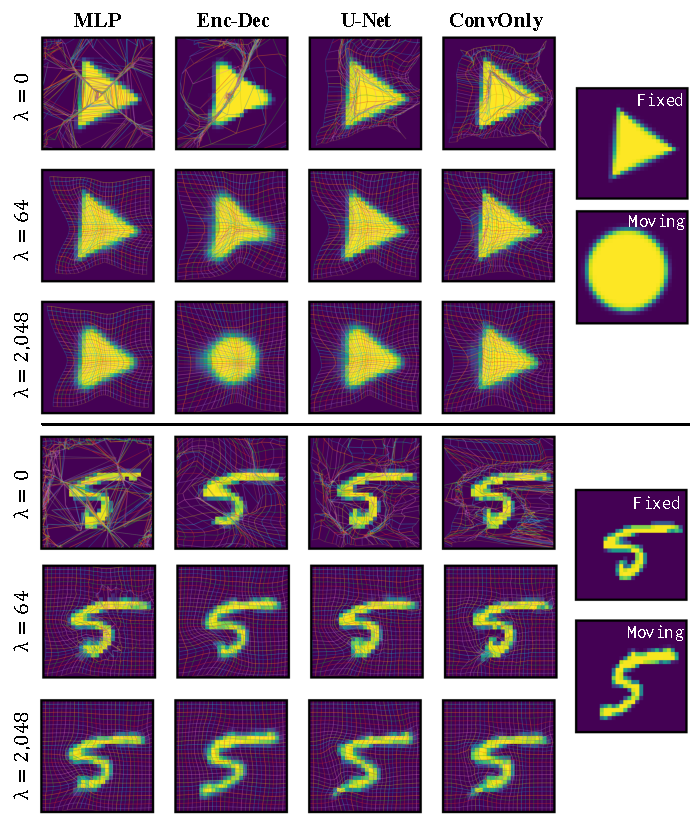
\includegraphics[width=0.97\columnwidth]{TrianglesFivesCombined.pdf}
  % \resizebox{\columnwidth}{!}{
  % \begin{tabular}{c}
  %   \includegraphics[width=1.0\columnwidth]{Foobar} \\
  %   \includegraphics[width=1.0\columnwidth,angle=-90]{Triangles-2}
  % \end{tabular}
  % }
%\includegraphics[width=160pt]{tri_quant.png}
%\includegraphics[width=160pt]{mnist_quant.png}

\caption{Comparison of networks as a function of $\lambda$. \textbf{U-Net} and \textbf{MLP} show the best performance due to their ability to capture long and short range dependencies. \textbf{Enc-Dec} and \textbf{ConvOnly}, which capture only long range and only short range dependencies, resp., also learn regular maps, but for a narrower range of $\lambda$. In all cases, maps become smooth for sufficiently large $\lambda$. Best viewed zoomed.} \label{fig:registration_across_architectures}
\vspace{-0.2cm}
\end{figure}

Sec.~\ref{subsec:imperfect_inverse_consistency} illustrated that approximate inverse consistency yields regularization effects which translate to regularity for network predictions, as networks will, in general, not achieve perfect inverse consistency. A natural next question to ask is ``how much the results depend on a particular architecture''? To this end, we assess four different network types, focusing on MNIST and the triangles \& circles data. We report two measures on held-out images: the \emph{Dice score} of pixels with intensity greater than $0.5$, and the mean number of \emph{folds}, \ie, pixels where the volume form $\mathrm{d}V$ of $\Phi$ is negative.

%The first question we address is whether the regularity of the transforms produced by our technique is enforced by the inverse consistency loss, or if the observed regularity is, in fact, an artifact of the network design.  
%If an experimenter combines our loss with their architecture, are they likely to obtain good results for an appropriate $\lambda$? 
%To that end, we use the same loss with four neural network architectures and two different toy datasets: all the numbers "5" from \texttt{MNIST}, and a collection of 6,000 triangles and circles. 

% \todo[inline]{I think it would also be good to somewhere at the beginning describe the different network architectures you used. Some of this material should likely go into supplementary material. Also, do you mean fully connected when you say dense?}

\vskip0.5ex
One hypothesis as to how network design could drive smoothness %-- which could invalidate our claim that transform regularity is driven by the loss --
would be that smoothness is induced by convolutional layers (which can implement a smoothing kernel). 
If this were the case, we would expect the \textbf{MLP} to produce irregular maps with a high number of folds. Vice versa, since the \textbf{MLP} has no spatial prior, obtaining smooth transforms would indicate that smoothness is promoted by the loss itself. The latter is supported by Fig.~\ref{fig:registration_across_architectures}, showing regular maps even for the \textbf{MLP} when $\lambda$ is sufficiently large. Note that $\lambda=0$ in Fig.~\ref{fig:registration_across_architectures} corresponds to an unregularized MSE solution, as discussed in Sec.~\ref{subsection:regularization_thoughts_and_sorting}; maps are, as expected, highly irregular and regularization via inverse consistency is clearly needed.

% see Fig.~\ref{fig:registration_across_architectures}), indicating that the transform is regularized by the loss function as opposed to any spatial prior in the network.  
%if we obtain smooth transforms from a dense network then we know that the smoothness is coming from the loss
% the regularity we observe in the transform is driven by the loss function, would be that the smoothness we see in U-Net results actually comes from the convolution operator in our neural network, which can implement a smoothing kernel. If this were the case, we would expect a dense neural network trained on our loss to produce transforms with a high number of folds, or some other sort of qualitative deficiency. Alternatively, since a dense network has no spatial prior, if we see smooth transforms from a dense network then we know that the smoothness is coming from the loss. To test this, we train a dense (fully connected) neural network on our 2-D datasets. We obtain smooth results (see Fig.~\ref{fig:registration_across_architectures}), indicating that the transform is regularized by the loss function as opposed to any spatial prior in the network.  

\vskip0.5ex
A second hypothesis is that regularity results from a \emph{bottleneck} structure within a network, \eg, a \textbf{U-Net}. In fact, Bhalodia \etal~\cite{bhalodia19} show that autoencoders tend to yield smooth maps. To assess this hypothesis, we focus on the \textbf{Enc-Dec} and \textbf{ConvOnly} type networks; the former has a bottleneck structure, while the latter does not.
Fig.~\ref{fig:registration_across_architectures} shows some support for the hypothesis that a bottleneck promotes smooth maps: for a specific $\lambda$, \textbf{Enc-Dec} appears to have more strongly regularized outputs compared to \textbf{U-Net}, with \textbf{ConvOnly} being the most irregular.
%the Encoder-Decoder appears to have intensely regularized outputs %compared to the U-Net, while the pure convolution (with no upsampling %or downsampling) network has more irregular outputs than the U-Net. 
Yet, higher values of $\lambda$ (\eg, 1,024 or 2,048) for \textbf{ConvOnly} yield equally smooth maps. Overall, a bottleneck structure does have a regularizing effect, but regularity can also be achieved by appropriately weighing the inverse consistency loss (see Tab.~\ref{tab:registration_across_architectures}).

\vskip0.5ex
\emph{In summary, our experiments indicate that the regularizing effect of inverse consistency is a robust property of the loss, and should generalize well across architectures.}

% As a result, the ideal value of $\lambda$ appears to vary with network architecture, in these extreme cases all the way from 64 for the autoencoder to 2048 or 1024 for the purely convolutional network. However, for appropriate values of $\lambda$ all three networks work.
% \todo[inline]{Wasn't the argument that one can use a wide range of $\lambda$'s and hence these networks are easy to tune. This seems to be contradicted by what you say above.}

% To test this we create two networks, one by removing the downsampling and upsampling layers of the U-Net, leaving a network composed only of full resolution convolutions, and another where we strip out the skip connections, leaving an Encoder-Decoder. Fig.~\ref{fig:registration_across_architectures} shows some support for the hypothesis that a bottleneck has a smoothing effect: the Encoder-Decoder appears to have intensely regularized outputs compared to the U-Net, while the pure convolution (with no upsampling or downsampling) network has more irregular outputs than the U-Net. As a result, the ideal value of $\lambda$ appears to vary with network architecture, in these extreme cases all the way from 64 for the autoencoder to 2048 or 1024 for the purely convolutional network. However, for appropriate values of $\lambda$ all three networks work.
% \todo[inline]{Wasn't the argument that one can use a wide range of $\lambda$'s and hence these networks are easy to tune. This seems to be contradicted by what you say above.}

%The third hypothesis we investigated is that the smoothness comes from the texture of the data, because a unique smooth map aligns each bump and crag in the optimal way~\cite{niethammer2019metric}. The second dataset of filled shapes was included to check whether this was the case, with large textureless regions inside the shapes. Fig.~\ref{fig:registration_across_architectures} illustrates that in these textureless regions inverse consistency is still sufficient to force a neural network to output a smooth transform. 

%\subsection{ Comparison to direct optimization of $\Phi_{AB}$ / $\Phi_{BA}$}
%% \todo[inline]{The following sentence is a bit complex and should be simplified. Need to read the paper to do this. Or Hastings can you do it, as you read this paper in more detail?}
%%Bhalodia et al.~\cite{bhalodia19} found that registration neural networks operating on a population of images, when forced to match the output of another neural network while passing the registration information through a bottleneck layer, necessarily output transforms on a submanifold of the space of all transforms. Further, they found that transforms in that submanifold are smooth. If this effect is driving the smoothness of our results, we expect that our loss should not produce smooth results when the transforms themselves are optimized instead of network weights.
%In this experiment, we compare our approach to directly optimizing vectors of the \emph{deformation field}, as typically done in traditional pairwise image registration. We specifically focus on the synthetic triangles \& circles dataset and train a \textbf{U-Net} architecture with the inverse consistency loss and $\lambda=2048$. 
%%We investigate aligning triangles and circles, but this time as outlines instead of filled in and at a resolution of 128 x 128 instead of 28 x 28. We train a U-Net architecture with $\lambda = 2048$ on this dataset and loss. We compare it to optimizing vectors of the deformation field directly, as in traditional pairwise image registration. 
%As can be seen from Fig.~\ref{fig:high_res_shape_outlines} (columns 4 \& 7), both approaches produce invertible transforms, since, in each case, the composition of $\Phi^{AB}$ and $\Phi^{BA}$ is close to the identity.
%%Both 
%% to produce invertible transforms, as can be seen in columns 4 and 7 of Fig.~\ref{fig:high_res_shape_outlines}, since in each case the composition of $\Phi_{AB}$ and $\Phi_{BA}$ is close to the identity. 
%  However, training the network with the proposed inverse consistency loss yields smooth deformations, while direct optimization of the deformation field produces very ragged deformations. While invertible, such deformations are not semantically meaningful. This provides strong empirical evidence that the inverse consistency loss exerts implicit regularization applied to the gradient, resulting from the neural network's uncertainty about how it will behave with swapped inputs 
%  (especially in textureless areas). When this uncertainty is removed by always using the same pair of images, the implicit gradient penalty vanishes.
%This also elucidates why inverse consistency has not appeared in the classical image registration literature as a replacement for more complicated smoothness constraints. The proposed technique only solves the aperture problem in the presence of a population, and so is not suitable for direct optimization.

%% \todo[inline]{Agree! The population aspect is, to me, the key factor for smoothness ... as the data acts as an implicit regularizer. Also, it might be due to SGD, e.g., as it is hypothesized that SGD prefers ``simple'' solutions, see, e.g., 
%  https://arxiv.org/pdf/1909.12051.pdf}


%    \centering
%    \begin{tabular}{c c c c}
%       Image A & With Noise & Without Noise & Image B \\
%    \end{tabular}
%    \includegraphics[width=1\columnwidth]{noise_small.png}
%    \caption{Result of directly optimizing the displacement maps $D^{AB}$ and $D^{BA}$ to minimize our loss, with and without noise added during the computation of $Phi$ from $D$. When noise is added to the maps, regularized transforms are produced, while without noise no regularization occurs. No neural network is involved in this experiment.}
%    \label{fig:regularizing_via_noise}
%\end{figure}

\subsection{Performance for 3D image registration}

% \todo[inline]{Here you also give some details on batchsize etc., but you don't do this for any of the other experiments. Would be good to have a section to summarize all of these different network settings for all the experiments. Could also go partially into the supplementary material.}

For experiments on real data, we focus on the 3D OAI dataset. To demonstrate the versatility of the advocated inverse consistency loss in promoting map regularity, we refrain from affine pre-registration (as typically done in earlier works) and simply compose \mn{the maps of} \emph{multiple U-Nets} instead. In particular, we compose up to four U-Nets \mn{as follows:} A composition of two U-Nets is initially trained on low-resolution image pairs. Weights are then frozen and this network is composed with a third U-Net, trained on high-resolution image pairs. This network is then optionally frozen and composed with a fourth U-Net, again trained on high-resolution image pairs. During the training of this multi-step approach, the weighting of the inverse consistency loss is gradually increased. We train using ADAM \cite{Kingma15a} with a batch size of 128 in the low-res. stage, and a batch size of 16 in the high-res. stage. MSE is used as image similarity measure.

\vskip0.5ex
We compare our approach, \textcolor{ggreen}{InverseConsistentNet} \mn{(\texttt{ICON})}, against the methods of \cite{shen2019networks}, in terms of (1) cartilage Dice scores between registered image pairs~\cite{AmbellanTackEhlkeetal.2018} (based on manual segmentations) and (2) the number of folds. The segmentations are not used during training and allow quantifying if the network yields semantically meaningful registrations. Tab.~\ref{tab:oai_results} lists the corresponding results, Fig.~\ref{fig:teaser} shows several example registrations. Unlike the other methods in Tab.~\ref{tab:oai_results}, except where explicitly noted, \mn{\texttt{ICON} does not require affine pre-registration. Since affine maps are inverse consistent, they are not penalized by our method.}
%, as the deformation can capture the affine component,
Notably, despite its simplicity, \texttt{ICON} yields performance (in terms of Dice score \& folds) comparable to more complex, explicitly regularized methods. We emphasize that our objective is not to outperform existing techniques, but to present evidence that regular maps can be learned \emph{without} carefully tuned regularizers.


% Tab.~\ref{tab:registration_across_architectures} indicated good performance across architectures (for appropriate $\lambda$'s), but in particular for the \textbf{MLP}. 
% An \textbf{MLP} is, of course, not possible in 3D. 
% Hence, we train a 3D \textbf{U-Net} instead. 
% To compete with other state-of-the-art registration techniques (\cf \cite{shen2019networks}), we rely on a more expressive architecture, composed of multiple U-Net steps and a training schedule for $\lambda$ (see supp. mat. for details). We train using SGD with a batch-size of 128 during low-resolution pre-training and a batch-size of 8 during training with high-resolution images.

% We use SSD image similarity, and use a batch size of 128 during low resolution pretraining, and a batch size of 8 during the final high resolution training. We use a training schedule for lambda, ending on 3200, as described in more detail in the supplementary material. Training takes approximately 4 days on 4 RTX 2080s. We compare cartilage Dice scores between registered image pairs~\cite{AmbellanTackEhlkeetal.2018} based on manual segmentations. These segmentations are not used during training and allow quantifying if the network yields semantically meaningful registrations. Tab.~\ref{tab:oai_results} shows the good performance of our approach. Notably, unlike the other methods in the table except where explicitly noted, our technique has no affine pre-registration, as the deformation can capture the affine component since affine maps are inverse consistent, and hence not penalized by our method.

% During this process we determined one unfortunate property of our loss function, which is that it demands a large batch size to capture large deformations, as with a batch size less than 128 the network did not capture the full range of shifts and warps present in the OAI dataset. For this reason, we  heavily downsampled the input in order to fit batches into VRAM: the original OAI images are 384 x 384 x 160, and the registration methods we compared to were all able to run at 192 x 192 x 80, while our network accepted images 96 x 96 x 40. For this reason, we upsample the transforms produced by our network to 192 x 192 x 80 so that our results can be directly compared with these other methods. 

\vskip0.5ex
\emph{In summary, using the proposed inverse consistency loss yields (1) competitive Dice scores, (2) acceptable folds, and (3) fast performance.}

%reduced computation time (as testing just boils down to a forward pass through the model). 

% \begin{figure}
%   \centering
%   \includegraphics[width=0.32\columnwidth]{oai-a-trimmed.png}\hfill
%   \includegraphics[width=0.32\columnwidth]{oai-warped-b-trimmed.png}\hfill
%   \includegraphics[width=0.32\columnwidth]{oai-b-trimmed.png}
%   % \resizebox{\columnwidth}{!}{
%   % \begin{tabular}{ccc}
%   %   \includegraphics[width=0.335\columnwidth]{oai-a-trimmed.png} &
%   %   \includegraphics[width=0.335\columnwidth]{oai-warped-b-trimmed.png} &
%   %   \includegraphics[width=0.335\columnwidth]{oai-b-trimmed.png}
%   % \end{tabular}
%   % }
%   \caption{Example OAI registration result generated by our network. \emph{Left to right}: fixed, warped moving, and moving image. The warped moving image is visually very similar to the fixed image; the transformation grid (colored) is, as desired, smooth.}
%   %OAI data is challenging for a registration technique because of the large variation in size and shape of the joint and the framing of the MR images.}
%     \label{fig:oai_example}
% \end{figure}


\begin{table}
\begin{small}
\centering
\resizebox{\columnwidth}{!}{%
\begin{tabular}{lllll}
\toprule
\textbf{Method} &  $\mathcal{L}_{sim}$ & \textbf{Dice} & \textbf{Folds} & \textbf{Time} [s]\\
\midrule
Demons & MSE & 63.47 & 19.0 & 114\\
SyN & CC & 65.71 & 0 & 1330\\
NiftyReg & NMI & 59.65 & 0 & 143\\
NiftyReg & LNCC & 67.92 & 203 & 270\\
vSVF-opt & LNCC & 67.35 & 0 & 79\\
Voxelmorph (w/o affine) & MSE & 46.06 & 83 & 0.12\\
Voxelmorph & MSE & 66.08 & 39.0 & 0.31\\
AVSM (7-Step Affine, 3-Step Deformable) & LNCC & 68.40 & 14.3 & 0.83\\
\midrule
\textcolor{ggreen}{\texttt{ICON}} (2 step \nicefrac{1}{2} res., 2 step full res., w/o affine) & MSE & 68.29 & 118.4 & 1.06\\
\textcolor{ggreen}{\texttt{ICON}} (2 step \nicefrac{1}{2} res., 1 step full res., w/o affine) & MSE & 66.16 & 169.4  & 0.57 \\
\textcolor{ggreen}{\texttt{ICON}} (2 step \nicefrac{1}{2} res., w/o affine) & MSE & 59.36 & 49.35  & 0.09 \\
\bottomrule 
\end{tabular}
}
\caption{Comparison of \textcolor{ggreen}{\texttt{ICON}} against the methods in \cite{shen2019networks}, on cross-subject registration for OAI knee images.\label{tab:oai_results}}
\vspace{-0.2cm}
\end{small}
\end{table}

\section{Limitations, future work, \& open questions}
\label{sec:future_work}

Several questions remain and there is no shortage of theoretical/practical directions, some of which are listed next.

%For example, exploring different similarity measures (both classical measures, such as mutual information or localized normalized cross correlation, as well as measures based on deep features) could further improve our approach.
%Convergence could likely be accelerated by implementing a multi-scale strategy and accuracy might improve by multi-step extensions.
%As we only regularize via inverse consisteny, extensions to piecewise diffeomorphic formulations seem conceivable.

\vskip0.5ex
\noindent
\textbf{Network architecture \& optimization.} Instead of specifying a spatial regularizer, we now specify a network architecture. While our results suggest regularizing effects for a variety of architectures, we are still lacking a clear understanding of how network architecture and numerical optimization influence solution regularity.

\vskip0.5ex
\noindent
{\bf Diffemorphisms at test time.} We simply encourage inverse consistency via a quadratic penalty. Advanced numerical approaches (\eg, augmented Lagrangian methods~\cite{nocedal2006numerical}) could more strictly enforce inverse consistency during \emph{training}. Our current approach is only \emph{approximately diffeomorphic} at test time. To guarantee diffeomorphisms, one could explore combining inverse consistency with fluid deformation models~\cite{holden2007review}. These have been used for deep registration networks~\cite{yang2017quicksilver,yang2016fast,shen2019networks,shen2019region,dalca2018unsupervised} combined with explicit spatial regularization. We would simply predict a velocity field and obtain the map via integration. By using our loss, sufficiently smooth velocity fields would likely emerge. Alternatively, one could use diffeomorphic transformation parameterizations by enforcing positive Jacobian determinants~\cite{shu2018deforming}.

\vskip0.5ex
\noindent
{\bf Multi-step.} Our results show that using a multi-step estimation approach is beneficial; successive networks can refine deformation estimates and thereby improve registration performance. What the limits of such a multi-step approach are (i.e., when performance starts to saturate) and how it interacts with deformation estimates at different resolution levels would be interesting to explore further. 

\vskip0.5ex
\noindent
{\bf Similarity measures.} For simplicity, we only explored MSE. NCC, local NCC, and mutual information would be natural choices for multi-modal registration. In fact, there are many opportunities to improve registrations \eg using more discriminative similarity measures based on network-based features, multi-scale information, or side-information during training, \eg, segmentations or point correspondences.

% We now use a multi scale strategy, and so this doesn't belong in future work
%\vskip0.5ex
%\noindent
%{\bf Multi-scale strategy.} Convergence could likely be accelerated by a multi-scale strategy and accuracy might improve by multi-step extensions~\cite{shen2019networks}.
%
% \vskip0.5ex
% \noindent
% {\bf Piecewise diffeomorphisms.} Not all maps are diffeomorphic and more general transformation models, such as piecewise diffeomorphisms should be explored. Those could, \eg, be achieved via  inverse consistency on separate subregions.
% %As we no longer use an explicit spatial regularizer such models are expected to be much easier to formulate.

\vskip0.5ex
\noindent
{\bf Theoretical investigations.} It would be interesting to establish how regularization by inverse consistency relates to network capacity, expressiveness, and generalization. Further, establishing a rigorous theoretical understanding of the regularization effect due to the data \emph{population} and its link with inverse consistency would be important.

\vskip0.5ex
\noindent
{\bf General inverse consistency.} Our work focused on spatial correspondences for registration, but the benefits of inverse consistency regularization are likely much broader. For instance, its applicability to general mapping problems (\eg, between feature vectors) should be explored.


% \begin{itemize}[itemsep=2pt, topsep=0pt,parsep=0pt,partopsep=0pt,leftmargin=*]
% \item {\it Network architecture \& Optimization}: Instead of specifying a spatial regularizer, we now specify a network architecture. While our results suggest regularizing effects for a variety of network architectures, we are still lacking a clear understanding of how network architecture and numerical optimization influence solution regularity.
% \item {\it Diffemorphisms at test time}: We simply encourage inverse consistency via a quadratic penalty. Advanced numerical approaches (e.g., augmented Lagrangian methods~\cite{nocedal2006numerical}) could more strictly enforce inverse consistency during \emph{training}. Note that our current approach is only \emph{approximately diffeomorphic} at test time. To guarantee diffeomorphisms one could explore combining inverse consistency with fluid deformation models~\cite{holden2007review}. These have been used for deep registration networks~\cite{yang2017quicksilver,yang2016fast,shen2019networks,shen2019region,dalca2018unsupervised} combined with explicit spatial regularization. We would simply predict a velocity field and obtain the map via integration. By using our inverse consistency loss,  sufficiently smooth velocity fields would likely emerge. Alternatively, we could use diffeomorphic transformation parameterizations by enforcing positive Jacobian determinants~\cite{shu2018deforming}.
% \item {\it Similarity measures}: For simplicity, we only explored SSD. NCC, local NCC, and mutual information would be natural choices for multi-modal registration. In fact, there are many opportunities to improve registrations by using more discriminative similarity measures based on network-based features, or side-information during training, e.g., segmentations or point correspondences.
% \item {\it Multi-scale strategy}: Convergence could likely be accelerated by a multi-scale strategy and accuracy might improve by multi-step extensions~\cite{shen2019networks}.
% \item {\it Piecewise diffeomorphisms}: Not all maps are diffeomorphic and more general transformation models, such as piecewise diffeomorphisms should be explored. Those could likely be achieved by imposing inverse consistency on separate subregions.
% %As we no longer use an explicit spatial regularizer such models are expected to be much easier to formulate.
% \item {\it Theoretical investigations}: It would be interesting to establish how regularization by inverse consistency relates to network capacity, expressiveness, and generalization. Further, establishing a rigorous theoretical understanding of the regularization effect due to the data \emph{population} and its link with inverse consistency would be important,
% \item {\it General inverse consistency}: Our work focused on spatial correspondences for registration, but the benefits of inverse consistency regularization are likely much broader. E.g., its applicability to general mapping problems (e.g., between feature vectors) should be explored.
%  \end{itemize}

%

%\begin{itemize}[noitemsep,topsep=0pt,parsep=0pt,partopsep=0pt,leftmargin=*]
%\item {\it Network architecture and optimization}: Classic nonparametric registration approaches make use of a similarity measure and a regularizer penalizing spatial derivatives. We have now shifted our focus to weak regularization via inverse consistency and the choice of a network architecture. It would be interesting to further explore how network architecture affects solution regularity and what role the chosen optimization strategy plays.
%\item {\it Enforcing diffemorphisms at test time}: We use a relatively na\"ive way of enforcing inverse consistency via a quadratic penalty as we targeted a simple formulation. But more advanced approaches to encourage or enforce inverse consistency could easily be explored. For example, one could use an augmented Lagrangian strategy for inverse consistency~\cite{nocedal2006numerical}. This would increase training time, but would likely result in even greater insensitivity with respect to the choice of a penalty parameter. Of course, none of the methods which encourage inverse consistency via a loss during training will assure inverse consistency at testing time. This is why we talk about ``approximately diffeomorphic'' registration for our proposed approach. However, it would be straightforward to combine the approach with a fluid model~\cite{holden2007review}. Such transformation models have also been explored for deep registration networks~\cite{yang2017quicksilver,yang2016fast,shen2019networks,shen2019region,dalca2018unsupervised} and typically use a regularizer penalizing spatial derivatives on the velocity field. Hence, we could simply predict this velocity field and use our inverse consistency loss in the same way. The only difference would be that the transformation map would be obtained via numerical integration. Another alternative would be to use a parameterization which will be diffeomorphic by construction (by assuring that the determinant of Jacobian stays positive) as done in~\cite{shu2018deforming}.
%\item {\it Alternative similarity measures}: For simplicity we have only explored a basic SSD similarity measures here. NCC, local NCC, and mutual information would be natural choices for multi-modal registration. However, there are much richer opportunities to explore similarity measures based on feature embeddings of the network (to capture more complex and descriptive image information) or similarity measures based on point-clouds or surfaces (for example, using similarity measures motivated by optimal mass transport theory), or using side-information such as segmentations at training time. Such advanced similarity measures might result in improved correspondences as they can be significantly more discriminative with respect to local image structure.
%\item {\it Multi-scale strategy}: Convergence could likely be accelerated by implementing a multi-scale strategy and accuracy might improve by multi-step extensions.
%\item {\it Piecewise diffeomorphic transformations}: In practice, not all transformations can be assumed to be diffeomohpic. Piecewise diffeomorphic transformation would be interesting to explore and transformations which might no longer be one-to-one everywhere (for example when two tissues separate during deformation). It would be interesting to see how such methods could be formulated and how they might intersect with registration work related to occlusion modeling in computer vision.
%\item {\it Theoretical investigations}: It would be highly interesting to theoretically investigate what causes the desirable smoothness properties and how they relate to network capacity, expressiveness, and generalization.
%\end{itemize}


\section{Conclusion}
\label{sec:conlusion}

We presented a deliberately simple deep registration model which generates approximately diffeomorphic maps by regularizing via an inverse consistency loss. We theoretically analyzed why inverse consistency leads to spatial smoothness and empirically showed the effectiveness of our approach, yielding \mn{competitive} %state-of-the-art
3D registration performance. 

\vskip1ex
Our results suggest that simple deep registration networks might be as effective as more complex approaches which require substantial hyperparameter tuning and involve choosing complex transformation models. As a wide range of inverse consistency loss penalties lead to good results, only the desired similarity measure needs to be chosen and extensive hyperparameter tuning can be avoided. This opens up the possibility to easily train extremely fast custom registration networks on given data. Due to its simplicity, ease of use, and computational speed, we expect our approach to have significant practical impact. We also expect that inverse consistency regularization will be useful for other tasks, which should be explored in future work.
%\clearpage

% Acknowledgements should only appear in the accepted version.

\opt{for_gig,icml_accepted,iccv_submission}
{
  \section*{Acknowledgments}

  This research was supported in part by Award Number R21-CA223304 from the National Cancer Institute and Award Number 1R01-AR072013 from the National Institute of Arthritis and Musculoskeletal and Skin Diseases of the National Institutes of Health. It was also supported by an MSK Cancer Center Support Grant/Core Grant P30 CA008748 and by the National Science Foundation (NSF) under award number NSF EECS-1711776. It was also supported by the Austrian Science Fund (FWF): project FWF P31799-N38 and the Land Salzburg (WISS 2025) under project numbers 20102- F1901166-KZP and 20204-WISS/225/197-2019. The content is solely the responsibility of the authors and does not necessarily represent the official views of the NIH or the NSF. The authors have no conflicts of interest.
}
  
\opt{for_gig,icml_submission}
{
  \bibliographystyle{icml2021}
  \bibliography{mybibliography}
}
\opt{iccv_submission}
    {
      
      {\small
        \bibliographystyle{ieee_fullname}
        \bibliography{mybibliography}
      }
    }

\end{document}


% This document was modified from the file originally made available by
% Pat Langley and Andrea Danyluk for ICML-2K. This version was created
% by Iain Murray in 2018, and modified by Alexandre Bouchard in
% 2019 and 2021. Previous contributors include Dan Roy, Lise Getoor and Tobias
% Scheffer, which was slightly modified from the 2010 version by
% Thorsten Joachims & Johannes Fuernkranz, slightly modified from the
% 2009 version by Kiri Wagstaff and Sam Roweis's 2008 version, which is
% slightly modified from Prasad Tadepalli's 2007 version which is a
% lightly changed version of the previous year's version by Andrew
% Moore, which was in turn edited from those of Kristian Kersting and
% Codrina Lauth. Alex Smola contributed to the algorithmic style files.

%%%%%%%% ICML/ICCV 2021 EXAMPLE LATEX SUBMISSION FILE %%%%%%%%%%%%%%%%%

\documentclass[10pt,onecolumn,letterpaper]{article} % comment out for ICCV style paper
%\documentclass[onecolumn]{article} % comment out for NeurIPS style paper

\usepackage{etex}
\usepackage{todonotes}

% MN: to create different versions
%\usepackage[icml_submission]{optional}
%\usepackage[icml_accepted]{optional}
%\usepackage[for_gig]{optional}
\usepackage[iccv_submission]{optional}

\opt{iccv_submission}{
  \usepackage{iccv_supplementary}
  \usepackage{times}
  \usepackage{epsfig}
  \usepackage{graphicx}
  \usepackage{amsmath}
  \usepackage{amssymb}
  \usepackage{listings} 
  % Include other packages here, before hyperref.
  
  % If you comment hyperref and then uncomment it, you should delete
  % egpaper.aux before re-running latex.  (Or just hit 'q' on the first latex
  % run, let it finish, and you should be clear).
  \usepackage[pagebackref=true,breaklinks=true,letterpaper=true,colorlinks,bookmarks=false]{hyperref}
  
  \iccvfinalcopy % *** Uncomment this line for the final submission
  
  \def\iccvPaperID{10828} % *** Enter the ICCV Paper ID here
  \def\httilde{\mbox{\tt\raisebox{-.5ex}{\symbol{126}}}}

  % Pages are numbered in submission mode, and unnumbered in camera-ready
  \ificcvfinal\pagestyle{empty}\fi


}

\opt{icml_submission,for_gig}{
  \usepackage{graphicx}
  \usepackage{amsmath}
  \usepackage{amssymb}
  \usepackage[colorlinks=true,linkcolor=blue,citecolor=blue]{hyperref}
  \usepackage[table]{xcolor}
}



% Recommended, but optional, packages for figures and better typesetting:
\usepackage{microtype}
\usepackage{subfigure}
\usepackage{booktabs} % for professional tables

\usepackage{enumitem}

\usepackage{amsfonts}

\usepackage{tikz}

\usetikzlibrary{arrows.meta, % if the figure contains arrow-tips
                bending,     % arrow tips on arcs are "bent," i.e., deformed a bit
                patterns     % if the figure contains pattern fills
               }

\usetikzlibrary{spy}
\usetikzlibrary{arrows,shapes,automata,backgrounds,petri,positioning}
\usetikzlibrary{decorations.pathmorphing}
\usetikzlibrary{decorations.shapes}
\usetikzlibrary{decorations.text}
\usetikzlibrary{decorations.fractals}
\usetikzlibrary{decorations.footprints}
\usetikzlibrary{shadows}


\renewcommand\floatpagefraction{.99}
\renewcommand\topfraction{.99}
\renewcommand\bottomfraction{.99}
\renewcommand\textfraction{.01}   
\setcounter{totalnumber}{50}
\setcounter{topnumber}{50}
\setcounter{bottomnumber}{50}

%\setlength{\textfloatsep}{0.25\baselineskip plus 0.2\baselineskip minus 0.5\baselineskip}

\setlength{\textfloatsep}{1.25\baselineskip plus 0.2\baselineskip minus 0.5\baselineskip}

\DeclareMathOperator{\id}{Id}
\newcommand{\fxpsi}{\Phi_{\theta}^{BA}}
\newcommand{\fxvarphi}{\Phi_{\theta}^{AB}}
\newcommand{\fxpsivarepsilon}{\Phi_{\theta \varepsilon}^{BA}}
\newcommand{\fxvarphivarepsilon}{\Phi_{\theta \varepsilon}^{AB}}
\graphicspath{{figs/}}

\newcommand{\mn}[1]{{\color{blue}{#1}}}
\newcommand{\mnl}[1]{{\color{red}{$\leftarrow$~#1}}}
\newcommand{\mnr}[1]{{\color{red}{#1~$\rightarrow$}}}
\newcommand{\zp}[1]{{\color{blue}{#1}}}
\newcommand{\fx}[1]{{\color{magenta}{#1}}}

% hyperref makes hyperlinks in the resulting PDF.
% If your build breaks (sometimes temporarily if a hyperlink spans a page)
% please comment out the following usepackage line and replace
% \usepackage{icml2021} with \usepackage[nohyperref]{icml2021} above.
%\usepackage{hyperref}

% Attempt to make hyperref and algorithmic work together better:
\newcommand{\theHalgorithm}{\arabic{algorithm}}

\opt{icml_submission}{
% Use the following line for the initial blind version submitted for review:
\usepackage{icml2021}

\usepackage{setspace}
\usepackage[labelfont={bf,small},font={small,stretch=1.1}]{caption}
%\usepackage{subcaption}

\usepackage[colorinlistoftodos,prependcaption,textsize=tiny]{todonotes}
}

\opt{icml_accepted}{
% If accepted, instead use the following line for the camera-ready submission:
  \usepackage[accepted]{icml2021}
}

\opt{for_gig}{
  \usepackage[accepted]{icml2021_unpublished_draft}
  \usepackage[colorinlistoftodos,prependcaption,textsize=tiny,disable]{todonotes}
  % disable todos
  %\usepackage[colorinlistoftodos,prependcaption,textsize=tiny,disable]{todonotes}
}
\pagenumbering{roman}
\begin{document}

\sloppy

\opt{iccv_submission}{
  %%%%%%%%% TITLE
\title{ICON: Supplementary Material}

\author{Hastings Greer\\
  Department of Computer Science\\
UNC Chapel Hill, USA\\
{\tt\small tgreer@cs.unc.edu}
% For a paper whose authors are all at the same institution,
% omit the following lines up until the closing ``}''.
% Additional authors and addresses can be added with ``\and'',
% just like the second author.
% To save space, use either the email address or home page, not both
\and
Roland Kwitt\\
Department of Computer Science\\
University of Salzburg, Austria\\
{\tt\small Roland.Kwitt@sbg.ac.at}
\and
Fran\c{c}ois-Xavier Vialard\\
LIGM, Universit\'e Gustave Eiffel, France\\
{\tt\small francois-xavier.vialard@u-pem.fr}
\and
Marc Niethammer\\
 Department of Computer Science\\
UNC Chapel Hill, USA\\
{\tt\small mn@cs.unc.edu}
}

\maketitle
% Remove page # from the first page of camera-ready.
\ificcvfinal\thispagestyle{empty}\fi
}
\thispagestyle{plain}
\pagestyle{plain}

\opt{for_gig,icml_submission}{

% The \icmltitle you define below is probably too long as a header.
% Therefore, a short form for the running title is supplied here:
%\icmltitlerunning{Inverse Consistency is Almost All You Need}
\icmltitlerunning{Learning Regular Maps Through Inverse Consistency}
  
\onecolumn[
%\icmltitle{Inverse Consistency is All You Need \\ -- for Image Registration}
\icmltitle{Learning Regular Maps Through Inverse Consistency}

\icmlsetsymbol{equal}{*}

\begin{icmlauthorlist}
\icmlauthor{Hastings Greer}{unc}
\icmlauthor{Roland Kwitt}{salzburg}
\icmlauthor{Fran\c{c}ois Xavier-Vialard}{upem}
\icmlauthor{Marc Niethammer}{unc}
\end{icmlauthorlist}

\icmlaffiliation{unc}{Department of Computer Science, University of North Carolina at Chapel Hill, USA}
\icmlaffiliation{salzburg}{Department of Computer Science, University of Salzburg, Austria}
\icmlaffiliation{upem}{LIGM, Universit\'e Gustave Eiffel, France}

\icmlcorrespondingauthor{Hastings Greer}{tgreer@cs.unc.edu}

\icmlkeywords{Deep Learning, Image Registration, Inverse Consistency}

\vskip 0.3in
]

%\printAffiliationsAndNotice{}  % leave blank if no need to mention equal contribution
\printAffiliationsAndNotice{\icmlEqualContribution} % otherwise use the standard text.
}

\sloppy

%\onecolumn
\section*{Introduction}
We cover these topics in the supplementary material that did not fit into the main manuscript:
\begin{itemize}
\item We retrace the proof of the $H^1$ regularizing property of approximate inverse consistency in greater detail.
\item We specify all details of the neural network architectures used in the manuscript's experiments, including number of features, number of layers, training proceedure, etc.
\end{itemize}

\section{Detailed proof of the regularizing effect of inverse consistency}

This section details our derivation for the smoothness properties emerging from approximate inverse consistency. 

%\subsection{Smoothness via approximate inverse consistency} 

%We now give arguments for the regularizing properties of approximate inverse consistency in the context of pairwise image registration.
Denote by $\fxvarphi(x)$ the output map of a network for images $(I^A,I^B)$ and by $\fxpsi(x)$ the output map between $(I^B,I^A)$
%\todo{FX, I put this back in. There was somehow something missing in the text.}.
%FX: ok
%In practice, this map is only defined at grid points, but we extend it to the full domain by interpolation. %However, our arguments apply quite independently of how the maps are actually computed.
%Inverse consistency by itself does not prevent discontinuous solutions, we propose to use approximate inverse consistency to favor $C^0$ solutions. 
%We now show that once diffeomorphic solutions have been favored, an implicit $H^1$ regularization emerges from the introduction of the noise.
Recall that we add two independent spatial white noises $n_1(x),~n_2(x)\in\mathbb{R}^N$ ($x \in [0,1]^N$ with $N = 2$ or $N = 3$ the dimension of the image)
%$n_1(i,x),n_2(i,x)$
%($i = 1,\ldots,N$; $x \in [0,1]^N$ with $N = 2$ or $N = 3$ the dimension of the image)
of variance $1$ for each spatial location to the two output maps and define $\fxvarphivarepsilon(x) := \fxvarphi(x) + \varepsilon n_1(\fxvarphi(x))$ and $\fxpsivarepsilon(x) := \fxpsi(x) + \varepsilon n_2(\fxpsi(x))$ with $\varepsilon$ a positive parameter.
We consider the following loss
\begin{multline}\label{EqLossSymmetric2}
    \mathcal{L} =\lambda \left( \| \fxvarphivarepsilon \circ \fxpsivarepsilon - \operatorname{Id} \|^2_2 + \| \fxpsivarepsilon \circ \fxvarphivarepsilon - \operatorname{Id} \|^2_2 \right) + \| I^A \circ \fxvarphi - I^B \|^2_2 + \| I^B \circ \fxpsi  - I^A \|^2_2\,.
\end{multline}
%where $\| \cdot \|^2$ is the sum-of-squares loss.
%Importantly, remark that there are multiple maps that can lead to the same $I^A \circ \fxvarphi$ and $I^B \circ \fxpsi$. Therefore, among all these maps,  the minimization of the loss $\mathcal{L}$ drives the maps towards those minimizing the first two terms.
%When minimizing the loss $\mathcal{L}$, it is clear that fixing
%
%\todo{Why should we fix this? Is this not a joint optimization problem in $\theta$?} 
% FX: in fact, this is the indeterminacy of the transformation on the regions of the flat areas of the images that I want to refer to. Multiple deformations can lead to the same result
%
%
%$I^A \circ \fxvarphi$ and $I^B \circ \fxpsi$, one is left with the minimization of the two first terms.
%We make the following assumption:
%\par
%\textbf{Assumption: }
%\emph{The minimization of the two first terms can be driven to a small value of the order of the noise.}
%\par
%Our experiments in Sec.~\ref{section:experiments} will verify this assumption.
%\todo{I removed the sentence afterwards. Not sure if you think it was essential. THe one that starts with ``Note however''.}
% FX: I am ok to remove it.
%
%Note however, that one might have to train the network for a long time in order to get the matching part of the loss very stable so that the gradient descent only optimizes on the first part of the loss.
%The network acts transitively on the dataset via smooth invertible maps. I.e., for any given image pair $(I^A,I^B)$ of the training dataset, there exist outputs of the network which are inverse consistent and smooth. As a consequence, when considering only a pair of images $(I^A,I^B)$ the last two terms of the loss \eqref{EqLossSymmetric} can be made zero by the network, therefore \emph{the overall error after training is of the order of the energy of the noise}, if a global minima is reached. 
Throughout this section, we give the details of the expansion in $\varepsilon$ of the loss, thus we use the standard notations $o$ and $O$ w.r.t $\varepsilon \rightarrow 0$.
We focus on the first two terms (that we denote by $\lambda \mathcal{L}_{\text{inv}}$) since the regularizing property comes from the inverse consistency.
We expand one of the first two terms  of \eqref{EqLossSymmetric2} since by symmetry the other is similar. If the noise is bounded (or with high probability in the case of Gaussian noise), we have
\begin{equation}
  \| \fxvarphivarepsilon \circ \fxpsivarepsilon - \operatorname{Id} \|^2_2 =   \| \fxvarphi \circ \fxpsi + \varepsilon n_1(\fxvarphi \circ \fxpsi)  + d\fxvarphivarepsilon(\varepsilon n_2(\fxpsi)) - \operatorname{Id}\|^2_2 + o(\varepsilon^2)\,,
\end{equation}
where $d\Phi$ denotes the Jacobian of $\Phi$. By developing the squares and taking expectation, we get 
\begin{multline}\label{EqExpectation}
    \mathbb{E}[\| \fxvarphivarepsilon \circ \fxpsivarepsilon - \operatorname{Id} \|^2_2] = \| \fxvarphi \circ \fxpsi - \operatorname{Id} \|^2_2 + \varepsilon^2 \mathbb{E}[\|n_1\circ(\fxvarphivarepsilon \circ \fxpsivarepsilon)\|^2_2] + \varepsilon^2 \mathbb{E}[\|d\fxvarphivarepsilon( n_2) \circ \fxpsi \|^2_2] +  o(\varepsilon^2)\,,
    %+ \varepsilon^4 \mathbb{E}[\langle d\fxvarphi_{\varepsilon}( n_2) \circ \fxpsi, n_1\circ(\fxvarphivarepsilon \circ \fxpsivarepsilon \rangle]\,,
\end{multline}
since by independence all the cross-terms vanish. Indeed, the noise terms have $0$ mean value.
The second term is constant:
\begin{multline}
    \mathbb{E}[\|n_1\circ(\fxvarphivarepsilon \circ \fxpsivarepsilon)\|^2_2] =
     \mathbb{E}[\int \| n_1\|^2_2(y)\operatorname{Jac}((\fxpsivarepsilon)^{-1} \circ (\fxvarphivarepsilon)^{-1}) dy]  \\
     = \int \mathbb{E}[\|n_1\|^2_2(y)] \operatorname{Jac}((\fxpsivarepsilon)^{-1} \circ (\fxvarphivarepsilon)^{-1})~dy= const \,, \nonumber
\end{multline}
where we performed a change of variables and denoted the determinant of the Jacobian matrix as $\operatorname{Jac}$. The last equality follows from the fact that $\mathbb{E}[\|n_1\|^2_2(y)] = 1 \,\forall y$, \ie the variance of the noise is constant equal to $1$. Last, we also use the change of variables $y = \fxvarphivarepsilon \circ \fxpsivarepsilon(x)$.
%\todo{What do you mean by ``the result is the volume of the domain''}
% FX: I meant just integrate 1 on the domain
%Since the noise term is set to a small positive value, the last term in Eq.\eqref{EqExpectation} can be neglected since in $\varepsilon^4$. 
By similar computations, the last term in Equation \eqref{EqExpectation} is equal to
\begin{equation}\label{EqWhiteNoise}
  \mathbb{E}[\|d\fxvarphivarepsilon( n_2) \circ \fxpsi \|^2_2] =   \int \mathbb{E}[(n_2^{\top}d(\fxvarphivarepsilon)^{\top} d\fxvarphivarepsilon(n_2)) \circ \fxpsi]\,dx\,.
  \end{equation}
  In the next formula, we use coordinate notations. For $i,k \in 1,\ldots , N$, we denote by $\partial_i \Psi^k$ the partial derivative w.r.t. the i$^{\text{th}}$ coordinate of the k$^{\text{th}}$ component of the map $\Psi: \mathbb{R}^N \to \mathbb{R}^N$, the notation $n^i(x)$ stands for the i$^{\text{th}}$ component of the noise, $i \in 1,\ldots , N$. 
Using these notations, we have 
  \begin{multline}\label{EqTraceSimplification}
     \mathbb{E}[(n_2(x))^{\top}d(\fxvarphivarepsilon)^{\top} d\fxvarphivarepsilon(n_2(x))]=\mathbb{E}[ \sum_{k,i,j} n_2^i(x)\partial_i [\fxvarphivarepsilon]^k(x) \partial_j [\fxvarphivarepsilon(x)]^k n_2^j(x)]
     \\
     =\mathbb{E}[ \sum_{k,i} \partial_i [\fxvarphivarepsilon]^k(x) \partial_i [\fxvarphivarepsilon(x)]^k]
     \,.
  \end{multline}
   In the previous equation, we used the property of the white noise $n_2$ which satisfies null correlation in space and dimension $\mathbb{E}[n_2^k(x)n_2^{k'}(x')] = 1$ if $(k,x)=(k',x')$ and $0$ otherwise. Recognizing the trace in Formula \eqref{EqTraceSimplification}, we finally get
  \begin{equation}\label{EqWhiteNoise2}
\mathbb{E}[\|d\fxvarphivarepsilon( n_2) \circ \fxpsi \|^2_2]  = \int \operatorname{Tr}([d(\fxvarphivarepsilon)^{\top} d\fxvarphivarepsilon] \circ \fxpsi) dx %\label{EqSecondToLast}
   = \int \operatorname{Tr}(d(\fxvarphivarepsilon)^{\top} d\fxvarphivarepsilon) \operatorname{Jac}((\fxpsi)^{-1})~dy\,,
\end{equation}
where $\operatorname{Tr}$ is the trace. 
The last equality follows from the change of variables with $\fxpsi$.

\par{\textbf{Approximation and resulting $H^1$ regularization: }}
Under the hypothesis that $\fxvarphi \circ \fxpsi,\fxpsi \circ \fxvarphi$ are close to identity, one has 
$\operatorname{Jac}((\fxpsi)^{-1}) = \operatorname{Jac}(\fxvarphi) + o(1)$. Therefore, the last term of \eqref{EqWhiteNoise2} is approximated by
\begin{equation}\label{EqFirstSimplification}
   \int \operatorname{Tr}(d(\fxvarphivarepsilon)^{\top} d\fxvarphivarepsilon) \operatorname{Jac}((\fxpsi)^{-1})~dy = 
   \int \operatorname{Tr}(d(\fxvarphivarepsilon)^{\top} d\fxvarphivarepsilon) \operatorname{Jac}(\fxvarphi)~dy + o(1)\,.
\end{equation}
Note that we only need an approximation at zero$^{\text{th}}$ order, since this term appears at second order in the penalty $\mathcal{L}_{\text{inv}}$.
Assuming this approximation holds%\footnote{In fact, it would be sufficient for the Jacobian determinants to assume their ratio bounded below and above by positive constants.}
, we use it in Eq.~\eqref{EqWhiteNoise2}, together with the fact that, $\fxvarphivarepsilon = \fxvarphi + O(\varepsilon)$ to approximate at order $\varepsilon^2$ the quantity $\mathcal{L}_{\text{inv}}$, \ie,
\begin{equation}
  \mathcal{L}_{\text{inv}}  = \left\| \fxvarphi \circ \fxpsi - \operatorname{Id}\right\|^2_2  + \left\| \fxpsi \circ \fxvarphi - \operatorname{Id}\right\|^2_2 
   + \varepsilon^2 \left\|  d\fxvarphi \sqrt{\operatorname{Jac}(\fxvarphi)} \right\|^2_2 
   + \varepsilon^2 \left\|  d\fxpsi \sqrt{\operatorname{Jac}(\fxpsi)} \right\|^2_2 + o(\varepsilon^2) \, .
\label{EqH1regularization}
\end{equation}
Last, the square root that appears in the $L^2$ norm is simply a rewriting of the term on the r.h.s. of Eq.~\eqref{EqFirstSimplification}. 
%Under the conditions of application of the Taylor expansion above,

%\todo{How is this a Taylor series expansion of this equation. This equation only seems to be a subterm. Does this need to point somewhere else? Am also entirely lost as to what this Taylor series expansion has to do with all the previous developments in this section.} 
%\todo{The following equation appears to assume that SSD is zero. This seems problematic.}
%\todo{I cannot follow how you get to the following equation. Maybe add entire derivation to supplementary material?} 
%FX: will put it in appendix.

% \begin{alignat}{1}
%   &\mathcal{L}_\lambda \approx \| \fxvarphi \circ \fxpsi - \operatorname{Id}\|^2_2  + \| \fxpsi \circ \fxvarphi - \operatorname{Id}\|^2_2 \label{EqH1regularization} \\
%   &+ \varepsilon^2 \| \nabla \fxvarphi \sqrt{\operatorname{Jac}(\fxvarphi)} \|^2_2 + \varepsilon^2 \| \nabla \fxpsi \sqrt{\operatorname{Jac}(\fxpsi)} \|^2_2 \,.\notag 
% \end{alignat}
%Under the conditions of application of the Taylor expansion above,
We see that approximate inverse consistency leads to an $L^2$ penalty of the gradient, weighted by the Jacobian of the map. Generally, this is a type of Sobolev ($H^1$ more precisely) regularization sometimes used in image registration in a different context, see \cite{template_matching} for a particular instance. In particular, the $H^1$ term is likely to control the compression and expansion magnitude of the maps, at least on average, on the domain.
Hence, approximate inverse consistency leads to an implicit $H^1$ regularization, formulated directly on the map. 
\par
In comparison with the literature, the regularization is not formulated on the velocity field defining the displacement by integration as it is standard in diffeomorphic registration of pairwise images since the pioneering work of \cite{DuGrMi1998}. In our context, the resulting $H^1$ penalty concerns the map itself. On the theoretical side, one can ask if such regularization makes the problem well posed from the analytical point of view, \ie existence of minimizers, regularity of solutions. However, few works have explored this type of regularization directly on the map, see for instance the work in \cite{DEPASCALE2016237} in the context of optimal transport. In contrast, $H^1$ regularization of the velocity field has been explored resulting in a non-degenerate metric on the group of diffeomorphisms as proven in \cite{Michor2005}.
%and not on the velocity field defining the displacements as is common in diffeomorphic registration. 
\par{\textbf{Further discussion: }}
When the noise level $\varepsilon$ is turned to $0$, we also observe a regularizing effect when the map is output by a neural network. (Although not when the map is directly optimized.) Since the network does not perfectly satisfy the inverse consistency soft constraint, we conjecture that the resulting error behaves like the white-noise we studied above, thereby explaining the observed regularization. 
\par
Another important challenge is to understand the regularization bias which comes from the population effect. In this case, we conjecture that this approach makes learning the regularization metric
more adaptive to the given population data.
\vskip0.5ex
\emph{However, a fully rigorous theoretical understanding of the regularization effect due to the data population and its link with inverse consistency when no noise is used 
is important, but beyond our scope here.}
%We conjecture that this approach makes learning the regularization metric
%more adaptive to the given population data, without the need for additional parameter tuning.
%\todo{I removed the long following registration conjecture. I felt it was somewhat redundant with what was already in the text. But feel free to put it back in if you think it is necessary.}
%FX: I'd like to put back in a conclusion sentence. Feel free to change.

%\par{\textbf{Inverse consistency and population effect. }} 

%\subsection{Our registration conjecture}
%
%Based on these considerations, we conjecture that a deep neural network with \emph{fixed and sufficiently small} capacity will result in smooth maps when combined with an approximate inverse consistency loss. 
%We gave two arguments in this direction: (1) the optimal transport model is inverse consistent while it is not reproduced in our experiments with standard architectures which could be explained with the limited expressiveness of the neural network.
%(2) Approximate inverse consistency encourages the emergence of smooth solutions as shown in a pairwise registration setting. \par
%Theoretical understanding of the regularization effect due to the data population and its link with inverse consistency when no noise is used is important and beyond our scope here. We conjecture that this approach makes the regularization metric learning more adaptive to the given population data, without the need of additional parameter tuning.
 

%Based on these considerations, we conjecture that a deep neural network with \emph{fixed and sufficiently small} capacity cannot represent sorting for arbitrary input image pairs, which would result in an invertible solution of Eq.~\eqref{eq:only_similarity_discrete}. In consequence it will not result in the highly irregular transformations which are optimal for Eqs.~\eqref{eq:only_similarity} and~\eqref{eq:only_similarity_discrete}, because 1) it can only approximate sorting, 2) the numerical solution algorithm will not be able to find such an irregular solution, and 3) as the solutions need to hold for a large set of training pairs, simple solutions will be easier to represent. Further, by adding inverse consistency losses combined with off-grid linear interpolation for their evaluation we will encourage $C^0$ diffeomorphic transformations. The result is a highly-flexible deep network for nonparametric registration which obtains well-behaved transformations induced by the limited network capacity, the data samples, and by off-grid evaluations of inverse consistency.




\section{Network Architectures}

In this manuscript we refer to four neural network architectures: MLP, Encoder-Decoder, U-Net, and Convolutions. The details of each are provided next.\\
\subsection{MLP} MLP refers to a multilayer perceptron with no special structure. The input, a pair of images, is flattened into a vector. Next, it is passed through hidden layers of size 8000 and 3000, each followed by a ReLU nonlinearity. The output layer is of dimension 2 $\cdot$ Image Width $\cdot$ Image Height, which is reshaped into a grid of displacement vectors from which $\Phi$ is calculated.\\
\subsection{Encoder-Decoder} The Encoder-Decoder used in this manuscript is composed of a convolutional encoder and decoder, resembling a U-Net with no skip connections. Each layer consists of a stride 2 convolution or transpose convolution with kernel size 3x3 in the encoder and 4x4 in the decoder, followed by a ReLU nonlinearity. The layers have 16, 32, 64, 256, and 512 features in the encoder, and 256, 128, 64, 32, and 16  features in the decoder. As in all cases, the output is a grid of displacement vectors.\\
\subsection{ConvOnly} This refers to an architecture consisting of six convolutional layers, each with 5x5 kernel, ReLU nonlinearity,  and 10 output features. No downsampling or upsampling is performed. Each layer is fed as input the concatenation of the outputs of all previous layers. \\ 
\subsection{U-Net} This is a U-Net with skip and residual connections. The convolutional layers have the same shapes and output dimensions as the encoder decoder network, but use Leaky ReLU activation placed before convolution instead of after. In addition, batch normalization is inserted before each convolution, and a residual connection is routed around each convolution, using upsampling or downsampling as required to match the image size. \par

For all four of these architectures the weights of the final layer of the neural network are initialized to zero instead of randomly, such that training begins with the network outputting a displacement field of zero. The code specifying these architectures is included in the file \path{networks.py}


\section{Software Architecture}
 In the codebase that we developed for this paper, registration algorithms are implemented as subclasses of \verb|pytorch.nn.Module|. A registration algorithm's \verb|forward| method takes as input a batch of pairs of images to register $I^A$ and $I^B$, and returns a python function $\Phi[I^A, I^B]:\mathbb{R}^N \rightarrow \mathbb{R}^N$ that maps a batch of vectors from the space of image B to the space of image A. For example, to use a neural network that outputs a displacement field as a registration algorithm, we wrap it in the class FunctionFromVectorField:

\begin{lstlisting}[language=Python]
class FunctionFromVectorField(nn.Module):
    def __init__(self, net):
        super(FunctionFromVectorField, self).__init__()
        self.net = net

    def forward(self, image_A, image_B):
        vectorfield_phi = self.net(image_A, image_B)

        def ret(input_):
            return input_ + compute_warped_image_multiNC(
                vectorfield_phi, input_, self.spacing, 1
            )
        return ret
\end{lstlisting}
where \path{compute_warped_image_multiNC} interpolates between the vectors of its first argument at tensor of positions specified by its second argument.
This code corresponds to equation (11) in the manuscript. Note especially that in the returned function \verb|ret|, we add the input to the interpolated displacement. We do not attempt to interpolate a grid representation of a map (ie, a voxelized displacement field added to a voxelized identity map), as a displacement field can be extrapolated naturally, but a map cannot.   

We find this organizational convention to be highly composable: this approach makes it simple to construct a registration algorithm that expands on the behavior of a component registration algorithm. For example, to operate on a high resolution pair of images with a low resolution registration algorithm, we use a wrapper with the following simple \verb|forward| method:

\begin{lstlisting}[language=Python]
def forward(self, image_A, image_B):
    x = self.avg_pool(x, 2, ceil_mode=True)
    y = self.avg_pool(y, 2, ceil_mode=True)
    return self.wrapped_algorithm(x, y)
\end{lstlisting}
Since the output is a fully fledged function $:\mathbb{R}^N \rightarrow \mathbb{R}^N$ which is resolution agnostic, it does not need to be modified by this method and can simply be passed along.

\section{Composition of transforms}
We have defined a registration algorithm as a functional $\Phi$ which takes as input two functions $\mathbb{R}^N \rightarrow \mathbb{R}$,
$I^{A}$ and $I^B$, and outputs a map $\mathbb{R}^N \rightarrow \mathbb{R}^N$ that aligns them, specifically satisfying $I^A \circ \Phi[I^A, I^B] \simeq I^B$.
Most registration algorithms have multiple steps, such as an affine step followed by a deformable step, and so it is useful to define how to compose two algorithms (i.e., two procedures for computing a map from a pair of images) $\Phi$ and $\Psi$. 
The most obvious approach to this problem is to apply $\Phi$ to the problem $\{I^A, I^B\}$, yielding a function  $\Phi^{AB}$ such that $I^A \circ \Phi^{AB} \simeq I^B$. Then, the intermediate image $\tilde{I}^A := I^A \circ \Phi^{AB}$ is computed using the function $\Phi^{AB}$ that was found, and the second registration problem is declared to be registering $\{\tilde{I}^A, I^B\}$ by computing a map using the algorithm $\Psi$.
Putting this together, we set out to define an operator TwoStep satisfying the equation
\begin{equation}
I^A \circ TwoStep\{\Phi, \Psi\}[I^{A}, I^B] = (\tilde{I}^{A}) \circ \Psi[\tilde{I}^A, I^B] \simeq I^B \,,
\end{equation}
\begin{equation}
I^A \circ TwoStep\{\Phi, \Psi\}[I^{A}, I^B] = (I^{A} \circ \Phi[I^A, I^B]) \circ \Psi[I^A \circ \Phi[I^A, I^B], I^B] \simeq I^B \,.
\end{equation}
Since composition is associative, we can move the parentheses and isolate TwoStep as 
\begin{equation}
TwoStep\{\Phi, \Psi\}[I^{A}, I^B] = \Phi[I^A, I^B] \circ \Psi[I^A \circ \Phi[I^A, I^B], I^B] \,.
\end{equation}
    
\noindent This is implemented in our code base as another registration algorithm with the following forward method 
\begin{lstlisting}[language=Python]
def forward(self, image_A, image_B):
    phi = self.netPhi(image_A, image_B)
    phi_vectorfield = phi(self.identityMap)
    self.image_A_comp_phi = compute_warped_image_multiNC(
        image_A, phi_vectorfield, self.spacing, 1
    )
    psi = self.netPsi(self.image_A_comp_phi, image_B)
    return lambda input_: phi(psi(input_))
\end{lstlisting}

\section{Training Procedure for synthetic data and MNIST}
\subsection{Regularization by approximate inverse consistency}
To investigate the regularizing effects of approximate inverse consistency, we register an image of a circle and a triangle by three methods: By directly optimizing the forward and reverse displacement vector fields, by directly optimizing the displacement vector fields with added noise, and by optimizing a U-Net that outputs a displacement vector field over a dataset that includes the image of a circle and triangle. This dataset was generated as follows: 
a center $(cx, cy)$ for each image is sampled uniformly from $[0.4, 0.7] \times [0.4, 0.7]$, a radius $r$ is sampled from $[0.2, 0.4]$, and an angle $\theta$ from $[0, 2 \pi]$. Each point in the image is then associated with an intensity by one of the following formulas:
Half of the generated images are chosen to be circles and their intensities are set via the expression
\begin{equation}
    \tanh\left(- 40 \cdot (\sqrt{(x - cx)^2 + (y - cy)^2} - r)\right) \,,
\end{equation}
while the remainder are chosen to be triangles and their intensities are set to
\begin{equation}
\tanh\left(-40 \cdot (\sqrt{(x - cx)^2 + (y - cy)^2}
    - r \cdot \frac{\cos(\frac{\pi}{3}) }{ \cos((\arctan2(x - cx, y - cy) + \theta) \% (\frac{2 \pi}{ 3}) - \frac{\pi}{ 3})}\right) \,.
\end{equation}
In each case, the ADAM optimization algorithm is chosen, with a learning rate of $0.0001$. While training the U-Net, a batch size of 128 is used. The code to train the U-Net is included as \path{training_scripts/triangle_example.py}, and the code to directly optimize the deformation fields is included as \path{notebooks/NoNetwork.ipynb}
\subsection{Regularization for different networks}
For all architectures and choices of $\lambda$, the following training procedure was followed. The network is trained in pytorch using the Adam algorithm, a batch size of 128, and a learning rate of $0.0001$, for 18750 steps (400 epochs). The self contained notebook to generate/download the datasets, train each combination and generate Figure 6 is included in the supplementary files as \path{notebooks/InverseConsistencyGenerateFigure6.ipynb}. This code can be downloaded and run on its own, as it only depends on pytorch and matplotlib.
\section{Training Procedure for our OAI knee results}

\subsection{Automatic increase of $\lambda$ during training}
During our initial experiments with training our registration network on real data, we found that, in the event that an initial value of $\lambda$ was selected that was too low, leading to an unacceptable degree of folding, we were able to increase $\lambda$ and continue training the network, suppressing the folds without significantly reducing the achieved DICE score. However, when we repeated the training with $\lambda$ beginning at this high value, training proceeded much more slowly due to the ill-conditioned nature of solving a constrained optimization problem using a large quadratic penalty. This was never an issue when registering 2-D datasets, because it was feasible to train on them for a sufficient number of iterations for Adam optimization to automatically resolve the ill conditioning using a small step size. However, on the 3-D dataset this issue threatened to make training times impractical.  Our initial solution to this problem was to begin training with $\lambda$ small, and manually increase $\lambda$ during training whenever the number of folds became large. While this worked well, it introduced a large number of hyperparameters in the form of a complex training schedule, defeating the purpose of our approach. Instead, we decided to select as a hyperparameter the acceptable number of folds, and increase $\lambda$ at each iteration of training if the number of folds measured that iteration exceeded the decided-upon acceptable number of folds. For our low resolution training, $\lambda$ was increased by $.1$ whenever the acceptable folds threshold was exceeded. For our high resolution training, $\lambda$ was increased by $.8$ whenever the acceptable folds threshold was exceeded.
\begin{figure}
    \centering
    \includegraphics{figs/ICON_OAI-4}\\
    \caption{Architectures used for our OAI results. The low resolution component inside DownsampleInput only requires an 8th the memory and computing power of the whole network, and pretraining it alone makes our overall approach computationally feasible on a single 4 GPU machine. Once it is pretrained, it is plugged into the larger model as shown.}
    \label{fig:oai-arc}
\end{figure}

\subsection{Details}

The ``acceptable number of folds" hyperparameter was set to 200. 200 was the first value tried for this hyperparameter, however this choice was informed by the outcome of previous experiments where $\lambda$ was set manually. 

First, the `low resolution network' is composed of two U-Nets that each take as input a pair of knee images at half resolution, and output a displacement map. These are combined using the operator TwoStep as described above. The low resolution network is trained end to end with $\lambda$ incremented whenever the batch-mean number of folds exceeds 200, as described above. The batch size used is 128, the learning rate is set to $0.00005$, and the network is trained for 16,000 steps. This low resolution pretraining serves to greatly reduce the overall time needed to train the neural network, since much larger batches of images can fit into GPU memory. This step is performed by the included script \path{training_scripts/double_deformable_knee.py}, and the resulting loss curve is reproduced here in Figure 2.

Second, the `low resolution network' is wrapped with a class that downsamples input images, and then combined with a U-Net that takes as input full resolution images, again using the operator TwoStep. The weights of the low resolution network are frozen, and the full resolution network is trained for 75,000 steps, with a learning rate of $0.00005$ and a batch size of 16. This step is performed by the included script \path{training_scripts/hires_finetune_frozen_lowres.py}. The loss curve associated with this step is presented in Figure 2.
Finally, evaluation of the low resolution and full networks is performed using the included notebooks.  \path{DoubleDeformableDICE.ipynb} and \path{DoubleDeformable-HiresDICE.ipynb} respectively. Training was done on a machine with 4 RTX 3090 GPUs, taking 2 days for the low resolution component and 4 days for the high resolution component.
\begin{figure}
    \centering
    Low Resolution Pretraining\par\medskip
    \includegraphics[width=150pt]{OAI-training-curves/low_lambda.png}
    \includegraphics[width=150pt]{OAI-training-curves/low_Linv.png}
    \includegraphics[width=150pt]{OAI-training-curves/low_Lsim.png} \\
    High Resolution Fine Tuning\par\medskip
    \includegraphics[width=150pt]{OAI-training-curves/high_lambda.png}
    \includegraphics[width=150pt]{OAI-training-curves/high_Linv.png}
    \includegraphics[width=150pt]{OAI-training-curves/high_Lsim.png} \\
    High Resolution Fine Tuning (Second Step)\par\medskip
    \includegraphics[width=150pt]{OAI-training-curves/high_2_lambda.png}
    \includegraphics[width=150pt]{OAI-training-curves/high_2_Linv.png}
    \includegraphics[width=150pt]{OAI-training-curves/high_2_Lsim.png}
    \caption{Training curves for our result on OAI dataset. It is interesting that the required value of $\lambda$ to suppress folding increases over the course of training, and in particular increases rapidly once we begin training in high resolution. Nonetheless, our approach of incrementing $\lambda$ by a fixed amount whenever the number of folds in a batch exceeds a threshold successfully generates smooth transforms.}
    \label{fig:training_curves}
\end{figure}



\opt{for_gig,icml_submission}
{
  \bibliographystyle{icml2021}
  \bibliography{mybibliography}
}
\opt{iccv_submission}
    {
      
      {\small
        \bibliographystyle{ieee_fullname}
        \bibliography{mybibliography}
      }
    }

\end{document}

